\chapter{Search for MSSM $\PH \to hh \to \Pgt\Pgt bb$}
\label{chap:Hhh}

As illustrated in section~\ref{sec:mssmbenchmarks}, there are many popular
\ac{MSSM} models which can incorporate a $125\,\GeV$ Higgs boson consistent with the boson
discovered at the LHC. As seen in chapter \ref{chap:htt-mssm}, the 
$\Pphi \to \Pgt\Pgt$ analysis is very successful in 
setting limits on various \ac{MSSM} models. The $\Pphi \to \Pgt \Pgt$ result primarily sets
limits on the high $\tan\beta$ regions, and so with large amounts of the
$m_{\PA}$--$\tan\beta$ space ruled out for such \ac{MSSM} scenarios, focus shifts more 
to the regions which are still allowed, in particular at low $\tan\beta$ values.

As discussed in section~\ref{sec:lowtanbscenario}, in certain low $\tan\beta$ regions 
of the \ac{MSSM}, the branching ratio for the
decay of the heavy neutral scalar Higgs boson $\PH$ into two of the light Higgs boson
bosons $\Ph$, $\cal{B}$($\PH \to \Ph\Ph$), is large. Thus models in which the
light Higgs boson $\Ph$ has a mass of $125\,\GeV$ and is the Higgs boson particle discovered at the
LHC can be studied via production of a pair of such bosons from a
heavier Higgs boson $\PH$. As illustrated by figure~\ref{fig:BRlowtanb}, the range of heavy 
Higgs boson masses of relevance to such a search in the \ac{MSSM} is from $m_{\PH}\approx260\,\GeV$ 
(driven by the kinematic threshold for the production of two $125\,\GeV$ Higgs boson
bosons) up to $m_{\PH}\approx350\,\GeV$, above which the branching ratio for 
$\PH$ decaying into a pair of top quarks becomes overwhelmingly high.

In searching for two $125\,\GeV$ Higgs boson bosons, the final state consisting of two
$\Pgt$ leptons and two $\Pqb$ quarks combines the higher branching ratio of the
$\Ph$ into $\Pqb$ quarks with the relative cleanness of a final state containing
taus. A natural way to search for such a final state is to use the inclusive
selection already defined by the $\PH\to\Pgt\Pgt$ analysis to select $\Ph\to\Pgt\Pgt$, 
and require additional b-jets to form the $\Ph\to\Pqb\Pqb$ part. 
Therefore, a large amount of the methods discussed in chapters~\ref{chap:htt-sm} 
and~\ref{chap:htt-mssm} can be applied to this analysis.

\section{Event Selection and Categorisation}
\label{sec:HhhEventSelection}

The inclusive selection of the di-tau candidate pair is identical to that of
\ac{MSSM} $\Pphi\to\Pgt\Pgt$ analysis discussed in
section~\ref{sec:mssmEventSelection}. On top of the selection of a candidate
$\Pgt\Pgt$, a $\PH \to \Ph\Ph \to \Pgt\Pgt \Pqb\Pqb$ signal would consist of two
$\Pqb$ quarks which hadronise to form b-jets. A selection similar to that
used in the b--tag category of the \ac{MSSM} analysis, in which events are 
selected which contain at least one jet passing the medium \ac{CSV} b-tagging working
point, can be used with some small improvements. Firstly, there is no veto on any additional 
jet with $\pt>30\,\GeV$, and instead at least two jets with $\pt>20\,\GeV$ and
$|\eta|<2.4$ are required. This is necessary to provide a minimum of two jet
candidates to reconstruct the $\Ph\to\Pqb\Pqb$. For a signal of the type $\PH\to\Ph\Ph\to\Pgt\Pgt\Pqb\Pqb$, 
where $m_{\PH}$ is only slightly larger than $2\times m_{\Ph}$, the final state 
products will be fairly soft. Thus a lower $\pt$ cut of $20\,\GeV$ on the jets
is necessary not to cut out too much signal in this analysis. The chosen $\eta$ range is necessary to
ensure the jets are within the valid kinematic range for the \ac{CSV} b-tagging
algorithm. 

Figure~\ref{fig:Hhhnjets} shows the number of jets in inclusive
events in the $\etau$ and $\mutau$ final states, and figure~\ref{fig:Hhhnbjets}
shows the number of jets which are b-tagged, where the b-tagging condition
is such that the jet passes the medium \ac{CSV} working point. Two conclusions can be
drawn from these plots. Firstly, signal events can contain large numbers of
jets, beyond the expected two from $\Ph\to\Pqb\Pqb$. 
Secondly, the signal does not always contain two jets passing the medium
\ac{CSV} working point; in fact the majority of the events have zero or one b-tagged
jet. The latter indicates that in many events the b-jets in signal resulting
from the true $\Ph\to\Pqb\Pqb$ process either do not pass the medium \ac{CSV}
working point or are not inside the jet acceptance cuts. The combination of these two
facts means that if the two jets selected to reconstruct the $\Ph\to\Pqb\Pqb$ 
are simply those with the highest $\pt$, as is conventionally used in most analyses, 
there is a high probability that these will not be the correct jets originating from the $\Pqb$ quarks. 
From studies using the generator level information of the signal \ac{MC}, 
it was found that a higher success rate for selecting the
correct two jets is achieved if the jets are ordered by their \ac{CSV}
discriminator value, and the two jets with the highest \ac{CSV} discriminator
value are taken to be the $\Ph\to\Pqb\Pqb$ candidate. Figure~\ref{fig:Hhhcsv} 
shows the \ac{CSV} values for the leading and subleading
jets in the $\mutau$ channel, when the jets are ordered in this way.

\begin{figure}
\begin{center}
\subfloat[]{
    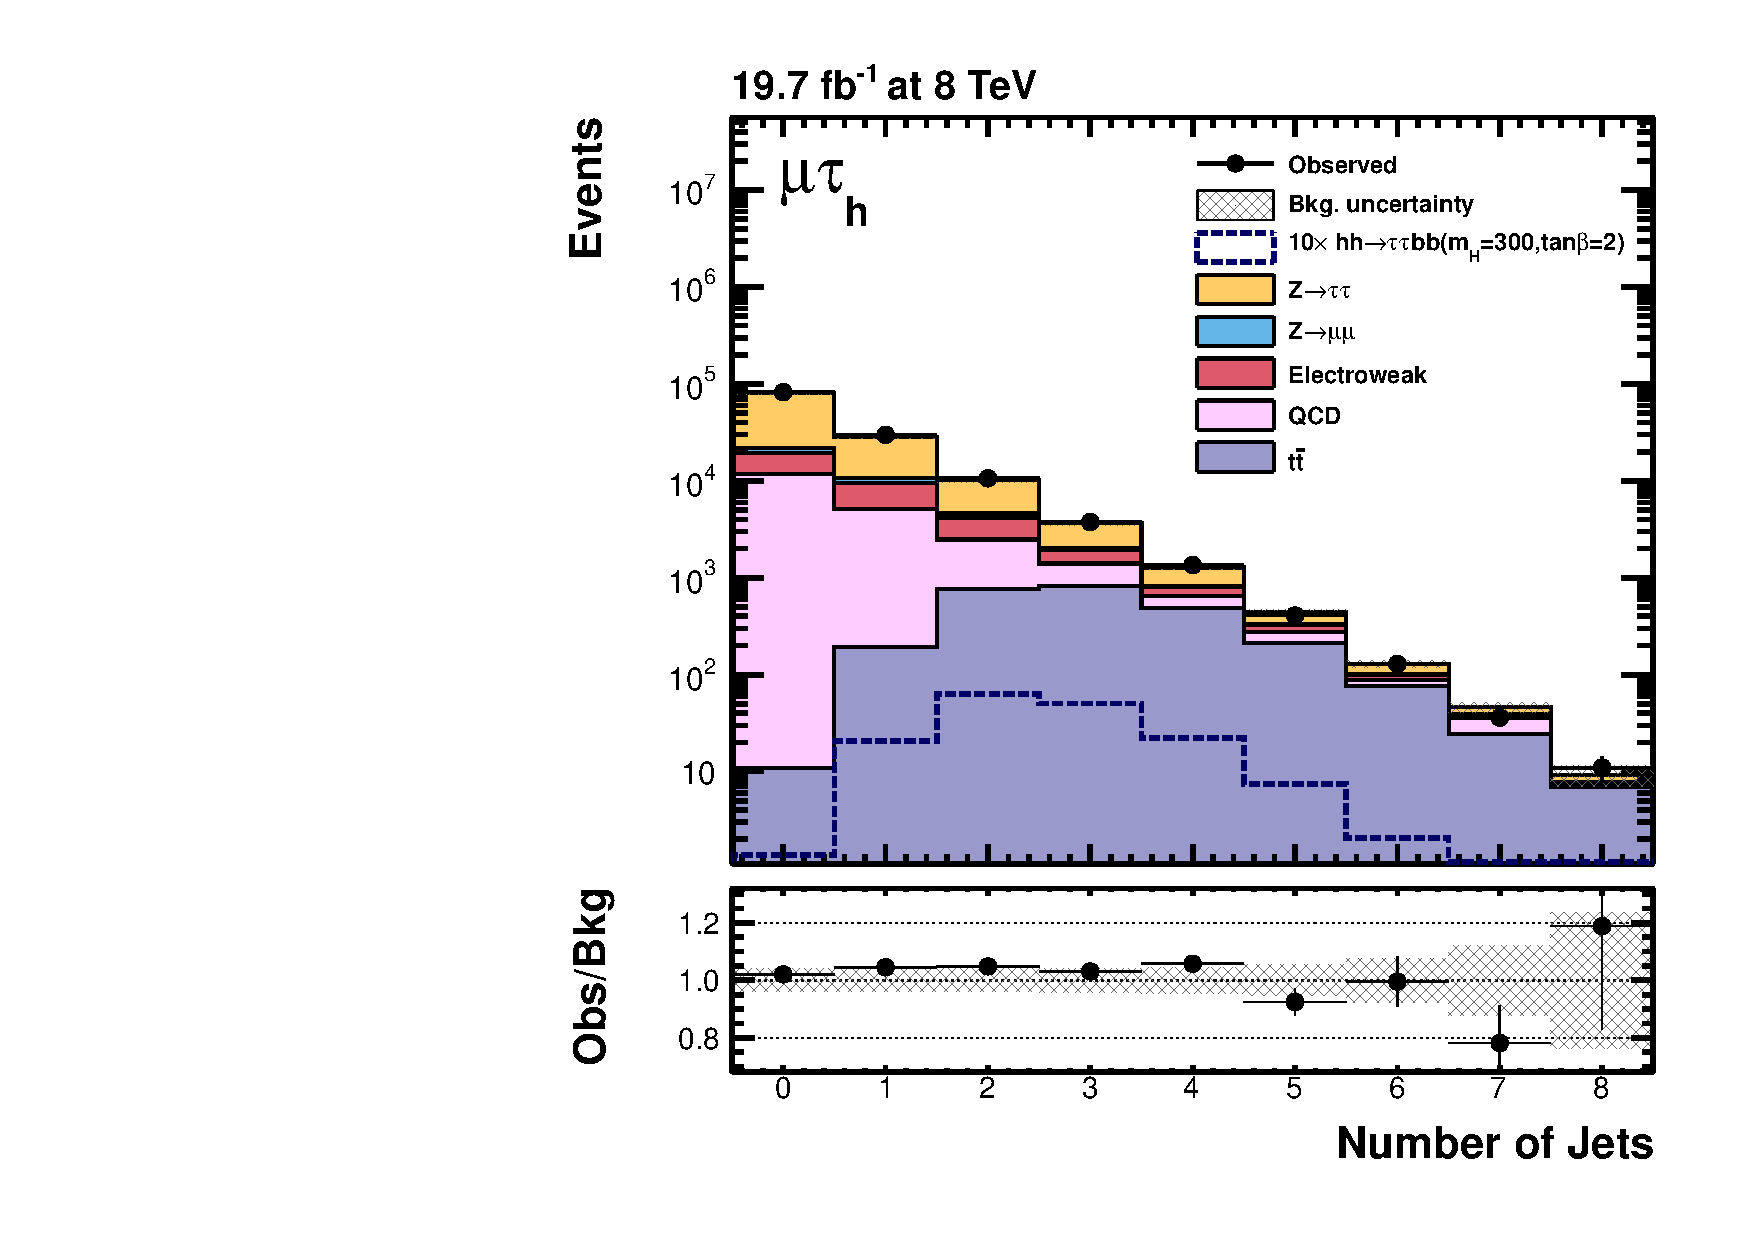
\includegraphics[width=0.5\textwidth]
      {plots/Hhh/n_prebjets_inclusive_mt_2012_log.pdf}}
\subfloat[]{
    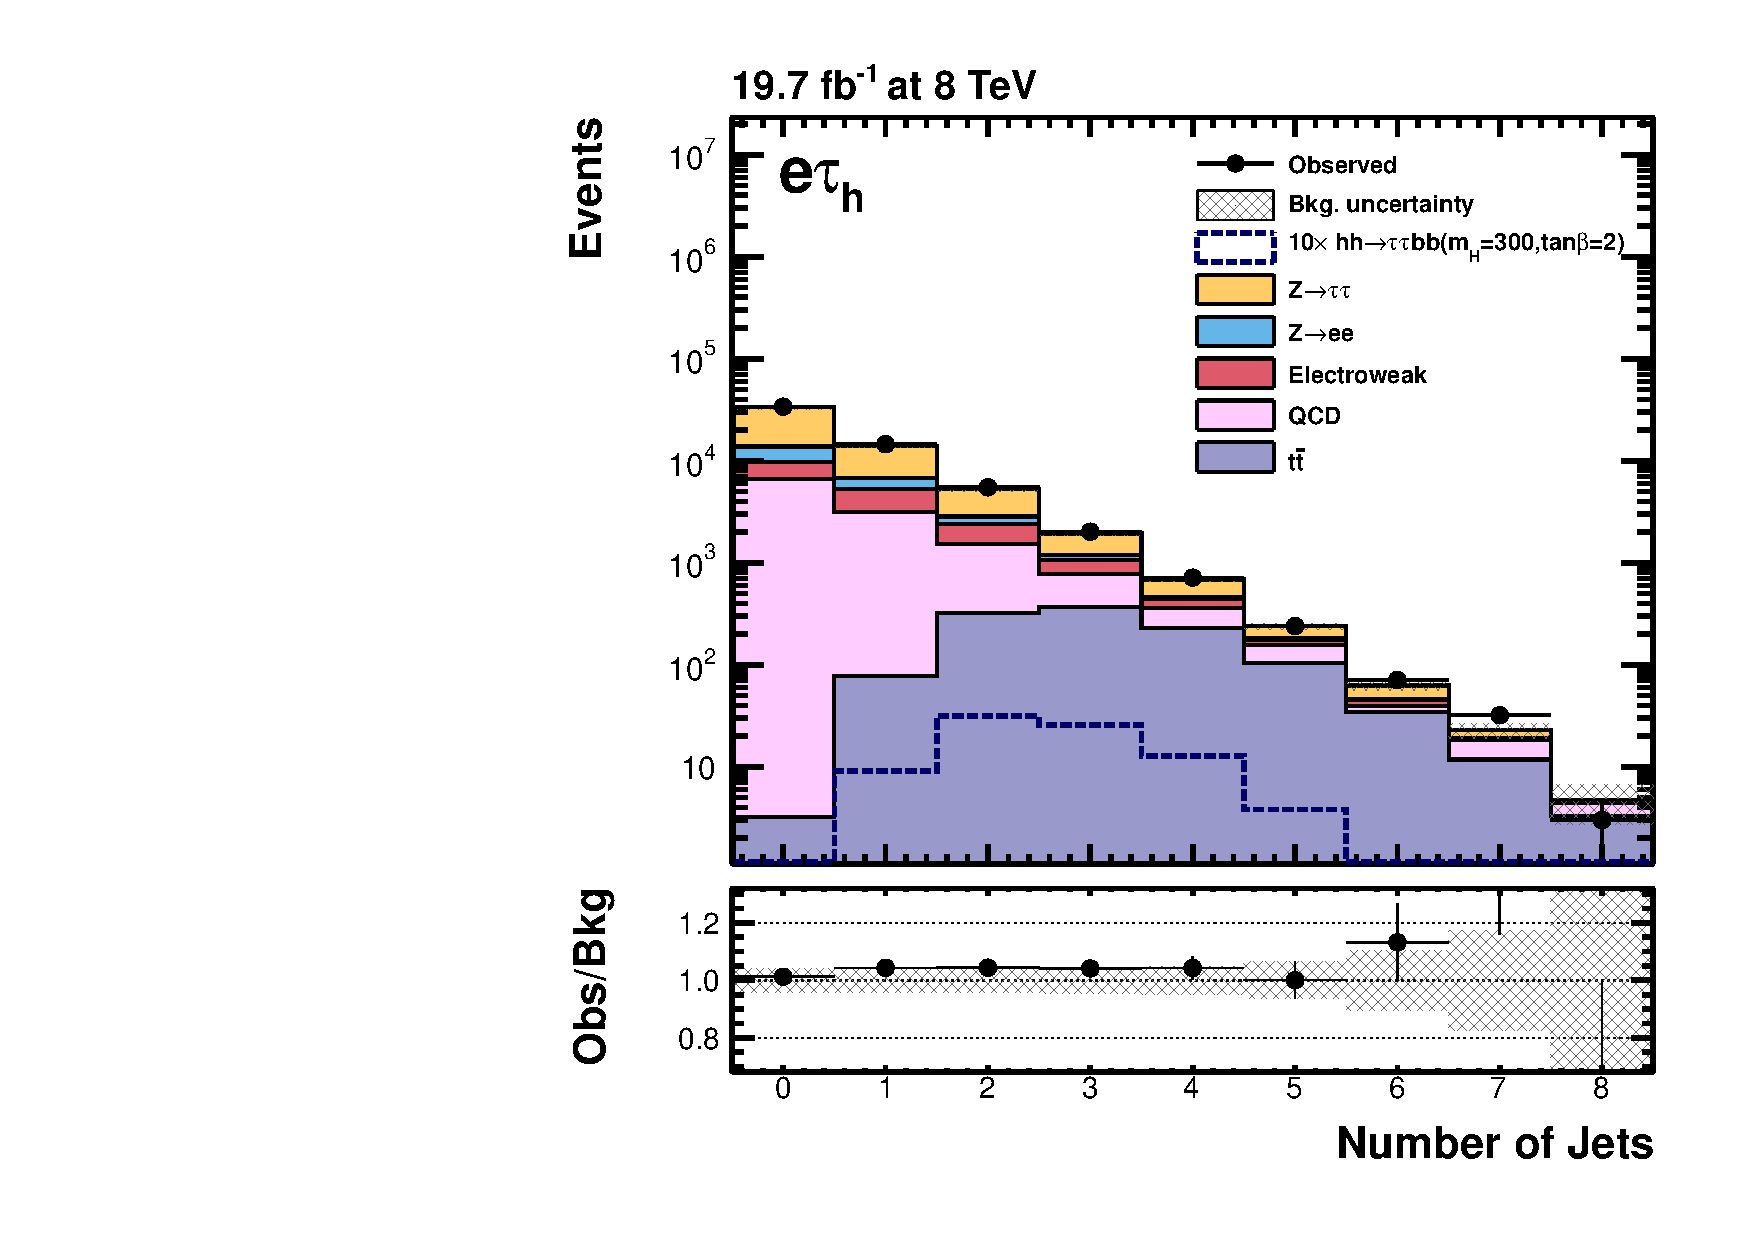
\includegraphics[width=0.5\textwidth] 
      {plots/Hhh/n_prebjets_inclusive_et_2012_log.pdf}} 

\end{center}
\caption[Number of jets in inclusive $\Pgt\Pgt$ events in backgrounds and
$\PH\to\Ph\Ph$ signal.]{
Number of jets in inclusive $\Pgt\Pgt$ events in backgrounds and
$\PH\to\Ph\Ph$ signal. Distribution shown for events in the $\mutau$ (a) and $\etau$
(b) channels.}
\label{fig:Hhhnjets}
\end{figure} 

\begin{figure}
\begin{center}
\subfloat[]{
    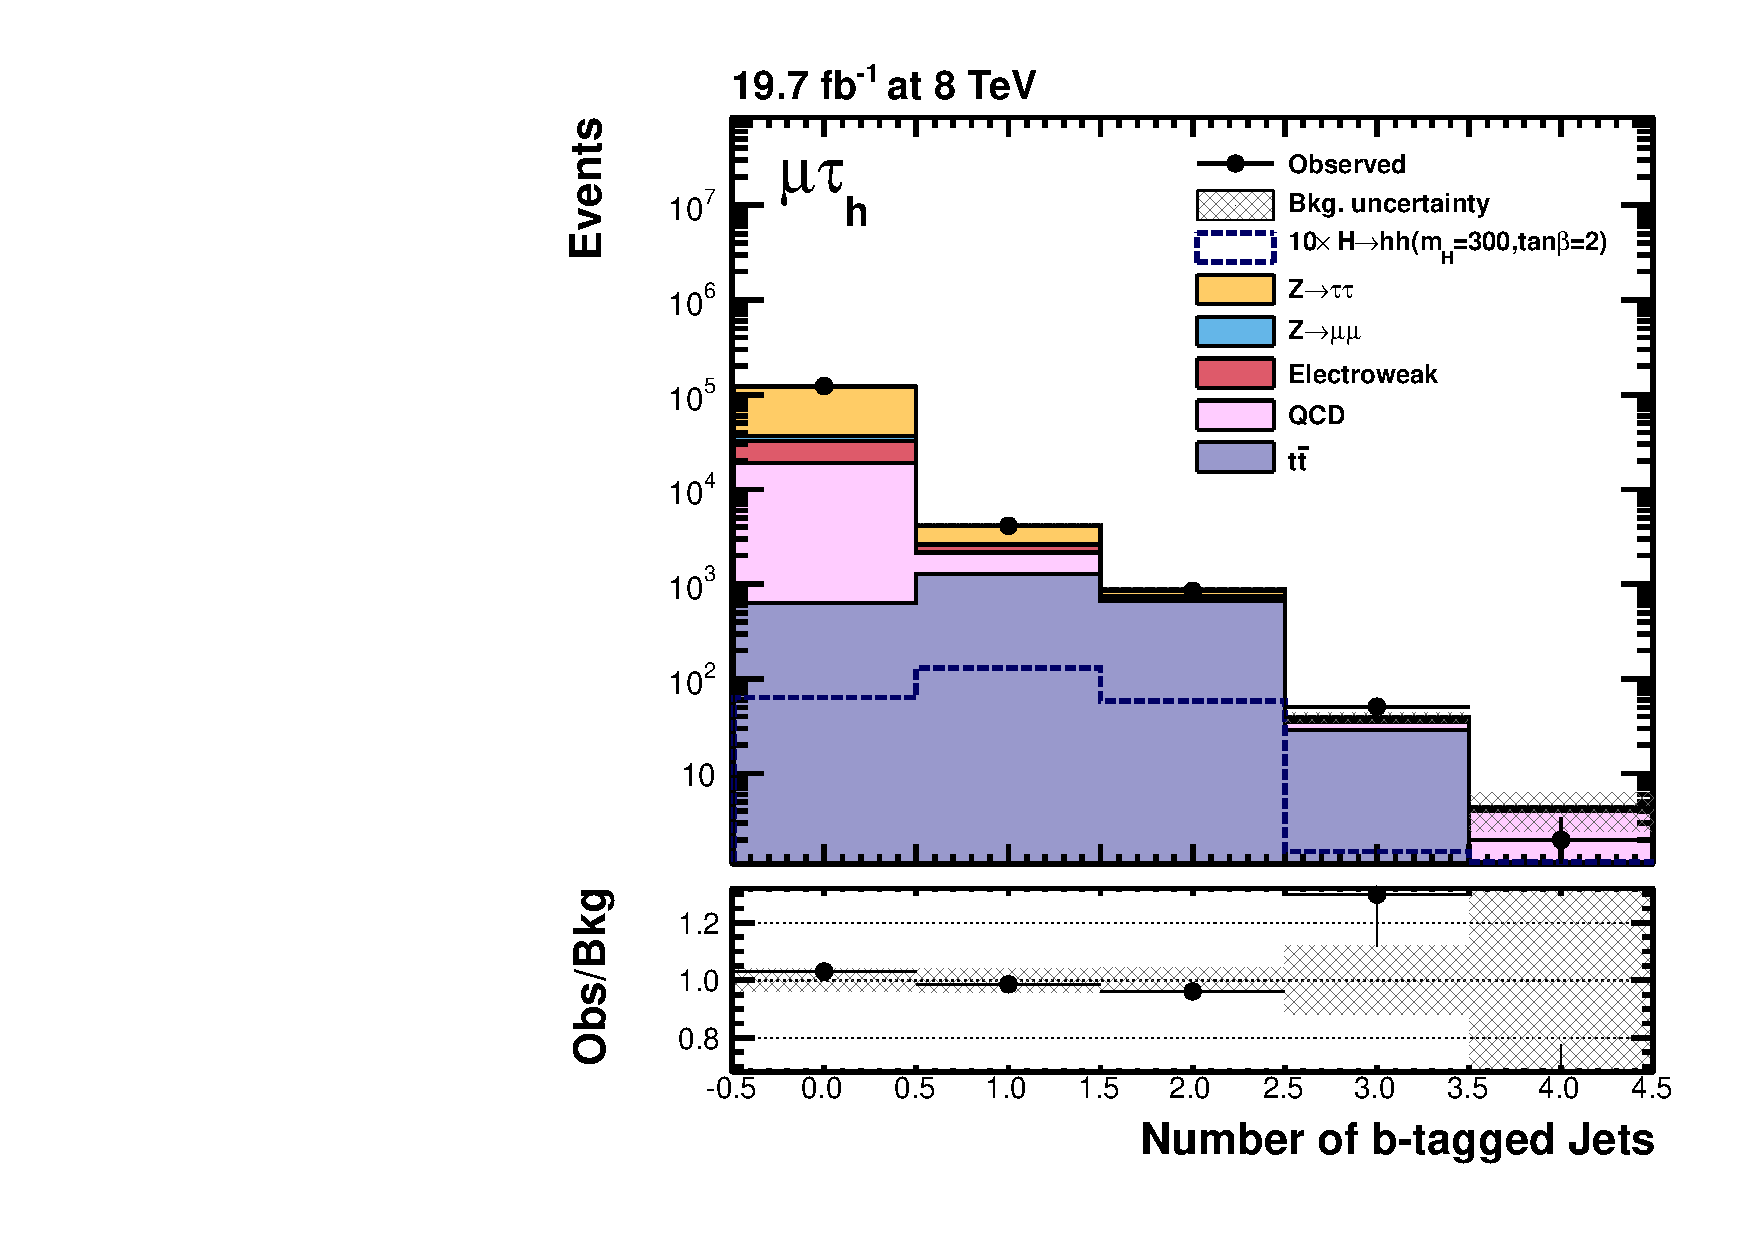
\includegraphics[width=0.5\textwidth]
      {plots/Hhh/n_prebjets_SF_inclusive_mt_2012_log.pdf}}
\subfloat[]{
    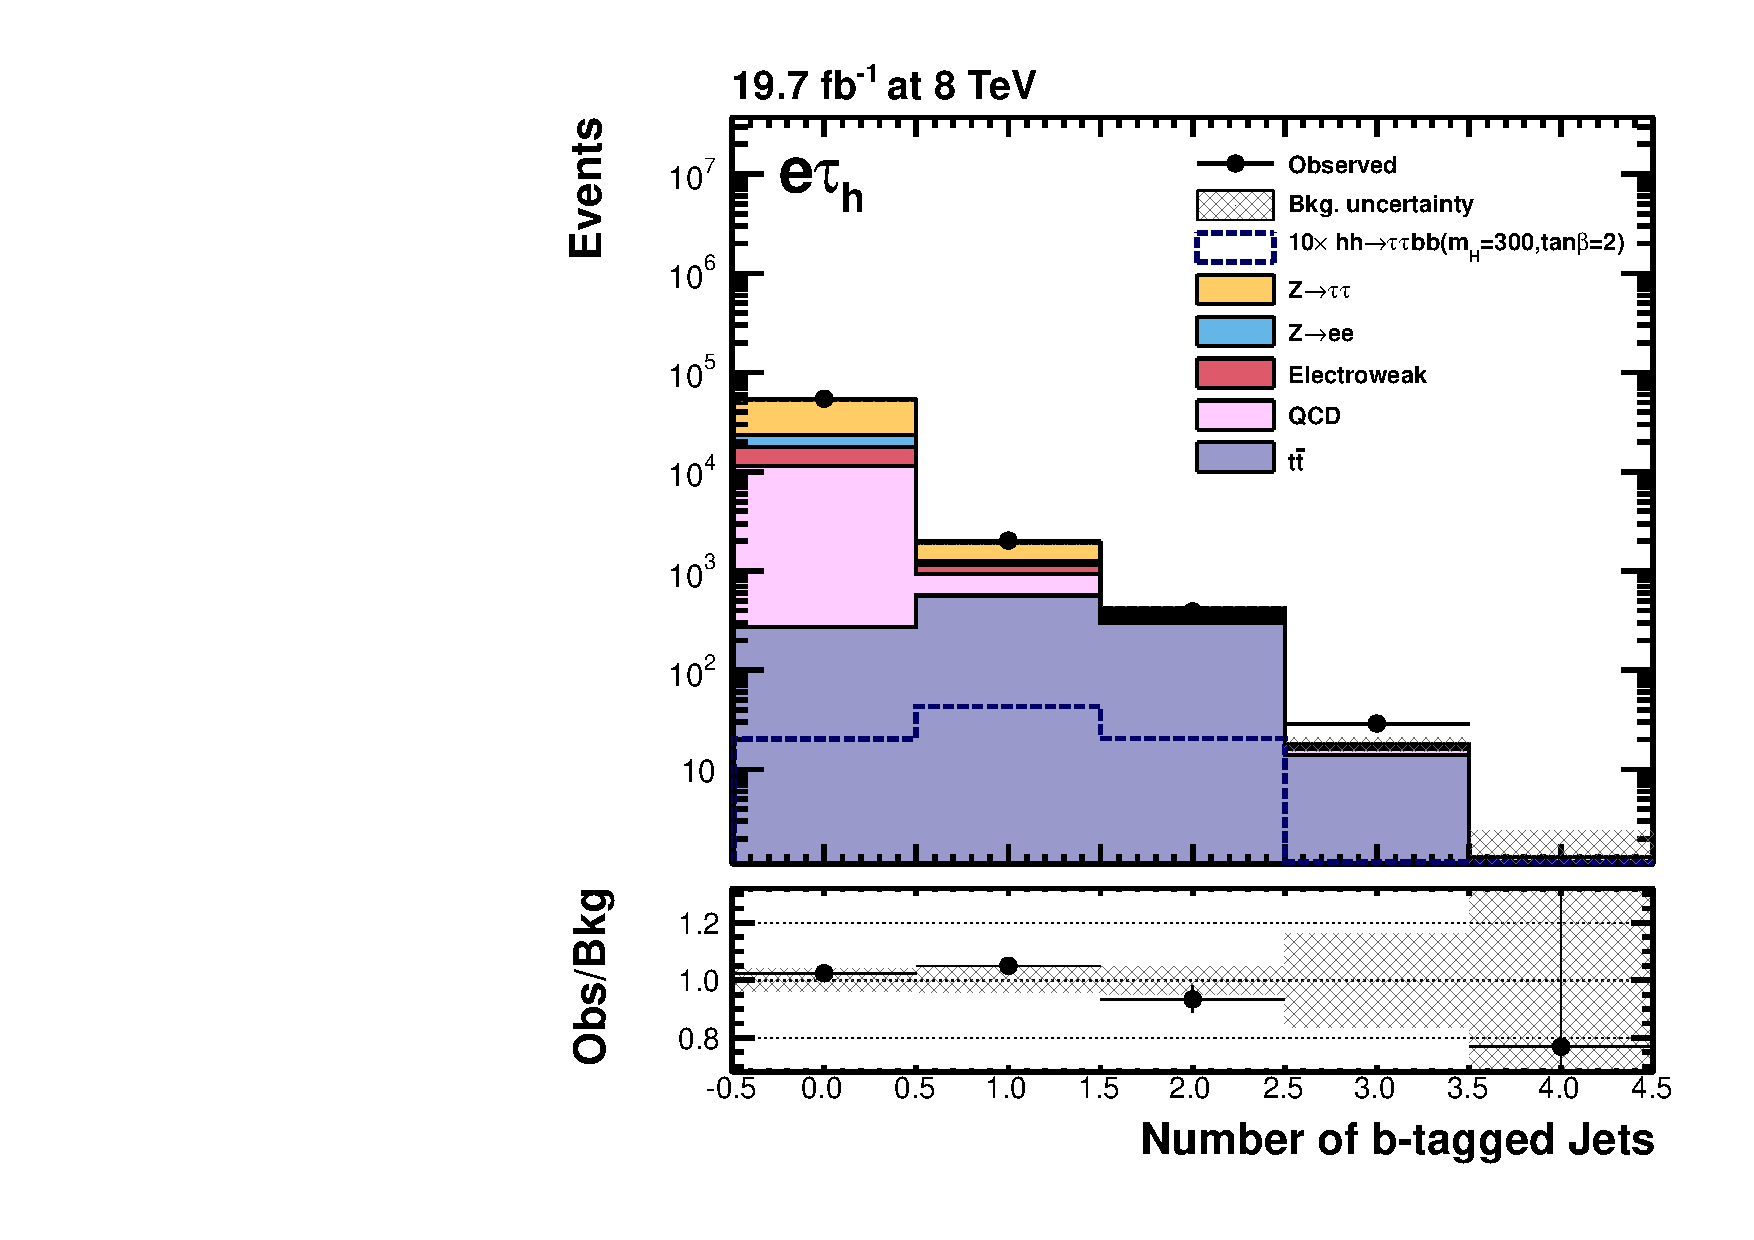
\includegraphics[width=0.5\textwidth] 
      {plots/Hhh/n_prebjets_SF_inclusive_et_2012_log.pdf}} 

\end{center}
\caption[Number of b-tagged jets in inclusive $\Pgt\Pgt$ events in backgrounds and
$\PH\to\Ph\Ph$ signal.]{
Number of b-tagged jets in inclusive $\Pgt\Pgt$ events in backgrounds and
$\PH\to\Ph\Ph$ signal. Distribution shown for events in the $\mutau$ (a) and $\etau$
(b) channels. }
\label{fig:Hhhnbjets}
\end{figure} 


\begin{figure}
\begin{center}
\subfloat[]{
    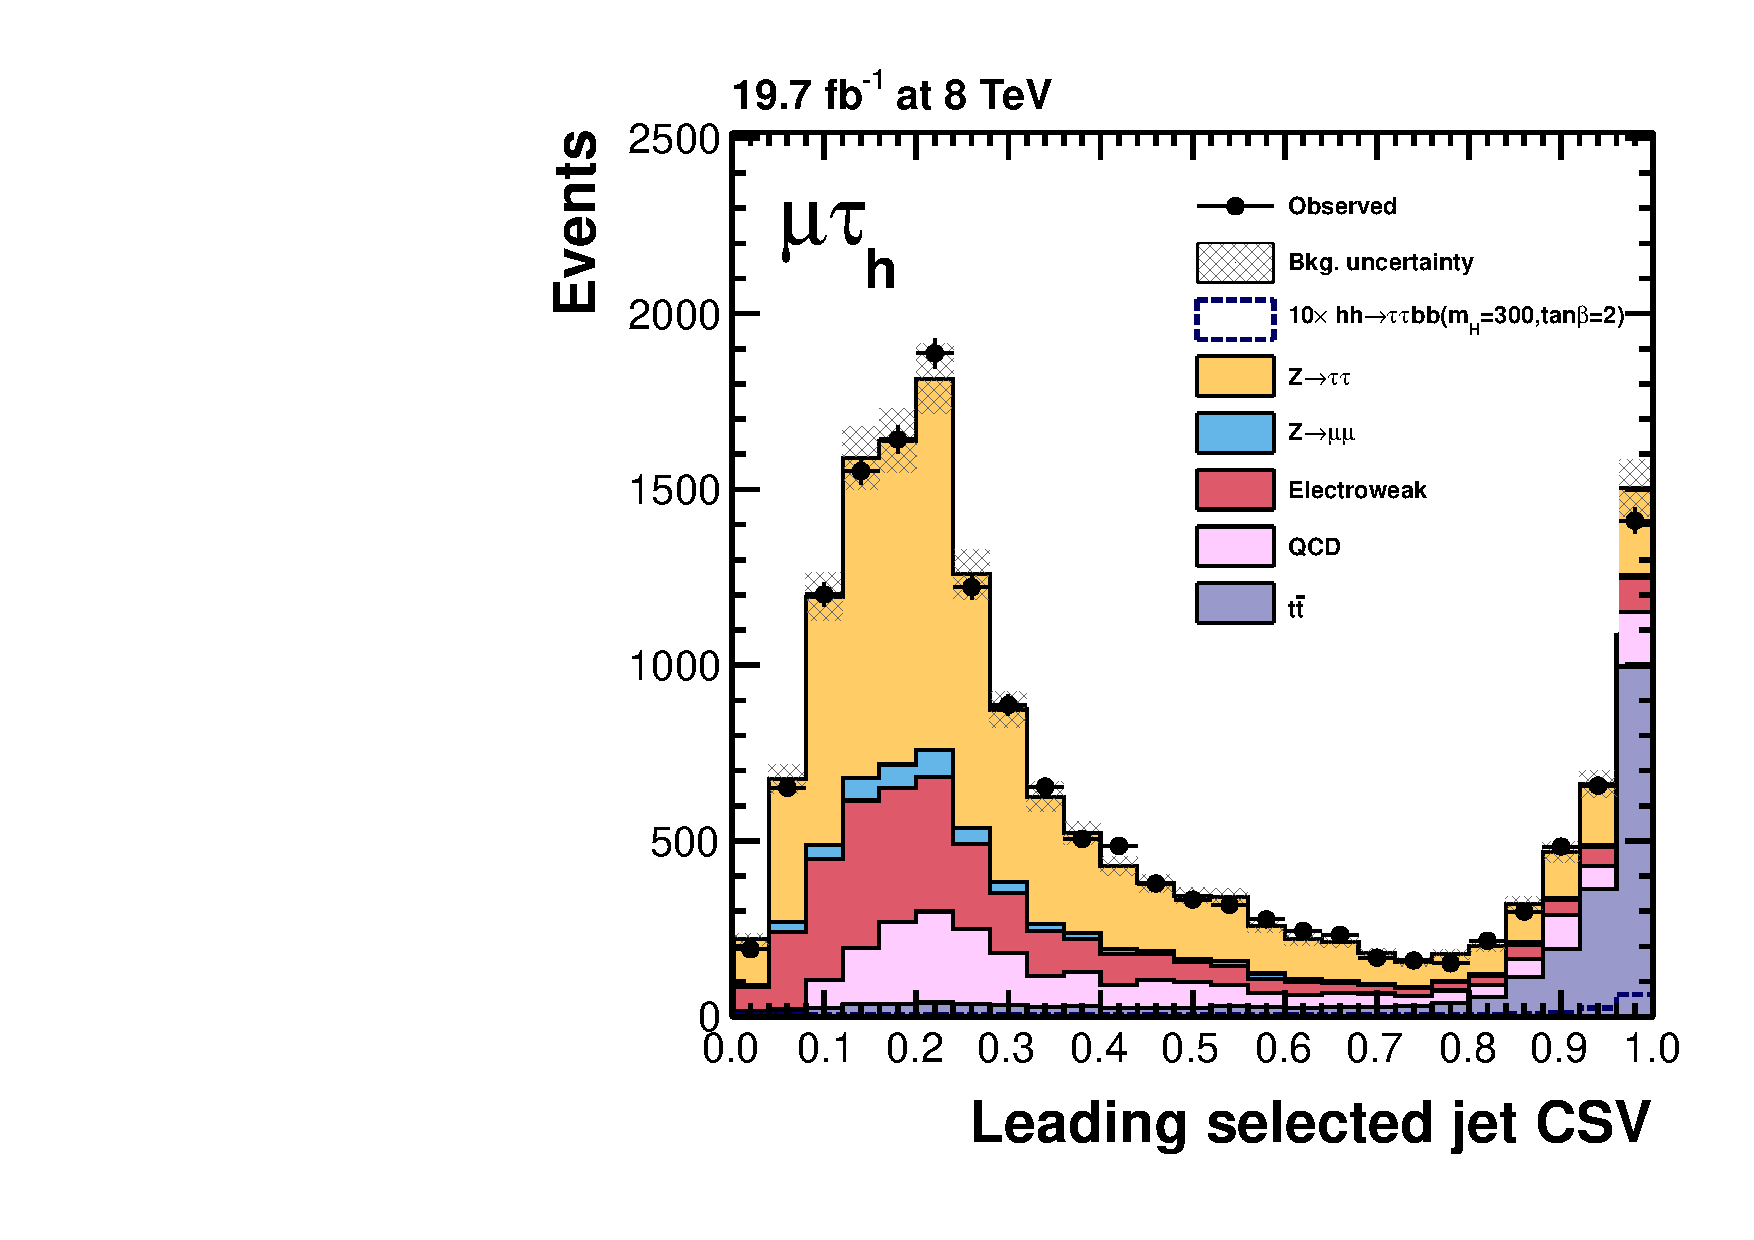
\includegraphics[width=0.5\textwidth]
      {plots/Hhh/prebjetbcsv_1_2jetinclusive_mt_2012.pdf}}
\subfloat[]{
    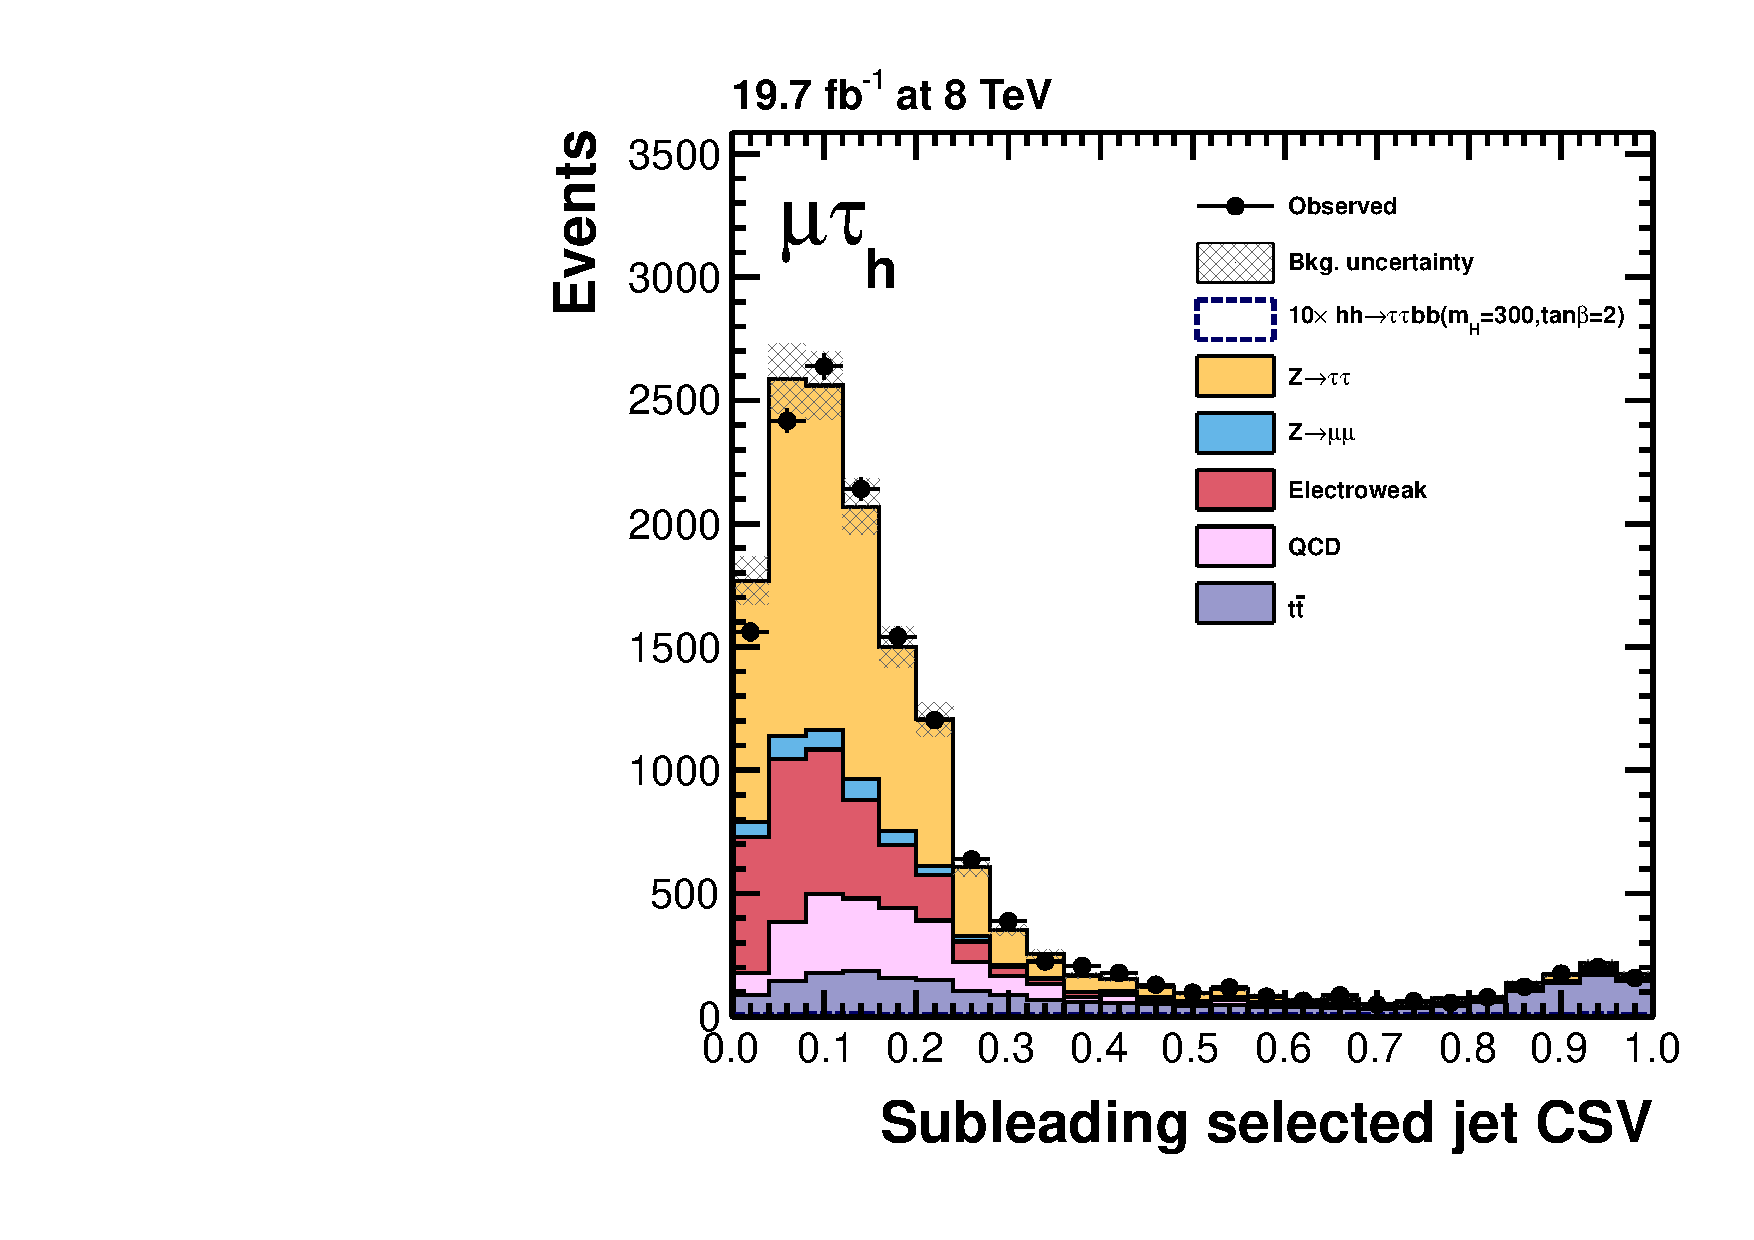
\includegraphics[width=0.5\textwidth] 
      {plots/Hhh/prebjetbcsv_2_2jetinclusive_mt_2012.pdf}} 

\end{center}
\caption{
Values of the \ac{CSV} b-tagging discriminator for the highest \ac{CSV}
(leading) jet in the event (left) and second highest (subleading) \ac{CSV} jet
in the event (right), for events with at least two jets in the $\mutau$ channel.}
\label{fig:Hhhcsv}
\end{figure} 

Finally, events are categorised depending on whether zero, one or two of the selected jets pass the
medium \ac{CSV} b-tagging working point. This allows all of the potential signal
events in the inclusive selection which have at least two jets to be retained,
whilst separating them into regions with very different background compositions
and varying signal sensitivity. The categories are defined as follows:

\begin{itemize}
\item \textbf{2jet--0tag} 
Events in this category are such that neither of the leading and subleading jets
passes the medium \ac{CSV} working point. This category only collects a small amount
of signal and is dominated by backgrounds, in particular $\ZToTauTau$, QCD and
$\WJets$.
\item \textbf{2jet--1tag} 
Events in this category are such that only the leading but not the subleading jet
passes the medium \ac{CSV} working point. This category collects more than half of
the signal events, but is still quite high in backgrounds, including increased
$\ttbar$.
\item \textbf{2jet--2tag} 
Events in this category are such that both the leading and subleading jets
pass the medium \ac{CSV} working point. This is the most signal-sensitive category,
since the requirement of 2 b-tagged jets greatly reduces the backgrounds with
the exception of $\ttbar$.  
\end{itemize}

In signal events of all heavy Higgs boson mass hypotheses, both the reconstructed $m_{\Pqb\Pqb}$ and
$m_{\Pgt\Pgt}$ will be consistent with a $125\,\GeV$ $\Ph$ decay.
Figures \ref{fig:2jet0tagmttmbb}, \ref{fig:2jet1tagmttmbb} and
\ref{fig:2jet2tagmttmbb} illustrate the distributions of $m_{\Pgt\Pgt}$ and
$m_{\Pqb\Pqb}$ for events in the 2jet--0tag, 2jet--1tag and 2jet--2tag
categories respectively. These distributions
illustrate the different background compositions and varying sensitivities of
the categories. It can also be seen from the 2jet--1tag and 2jet--2tag categories 
that the signal peaks around $125\,\GeV$ in
both variables, whereas the backgrounds are more spread across the mass range. 
This fact is exploited to greatly
enhance the selection of signal over background events, by applying cuts in
windows of $70 < m_{\Pqb\Pqb} < 150\,\GeV$ and $90 < m_{\Pgt\Pgt} < 150\,\GeV$ to
select signal-like events. For all subsequent results in this chapter these cuts
on $m_{\Pqb\Pqb}$ and $m_{\Pgt\Pgt}$ are applied as part of the baseline event
selection unless otherwise stated. 

\begin{figure}
\begin{center}
\subfloat[]{
    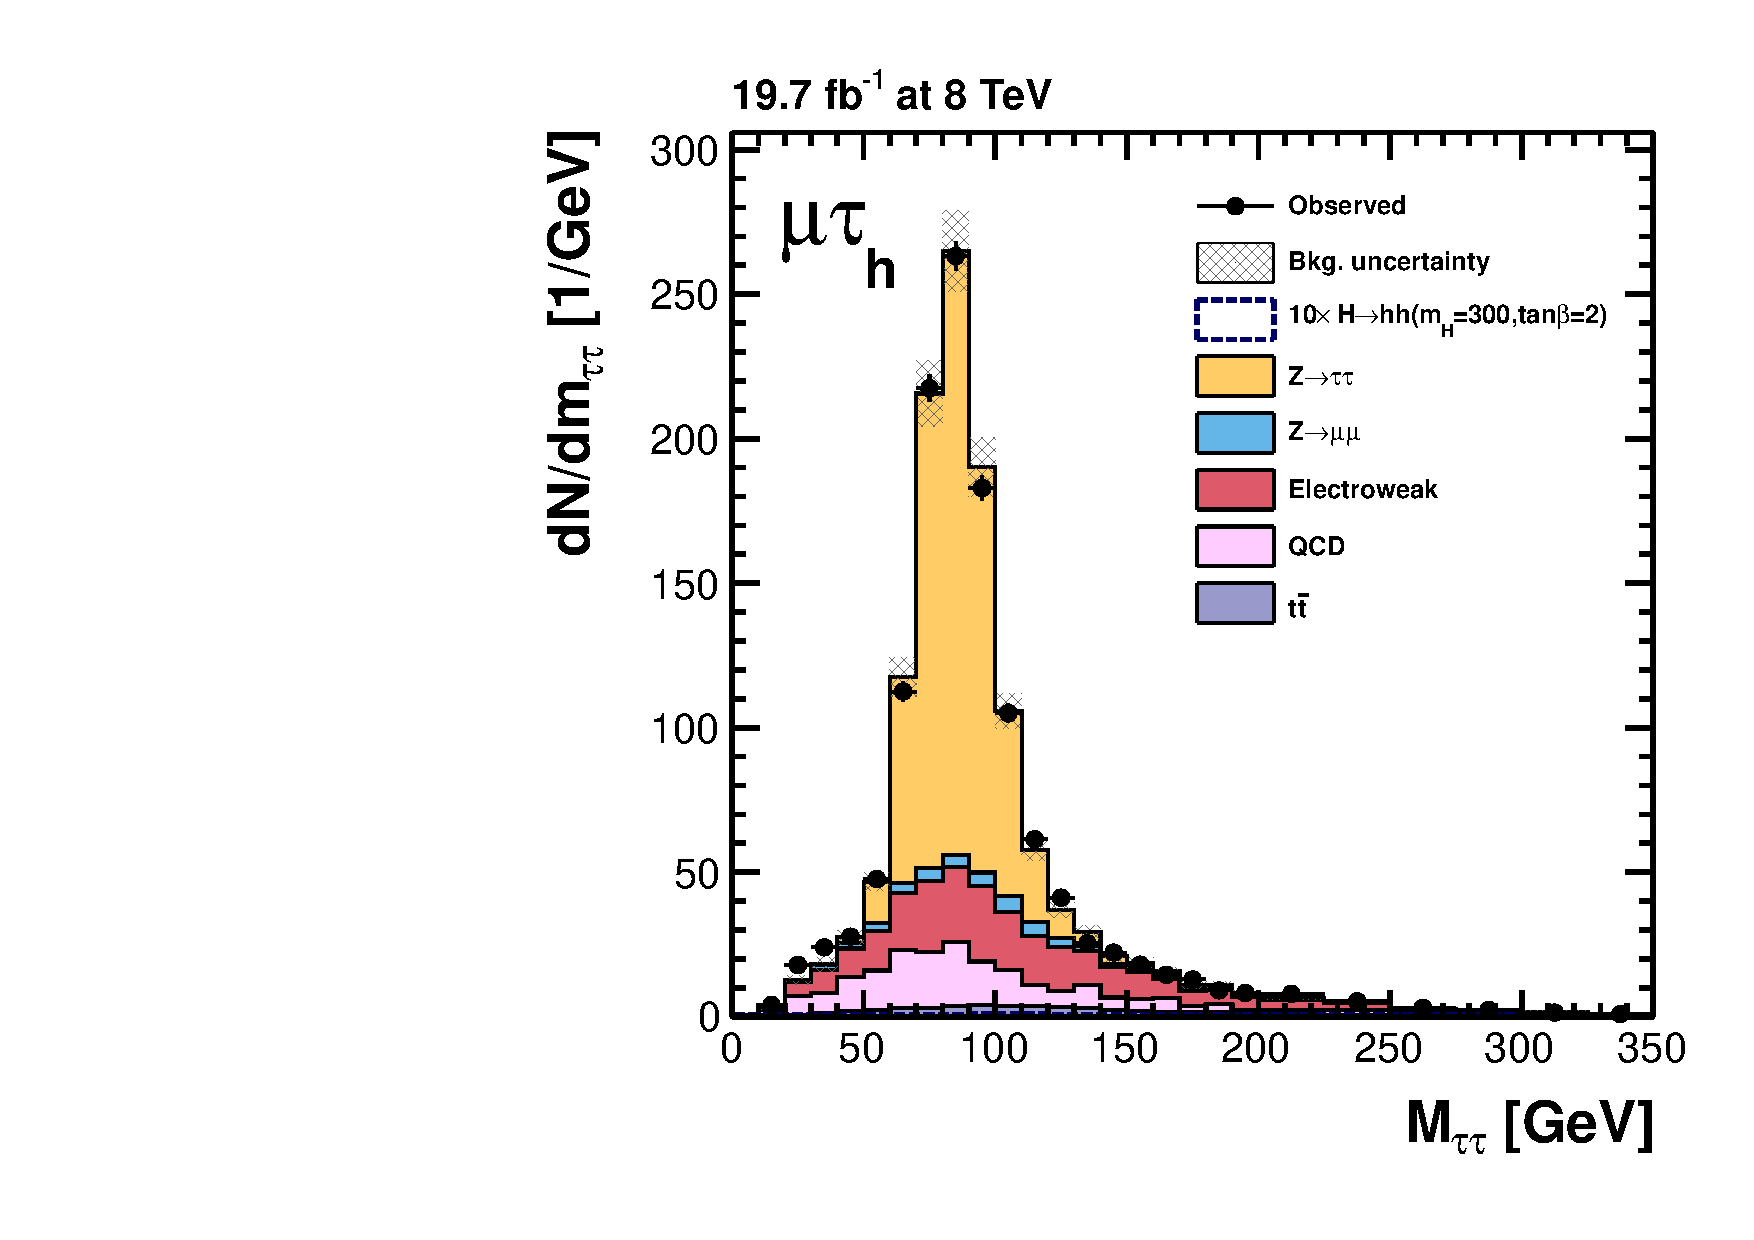
\includegraphics[width=0.5\textwidth]
      {plots/Hhh/m_sv_2jet0tagSF_mt_2012.pdf}}
\subfloat[]{
    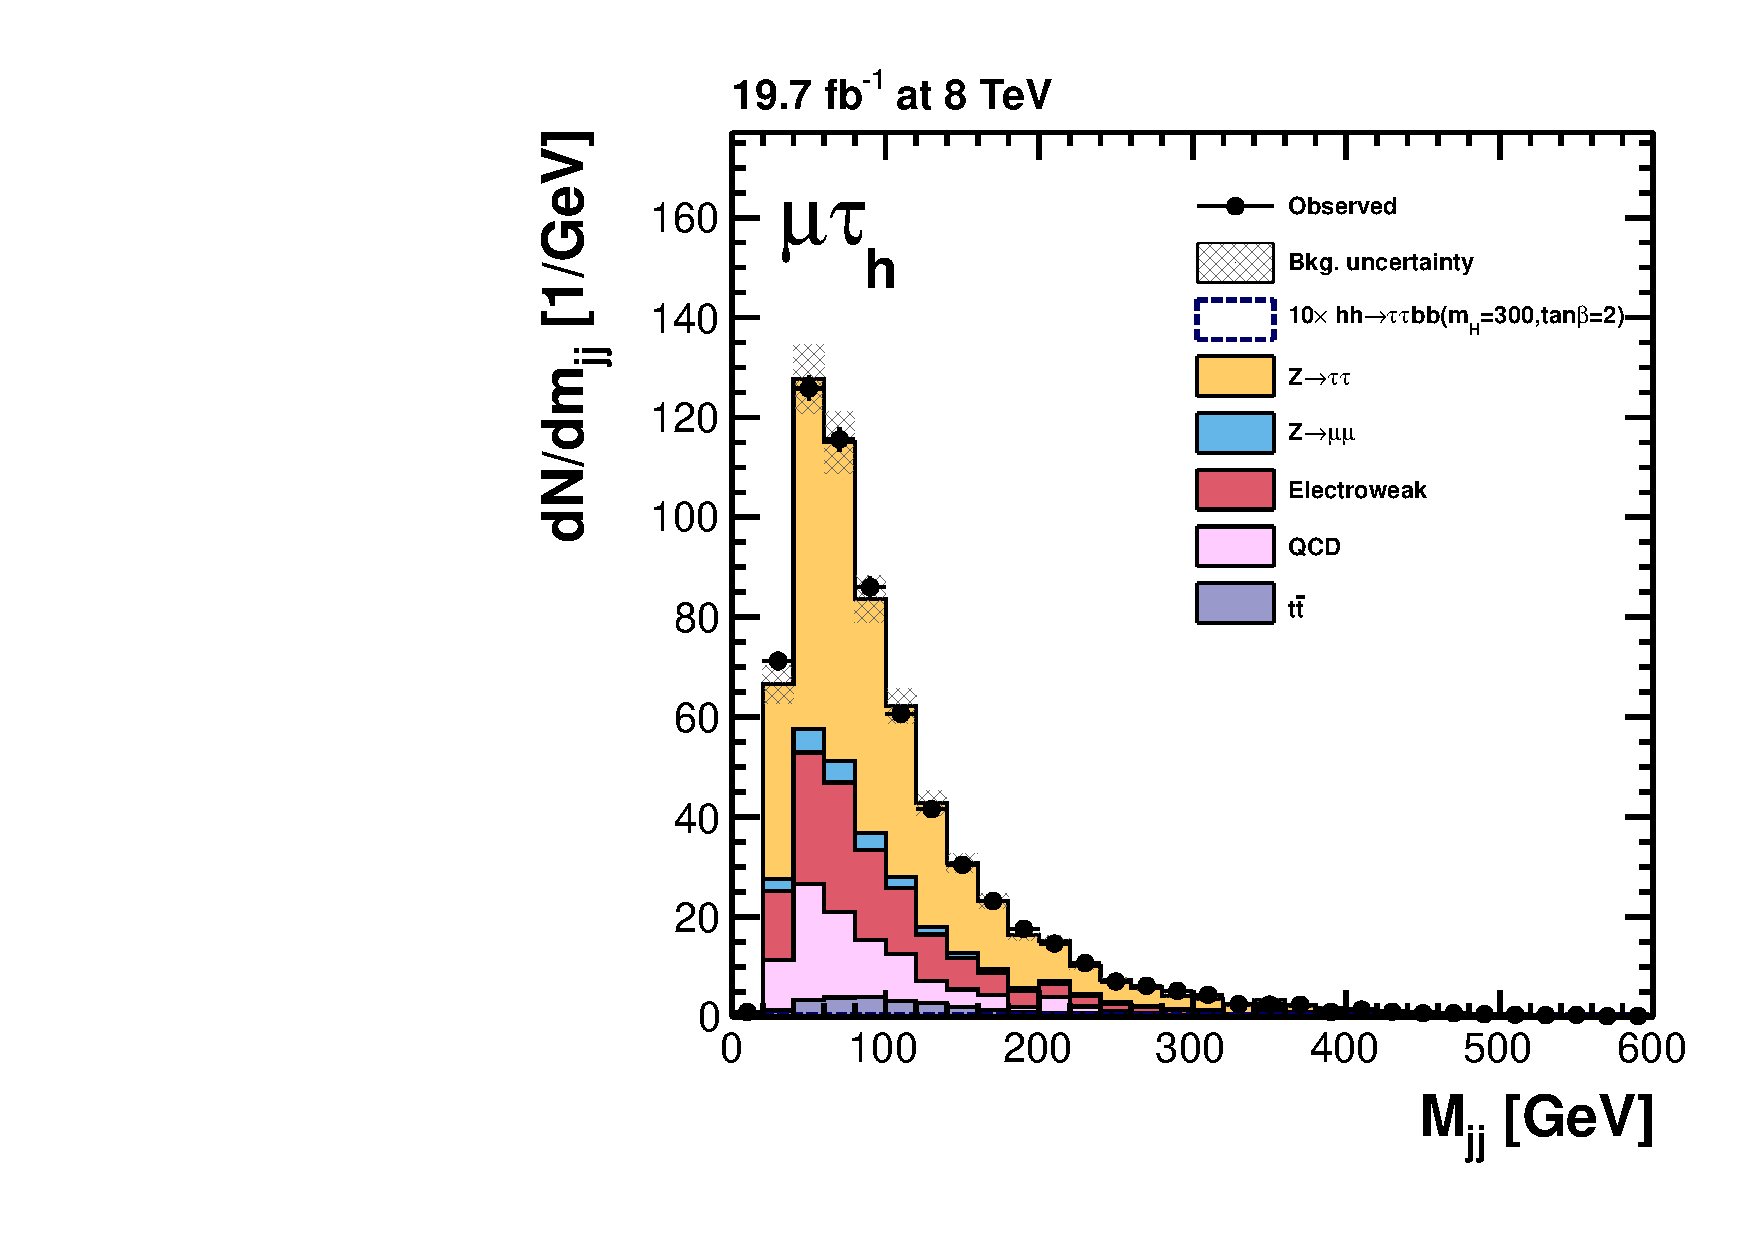
\includegraphics[width=0.5\textwidth] 
      {plots/Hhh/prebjet_mjj_2jet0tagSF_mt_2012.pdf}} 

\subfloat[]{
    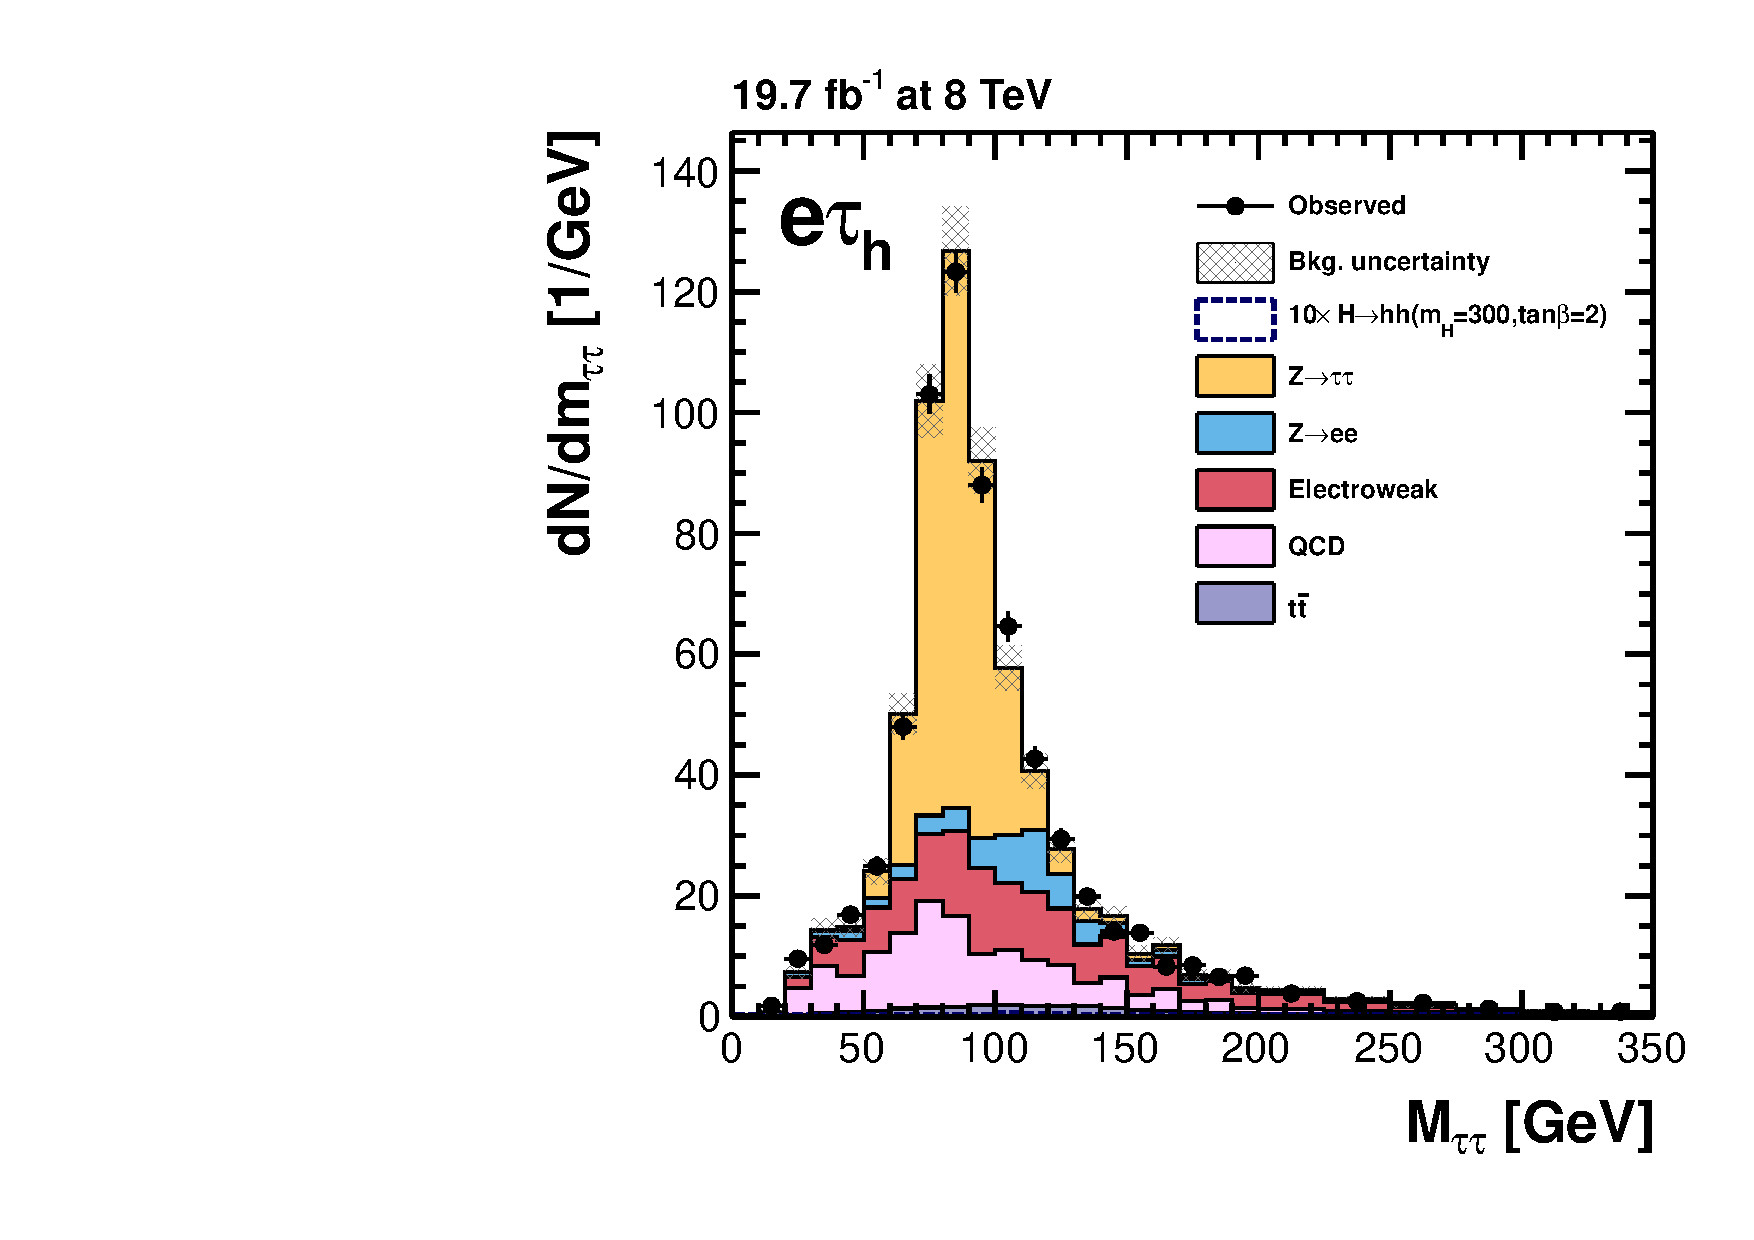
\includegraphics[width=0.5\textwidth]
      {plots/Hhh/m_sv_2jet0tagSF_et_2012.pdf}}
\subfloat[]{
    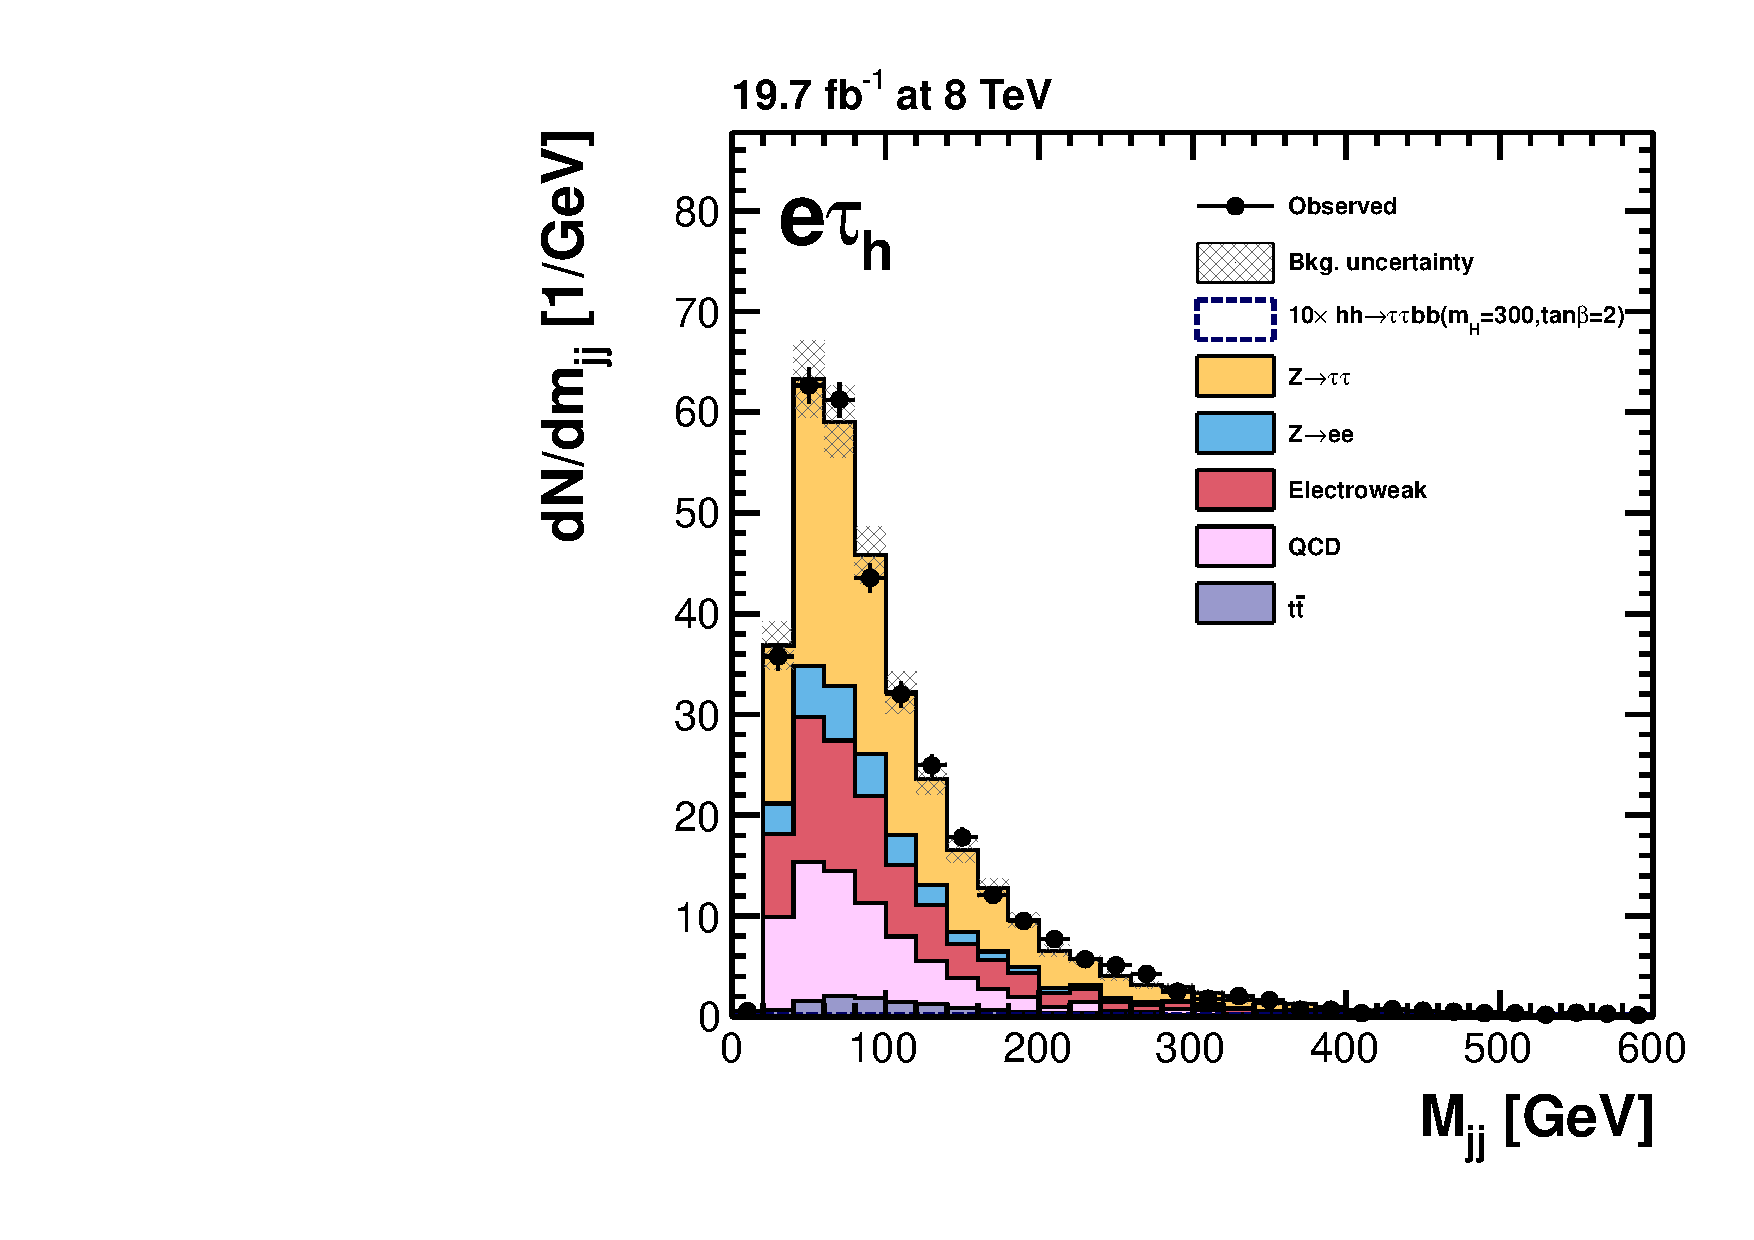
\includegraphics[width=0.5\textwidth] 
      {plots/Hhh/prebjet_mjj_2jet0tagSF_et_2012.pdf}} 
\end{center}
\caption[Distributions of $m_{\Pgt\Pgt}$ (left) and $m_{\Pqb\Pqb}$ (right) in the $\mutau$ (top) and
$\etau$ (bottom) channels for the 2jet--0tag category.]{
Distributions of $m_{\Pgt\Pgt}$ (left) and $m_{\Pqb\Pqb}$ (right) in the $\mutau$ (top) and
$\etau$ (bottom) channels for the 2jet--0tag category. The signal cannot be seen
in these figures since this category is background dominated.}
\label{fig:2jet0tagmttmbb}
\end{figure} 

\begin{figure}
\begin{center}
\subfloat[]{
    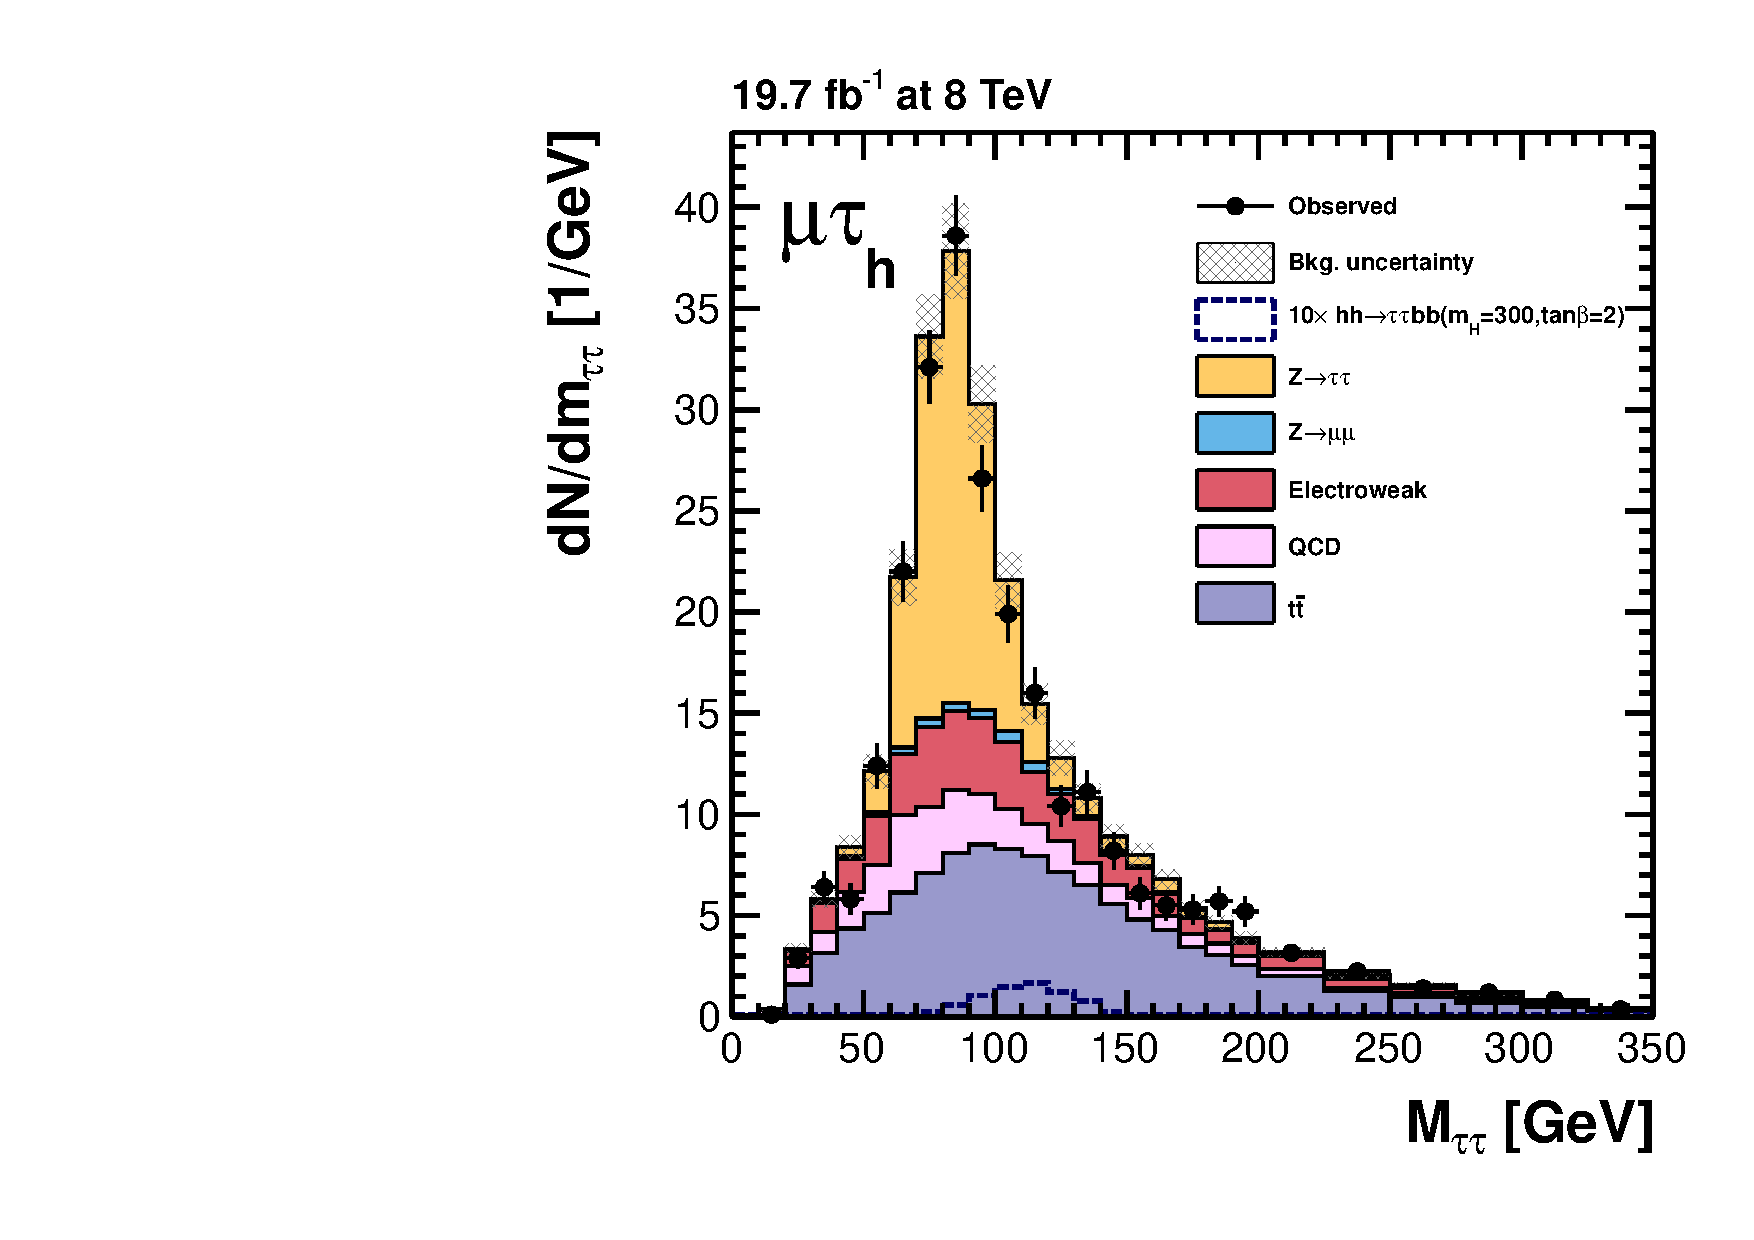
\includegraphics[width=0.5\textwidth]
      {plots/Hhh/m_sv_2jet1tagSF_mt_2012.pdf}}
\subfloat[]{
    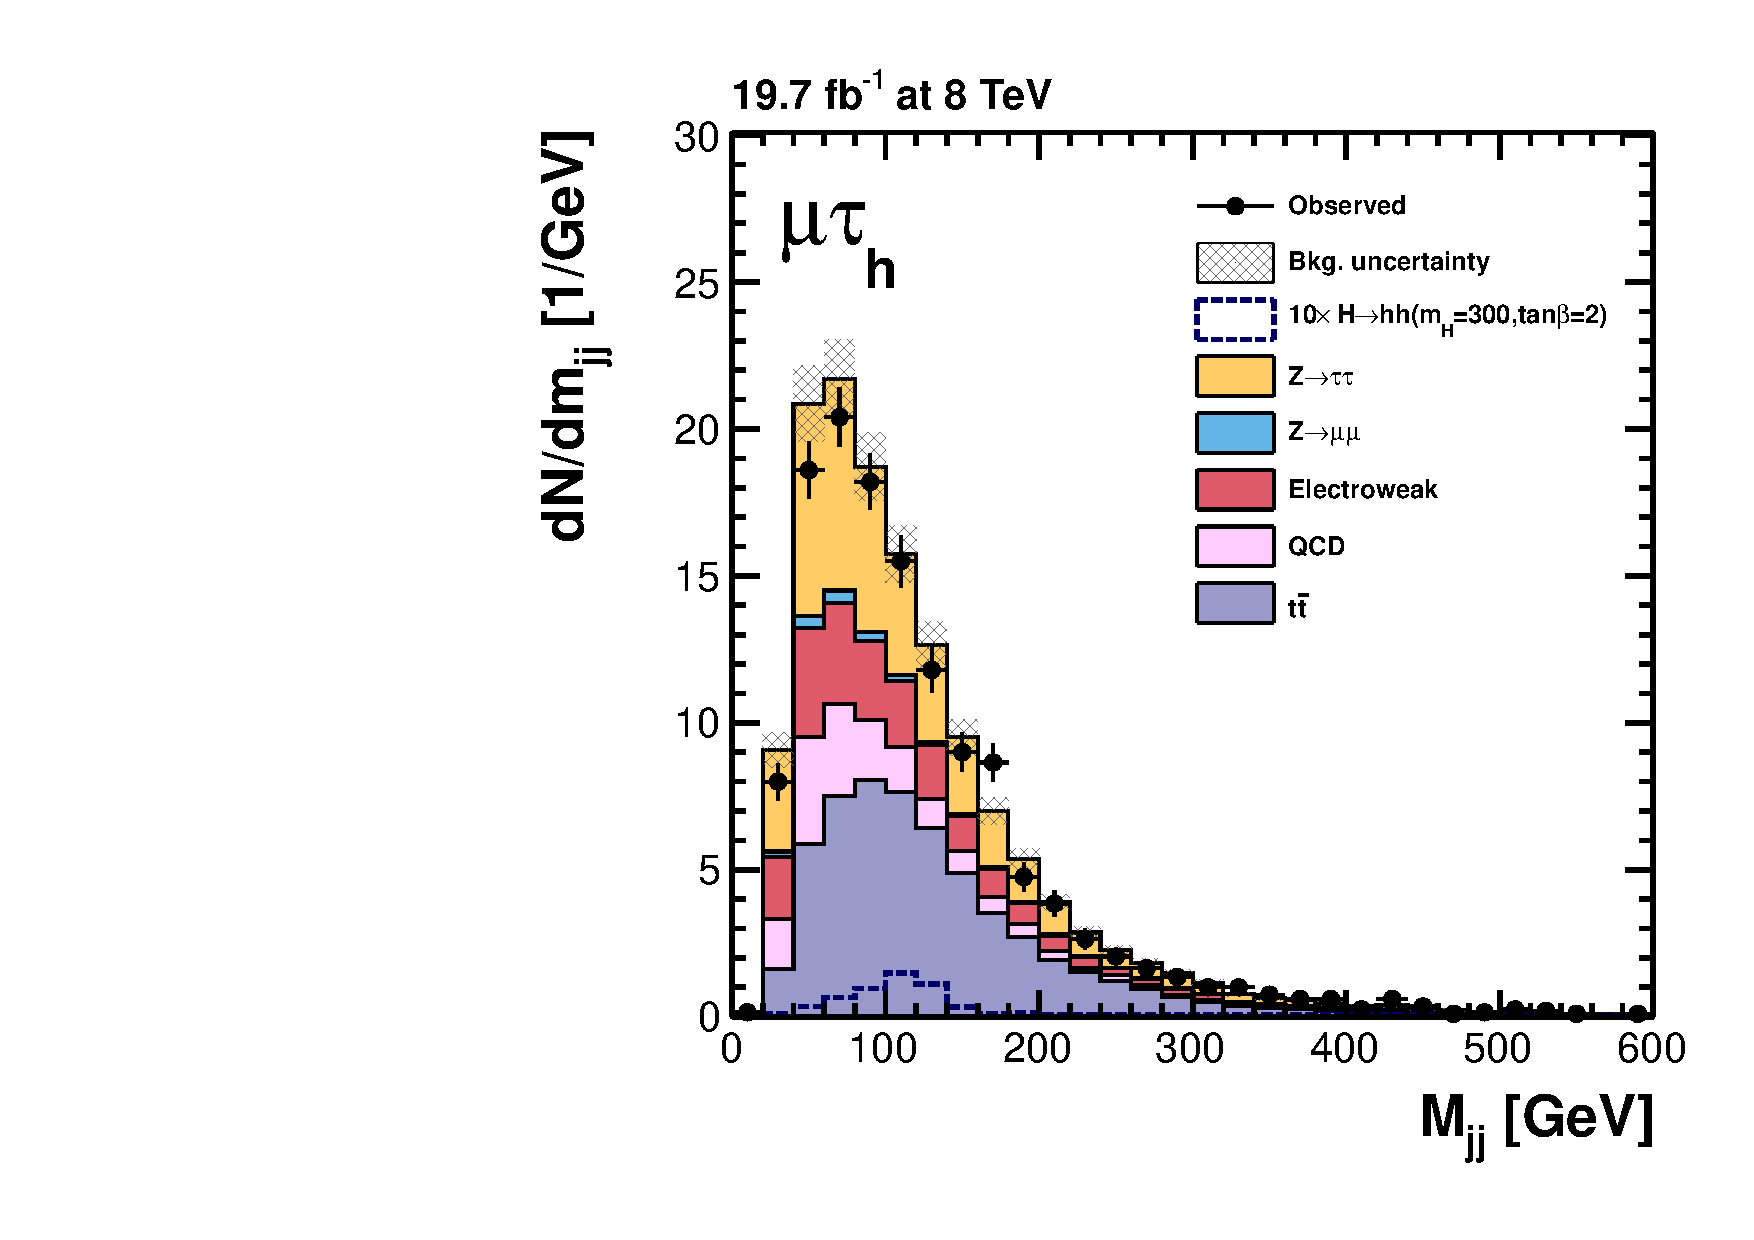
\includegraphics[width=0.5\textwidth] 
      {plots/Hhh/prebjet_mjj_2jet1tagSF_mt_2012.pdf}} 

\subfloat[]{
    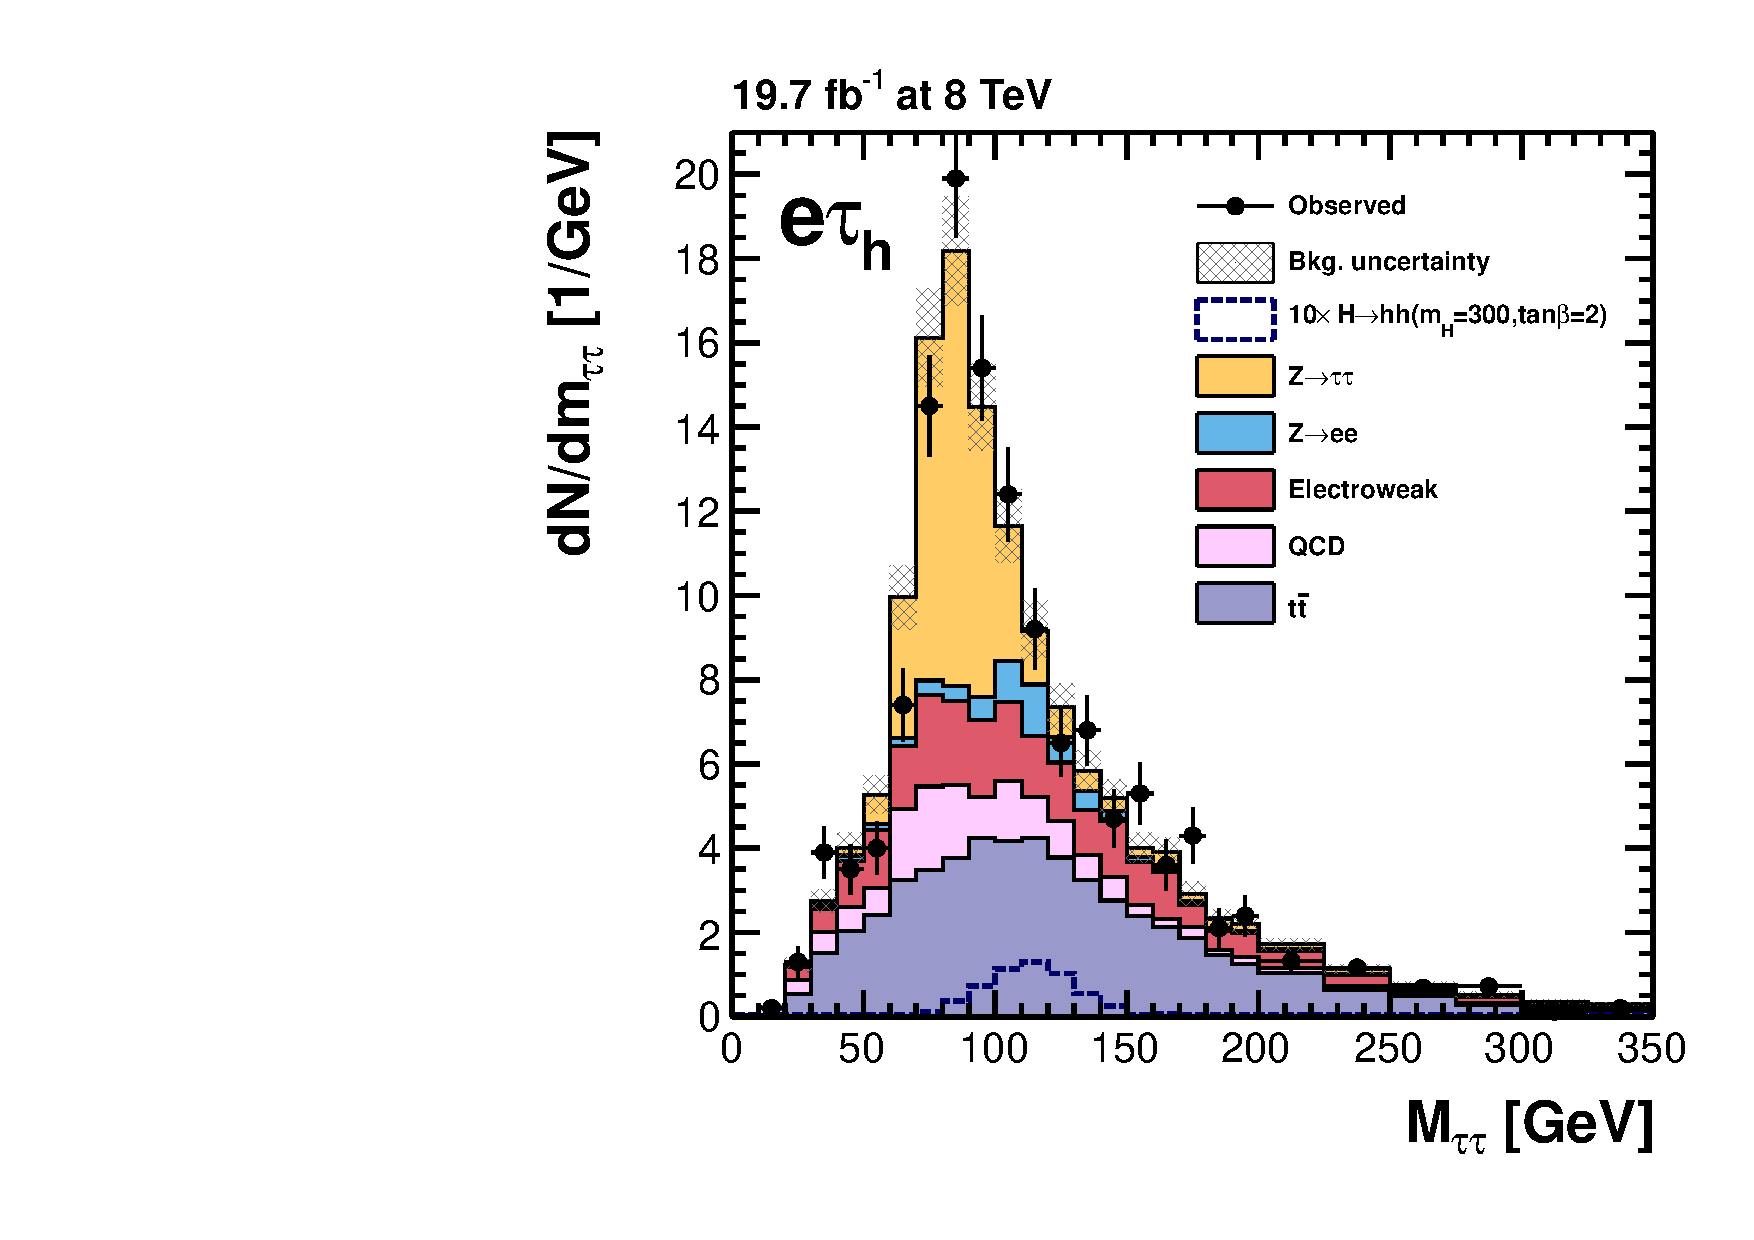
\includegraphics[width=0.5\textwidth]
      {plots/Hhh/m_sv_2jet1tagSF_et_2012.pdf}}
\subfloat[]{
    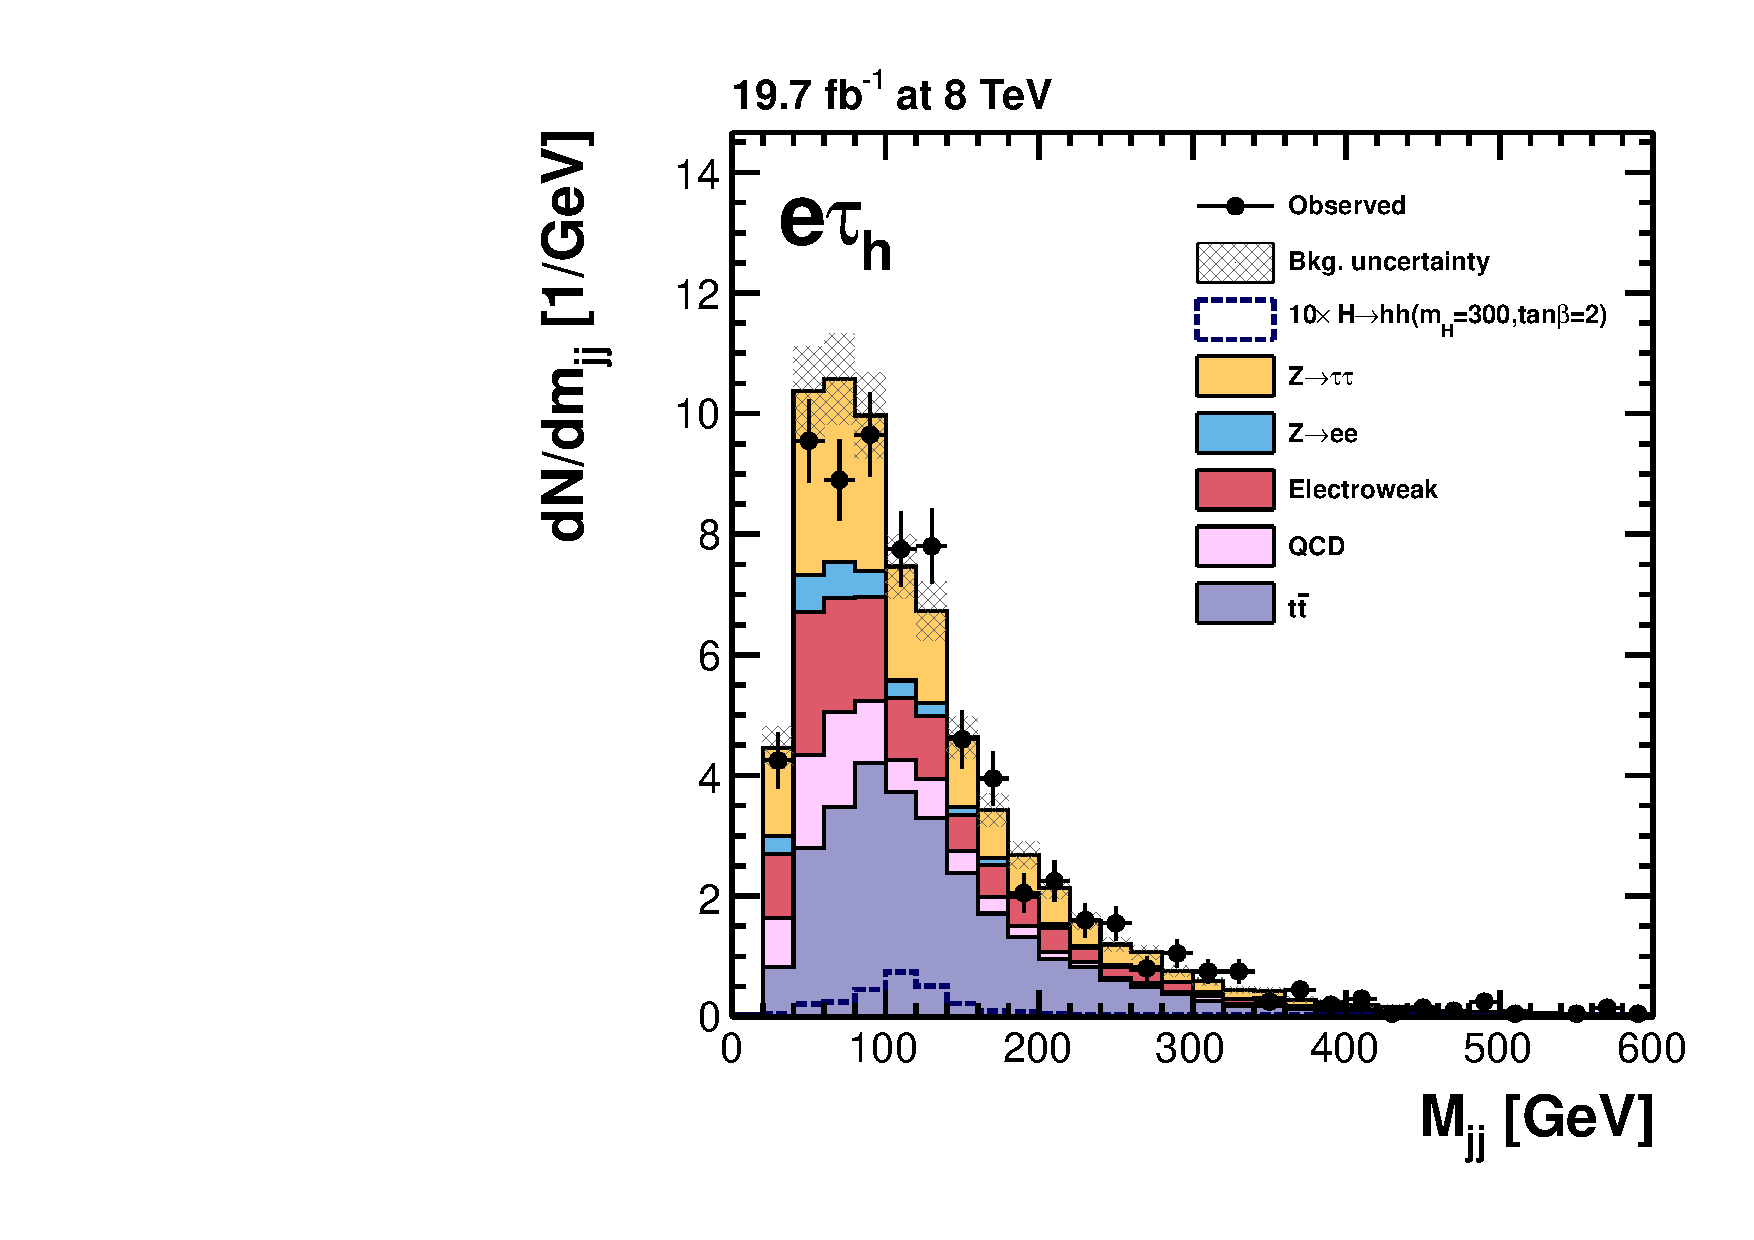
\includegraphics[width=0.5\textwidth] 
      {plots/Hhh/prebjet_mjj_2jet1tagSF_et_2012.pdf}} 
\end{center}
\caption[Distributions of $m_{\Pgt\Pgt}$ (left) and $m_{\Pqb\Pqb}$ (right) in the $\mutau$ (top) and
$\etau$ (bottom) channels for the 2jet--1tag category.]{
Distributions of $m_{\Pgt\Pgt}$ (left) and $m_{\Pqb\Pqb}$ (right) in the $\mutau$ (top) and
$\etau$ (bottom) channels for the 2jet--1tag category. The signal peaks close to
$125\,\GeV$ in both variables, motivating the application of cuts in a window
around $125\,\GeV$ to select the most signal-like events.}
\label{fig:2jet1tagmttmbb}
\end{figure} 

\begin{figure}
\begin{center}
\subfloat[]{
    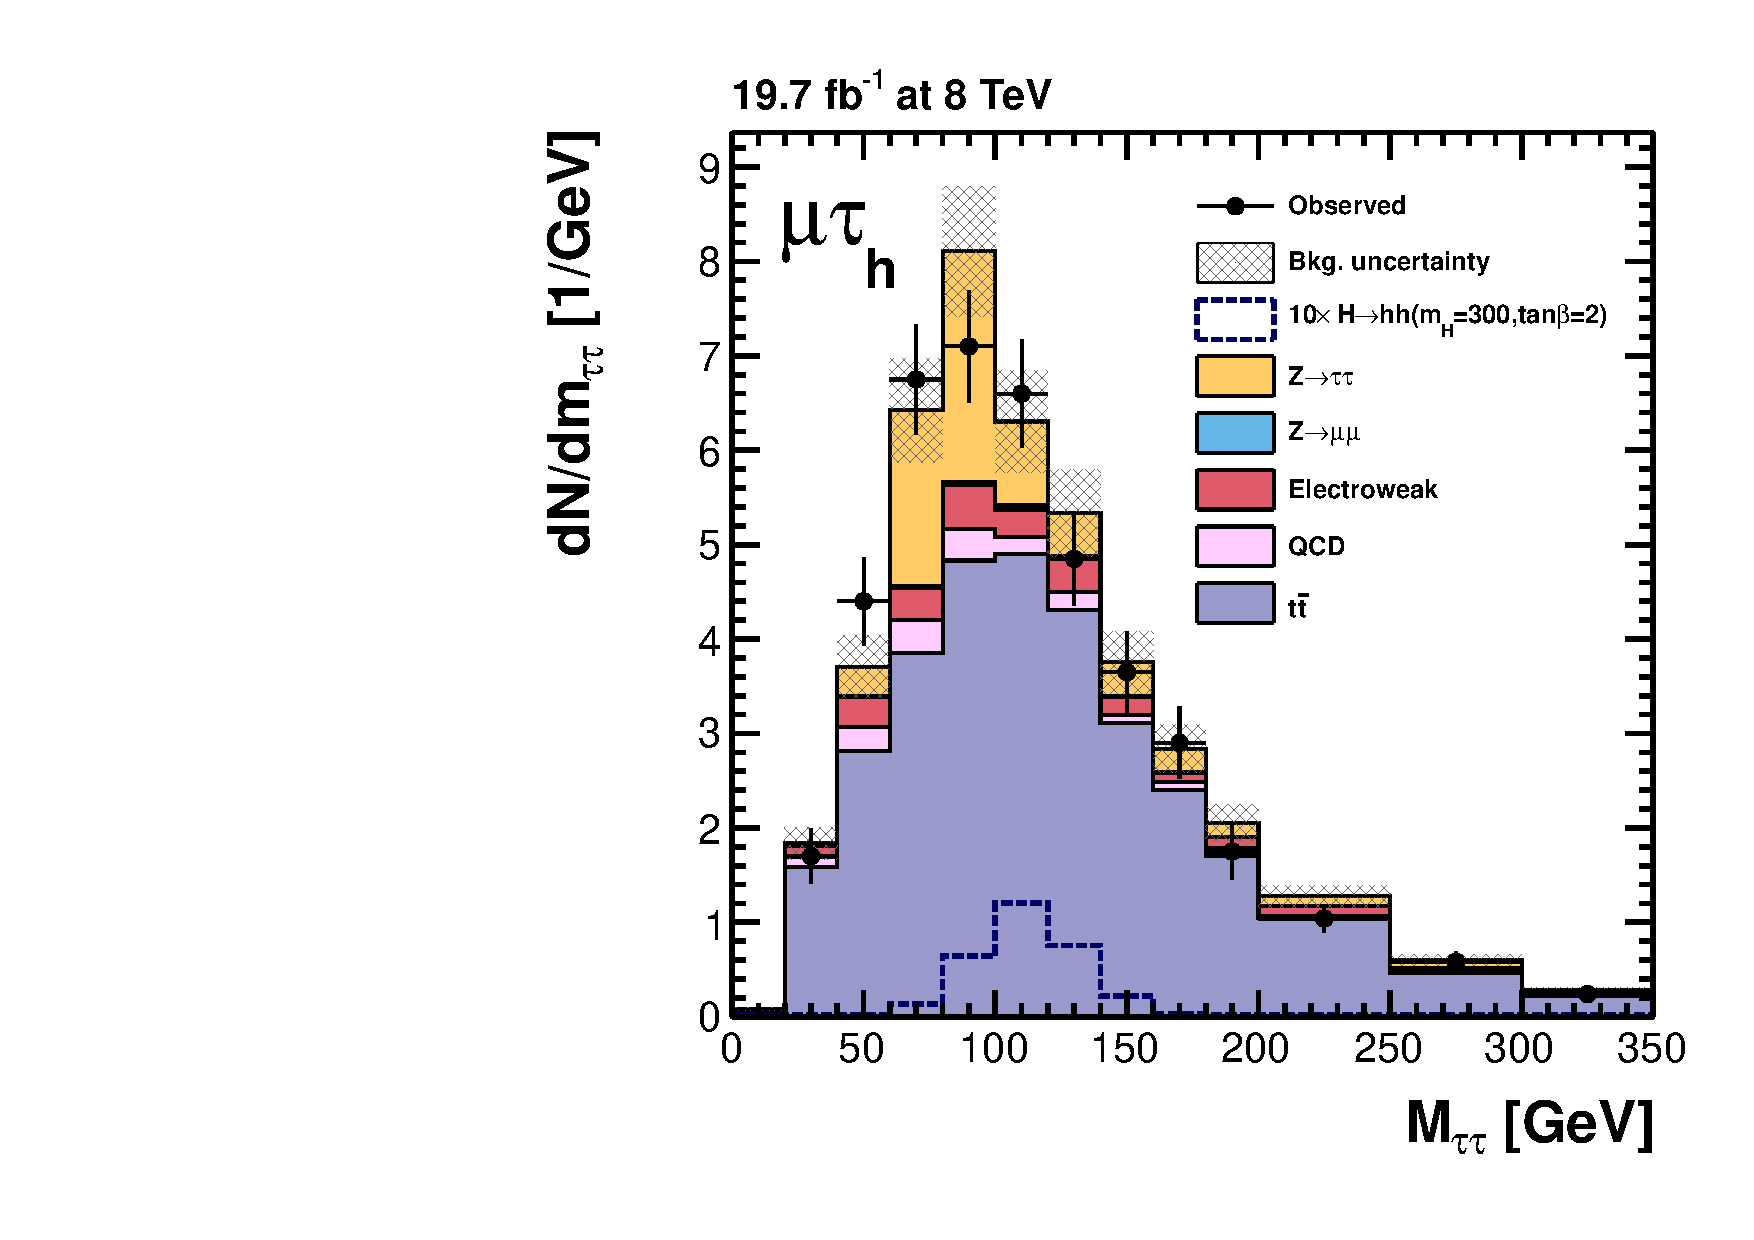
\includegraphics[width=0.5\textwidth]
      {plots/Hhh/m_sv_2jet2tagSF_mt_2012.pdf}}
\subfloat[]{
    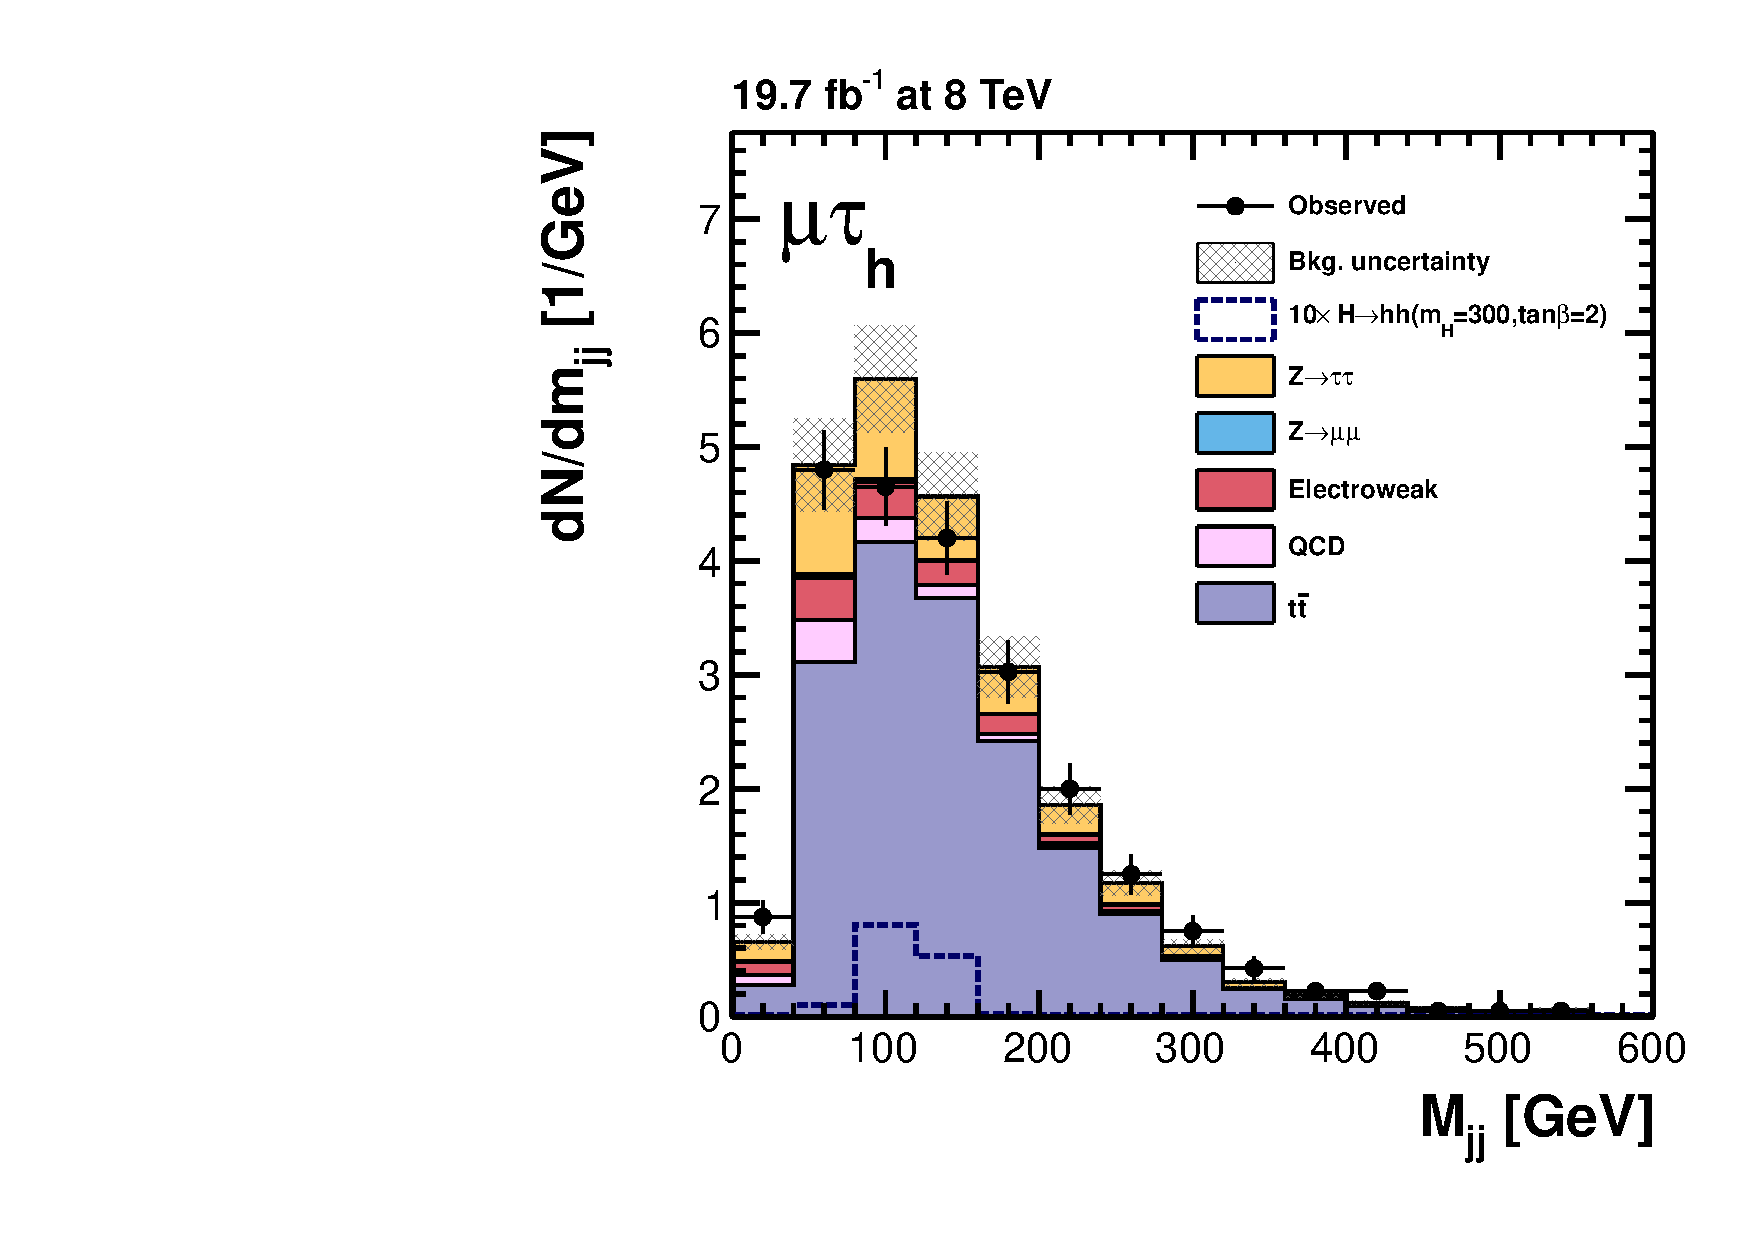
\includegraphics[width=0.5\textwidth] 
      {plots/Hhh/prebjet_mjj_2jet2tagSF_mt_2012.pdf}} 

\subfloat[]{
    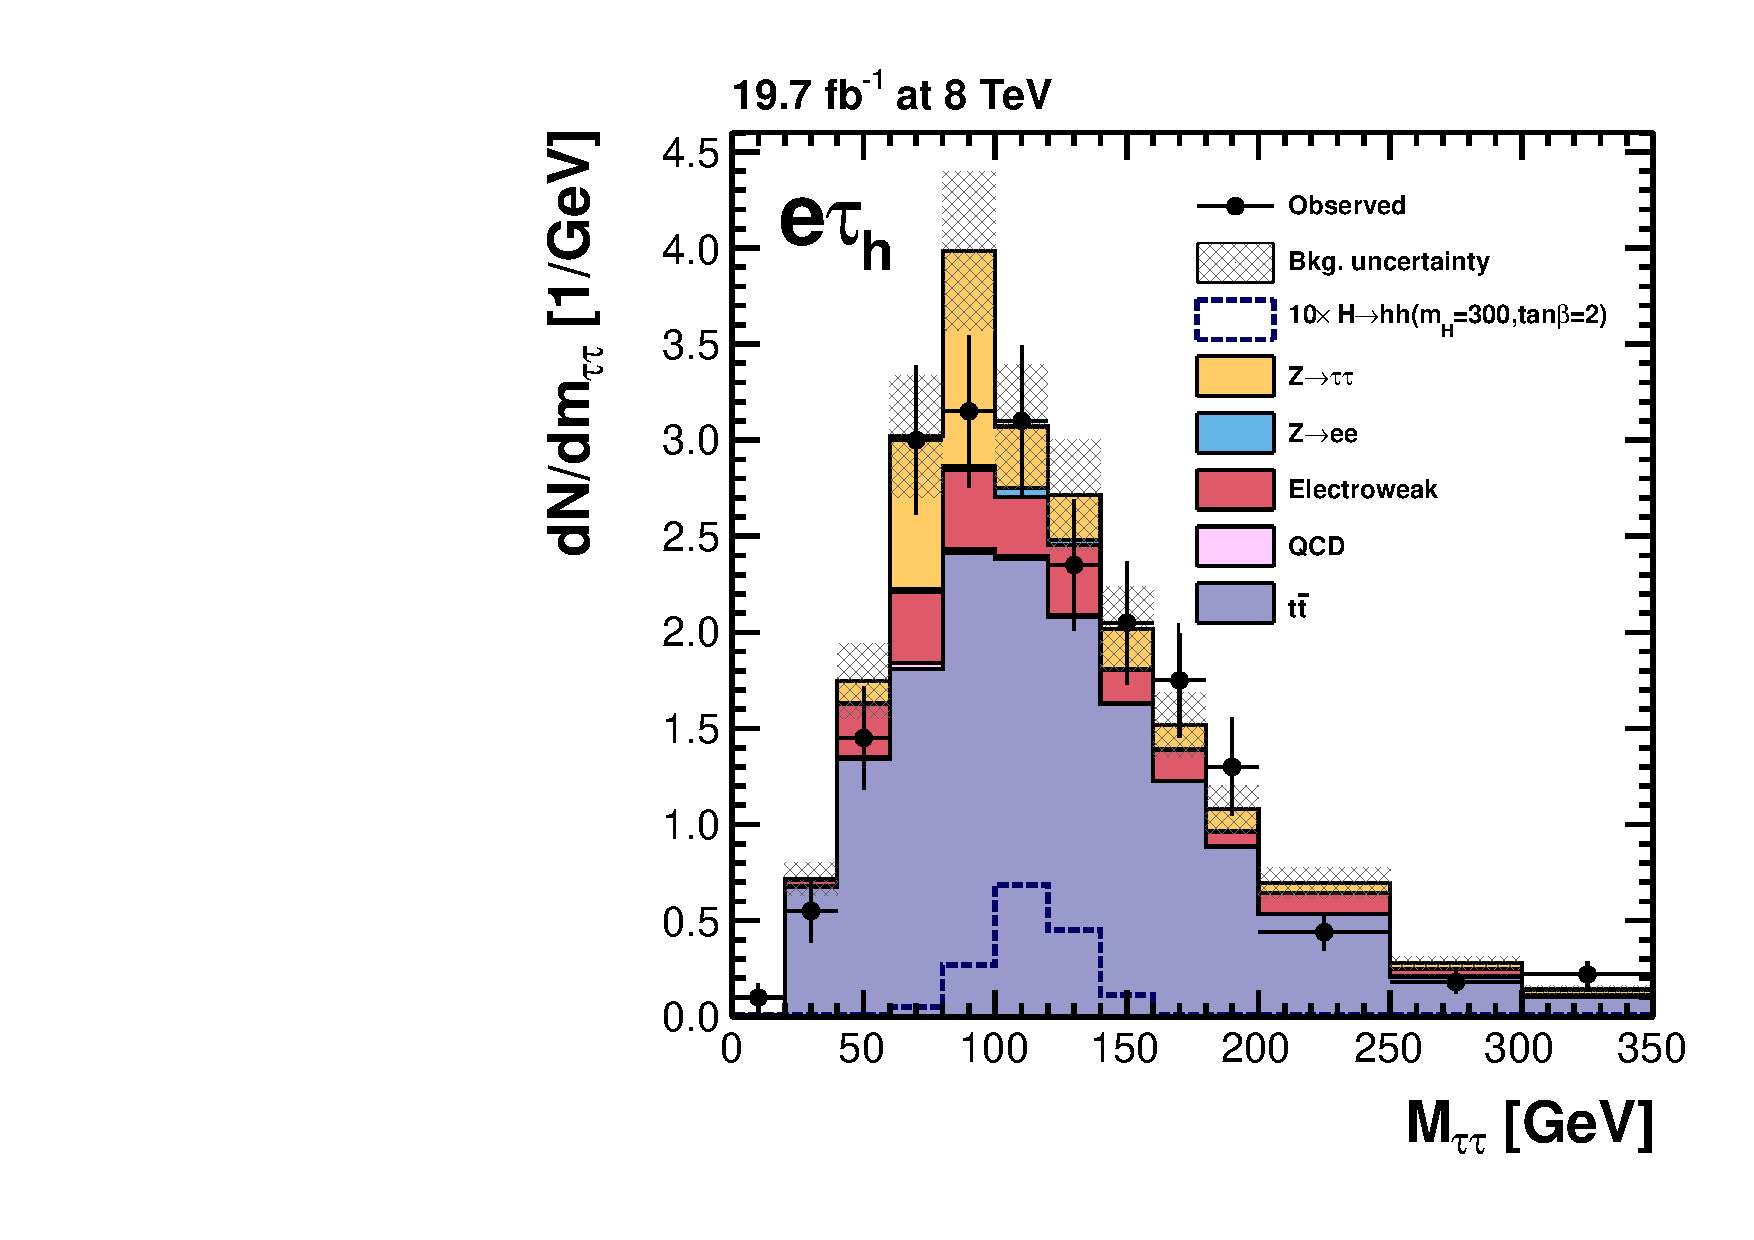
\includegraphics[width=0.5\textwidth]
      {plots/Hhh/m_sv_2jet2tagSF_et_2012.pdf}}
\subfloat[]{
    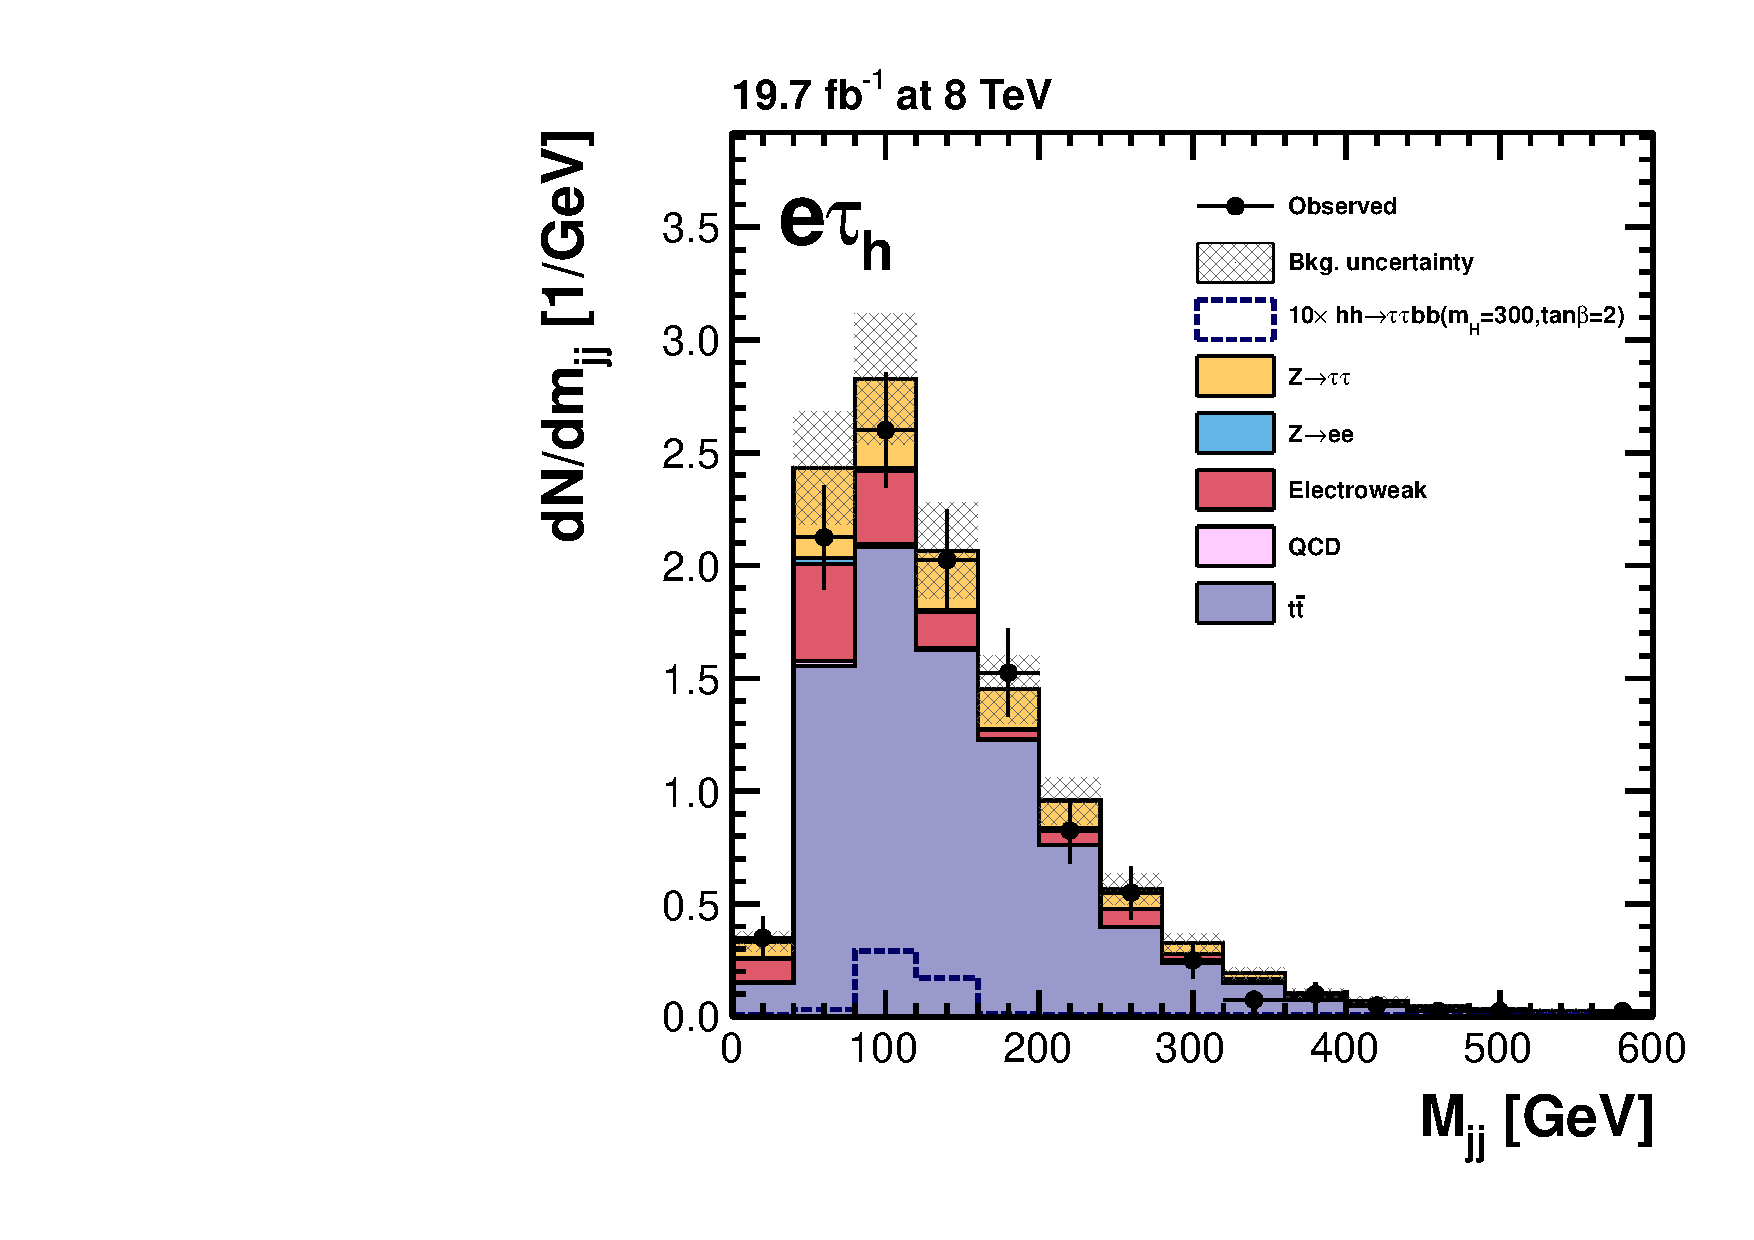
\includegraphics[width=0.5\textwidth] 
      {plots/Hhh/prebjet_mjj_2jet2tagSF_et_2012.pdf}} 
\end{center}
\caption[Distributions of $m_{\Pgt\Pgt}$ (left) and $m_{\Pqb\Pqb}$ (right) in the $\mutau$ (top) and
$\etau$ (bottom) channels for the 2jet--2tag category.]{
Distributions of $m_{\Pgt\Pgt}$ (left) and $m_{\Pqb\Pqb}$ (right) in the $\mutau$ (top) and
$\etau$ (bottom) channels for the 2jet--2tag category. The signal peaks close to
$125\,\GeV$ in both variables, motivating the application of cuts in a window
around $125\,\GeV$ to select the most signal-like events.}
\label{fig:2jet2tagmttmbb}
\end{figure} 

\section{Kinematic Fitting to extract $m_{\PH}$}
\label{sec:kinematicfit}

In addition to applying cuts on $m_{\Pqb\Pqb}$ and $m_{\Pgt\Pgt}$, the condition that
both values should be consistent with $125\,\GeV$ can be used further in
calculating the reconstructed heavy Higgs boson mass, $m_{\PH}$. This quantity can be reconstructed simply
by combining the visible taus, $\MET$ and the b-jets, denoted by $m_{\Pgt\Pgt+jj}$.
A better reconstruction is obtained by using the conditions on $m_{\Pqb\Pqb}$ and
$m_{\Pgt\Pgt}$ in a kinematic fit. 

In such a method, observables related to the
event kinematics are varied within their measurement uncertainties in order to
find the values which best fulfil a kinematic constraint. In this case, the
variables being varied correspond to the energies of the taus and b-jets and the
kinematic constraints are that $m_{\Pqb\Pqb} = m_{\Pgt\Pgt} = m_{\Ph} = 125\,\GeV$. 
Differences between the measured value and the constraint are accounted for in a cost
function $\chi^{2}$ which is minimised in the fitting procedure.  

For the b-jets, it is assumed that the reconstructed position in terms of the
angles $\eta$ and $\phi$ is known to great accuracy, and the largest
uncertainty is in the measurement of the energy. Thus in the fit only the
energy of the jets is varied and the position is kept constant. To first
approximation any uncertainty in energy directly translates to an uncertainty in
momentum related by the quantity $\vec{\beta} = \vec{p}/E$, which is assumed to be constant and 
not varied in the fit. The energy of the first b-jet is varied, and the
energy of the second b-jet can be related to the first using the following
kinematic conditions:

\begin{equation}
m_{\Ph}^{2} = \left( E_{\Pqb_{1}} + E_{\Pqb_{2}}^{\text{fit}} \right)^{2} -
\left(\vec{p}_{\Pqb_{1}} + \vec{p}_{\Pqb_{2}}^{\text{~fit}}\right)^{2} 
= m_{\Pqb_{1}}^{2} + \frac{E_{\Pqb_{2}}^{2,\text{fit}}}{\gamma_{\Pqb_{2}}^{2}} +
2E_{\Pqb_{1}}E_{\Pqb_{2}}^{\text{fit}}\left(\underbrace{1-\vec{\beta}_{\Pqb_{1}}\vec{\beta}_{\Pqb_{2}}}_{A}\right),   
\label{eq:bjetkinfit}         
\end{equation}

where $\gamma_{\Pqb_{1,2}} = 1/\sqrt{1-\vec{\beta}_{\Pqb_{1,2}}^{2}}$. The term $A$ is
assumed to be constant and hence can be derived from the pre-fit event
kinematics as:

\begin{equation}
A = \frac{m_{\Pqb_{1}\Pqb_{2}}^{2} - m_{\Pqb_{1}}^{2} - m_{\Pqb_{2}}^{2}}{2E_{\Pqb_{1}}E_{\Pqb_{2}}} , 
\end{equation}

which allows equation \ref{eq:bjetkinfit} to be reduced to:

\begin{equation}
E_{\Pqb_{2}}^{\text{fit}} = E_{\Pqb_{1}}A\gamma_{\Pqb_{2}}^{2}\left(-1 + \sqrt{1 +
\frac{m_{\Ph}^{2} -
m_{\Pqb_{1}^{2}}}{\left(E_{\Pqb_{1}}A\gamma_{\Pqb_{2}}\right)^{2}}}\right) .
\label{eq:bjetrelation}
\end{equation}

During the fitting procedure, the masses of the b-jets are allowed to scale
according to the ratio of the fitted energy:

\begin{equation}
m_{\Pqb_{1,2}}^{\text{fit}} = m_{\Pqb_{1,2}} \frac{E_{\Pqb_{1,2}}^{\text{fit}}}{E_{\Pqb_{1,2}}} 
\end{equation}

A $\chi^{2}$ quantity for each b-jet is constructed to quantify how much the fit has
modified the b-jet energy as:

\begin{equation}
\chi_{\Pqb_{1,2}}^{2} = \frac{E_{\Pqb_{1,2}}^{\text{fit}} -
E_{\Pqb_{1,2}}^{\text{meas}}}{\sigma_{\Pqb_{1,2}}}
\end{equation}

where $E_{\Pqb_{1,2}}^{\text{meas}}$ is the measured b-jet energy and $\sigma_{\Pqb_{1,2}}$
is the b-jet energy resolution. The value of $\sigma_{\Pqb_{1,2}}$ is estimated
using a \ac{MC} sample in different bins of $\eta$ and $\pt$ \cite{Schlieckau}. 

The taus are treated in a slightly different way in the fit due to the $\MET$
associated with their decays. It is assumed that the collinear approximation
holds such that the visible products are produced in the same direction as the
original tau. This direction is assumed to be known to a high degree of
accuracy, as in the case of the b-jets, and so is not varied in the fit. Thus 
only the energy of one tau is free in the fit, and
the energy of the other tau can be related to the first analogously to 
equation \ref{eq:bjetrelation}. The mass of either tau lepton is kept
constant at $m_{\Pgt}$.  

In order to find the correct tau energies, additional constraints are put on
the event using the $\MET$ to enforce that the heavy Higgs boson recoil from the fit
is close to the reconstructed recoil. The recoil from the fit can be defined as:
%check this equation - should they all be p_T?
\begin{equation}
\vec{p}_{\text{T},\text{recoil}}^{\text{~fit}} = -
\vec{p}_{\text{T},\Pqb_{1}}^{\text{~fit}} -
\vec{p}_{\text{T},\Pqb_{2}}^{\text{~fit}} -
\vec{p}_{\text{T},\Pgt_{1}}^{\text{~fit}} - \vec{p}_{\text{T},\Pgt_{2}}^{\text{~fit}} = -
\vec{p}_{\text{T},\text{H}}^{\text{~fit}} ,
\end{equation}

and the measured recoil as:

\begin{equation}
\vec{p}_{\text{T},\text{recoil}}^{\text{~meas}} = -
\vec{p}_{\text{T},\text{miss}}^{\text{~meas}} -
\vec{p}_{\text{T},\Pqb_{1}}^{\text{~meas}} - \vec{p}_{\text{T},\Pqb_{2}}^{\text{~meas}} -
\vec{p}_{\text{T},\Pgt_{1}^{\text{vis}}}^{\text{~meas}} -
\vec{p}_{\text{T},\Pgt_{2}^{\text{vis}}}^{\text{~meas}} = -
\vec{p}_{\text{T},\text{H}}^{\text{~meas}} ,
\end{equation}

where $\vec{p}_{\text{T},\text{miss}}^{\text{~meas}}$ is the vector of the
reconstructed $\MET$. The $\chi^{2}$ term corresponding to the agreement between these two quantities
can be constructed as:

\begin{equation}
\chi_{\text{recoil}}^{2} = \vec{p}_{\text{T},\text{recoil}}^{\text{~res},\text{T}} \cdot
\text{V}_{\text{recoil}}^{-1} \cdot
\vec{p}_{\text{T},\text{recoil}}^{\text{~res}} ,  
\end{equation}

where $\vec{p}_{\text{T},\text{recoil}}^{\text{~res}}$ is the residuum vector between
$\vec{p}_{\text{T},\text{recoil}}^{\text{~fit}}$
and $\vec{p}_{\text{T},\text{recoil}}^{\text{~meas}}$, and
$\vec{p}_{\text{T},\text{recoil}}^{\text{~res},\text{T}}$ indicates the
transpose. The covariance matrix of the recoil vector is estimated from
the covariance matrix of the $\vec{p}_{\text{T},\text{miss}}$ and the uncertainties of the b-jets as
follows:

\begin{equation}
\text{V}_{\text{recoil}} = \text{V}_{\vec{p}_{\text{T},\text{miss}}} - \text{V}_{\Pqb_{1}} -
\text{V}_{\Pqb_{2}} .
\end{equation}

The covariance matrices of the b-jets can be expressed entirely in terms of the
b-jet energy/momentum and position. Hence with inputs of the values and
covariance matrix of the missing transverse momentum (which comes directly from
MVA $\MET$) this component of the $\chi^{2}$ is entirely specified. 

The total $\chi^{2}$ to be minimised by the fit is then given by:

\begin{equation}
\chi_{\text{total}}^{2} = \chi_{\Pqb_{1}}^{2} + \chi_{\Pqb_{2}}^{2} + \chi_{\text{recoil}}^{2},
\end{equation}

which is a two dimensional function in variables $E_{\Pqb_{1}}$ and $E_{\Pgt_{1}}$.

The output of the kinematic fit is the 4-vector of each of the taus and b-jets,
with the energy and momentum corrected by the result of the fit. These 4-vectors
can be combined to yield the 4-body mass of the candidate $m_{\PH}$. Figure
\ref{fig:kinfitvsmttbb}
shows the difference between the heavy Higgs boson mass as reconstructed with and
without the kinematic fit for signal events with $m_{\PH}=300\,\GeV$. It can
be seen that both the mean and resolution of the reconstructed $m_{\PH}$ 
is greatly improved by the kinematic fit. Figure \ref{fig:kinfitsignalmasses} shows the
$m_{\PH}$ distribution with the kinematic fit (denoted $m_{\PH}^{\text{kinfit}}$) 
for different signal mass hypotheses in the range
considered for this analysis, using the example points of $m_{\PH}=260$, $300$ 
and $350\,\GeV$. From this figure it can be seen that the 4-body mass from the kinematic fit provides
good discrimination between the different mass hypotheses, such that in the
event of an excess of events in data, it would provide a good variable to make a prediction for
the most likely $m_{\PH}$ consistent with the data. This is not true, for example, 
in variables such as $m_{\Pgt\Pgt}$ and $m_{\Pqb\Pqb}$ where the signal looks very 
similar with a peak at $125\,\GeV$ for all $m_{\PH}$ hypotheses.

\begin{figure}
\begin{center}
    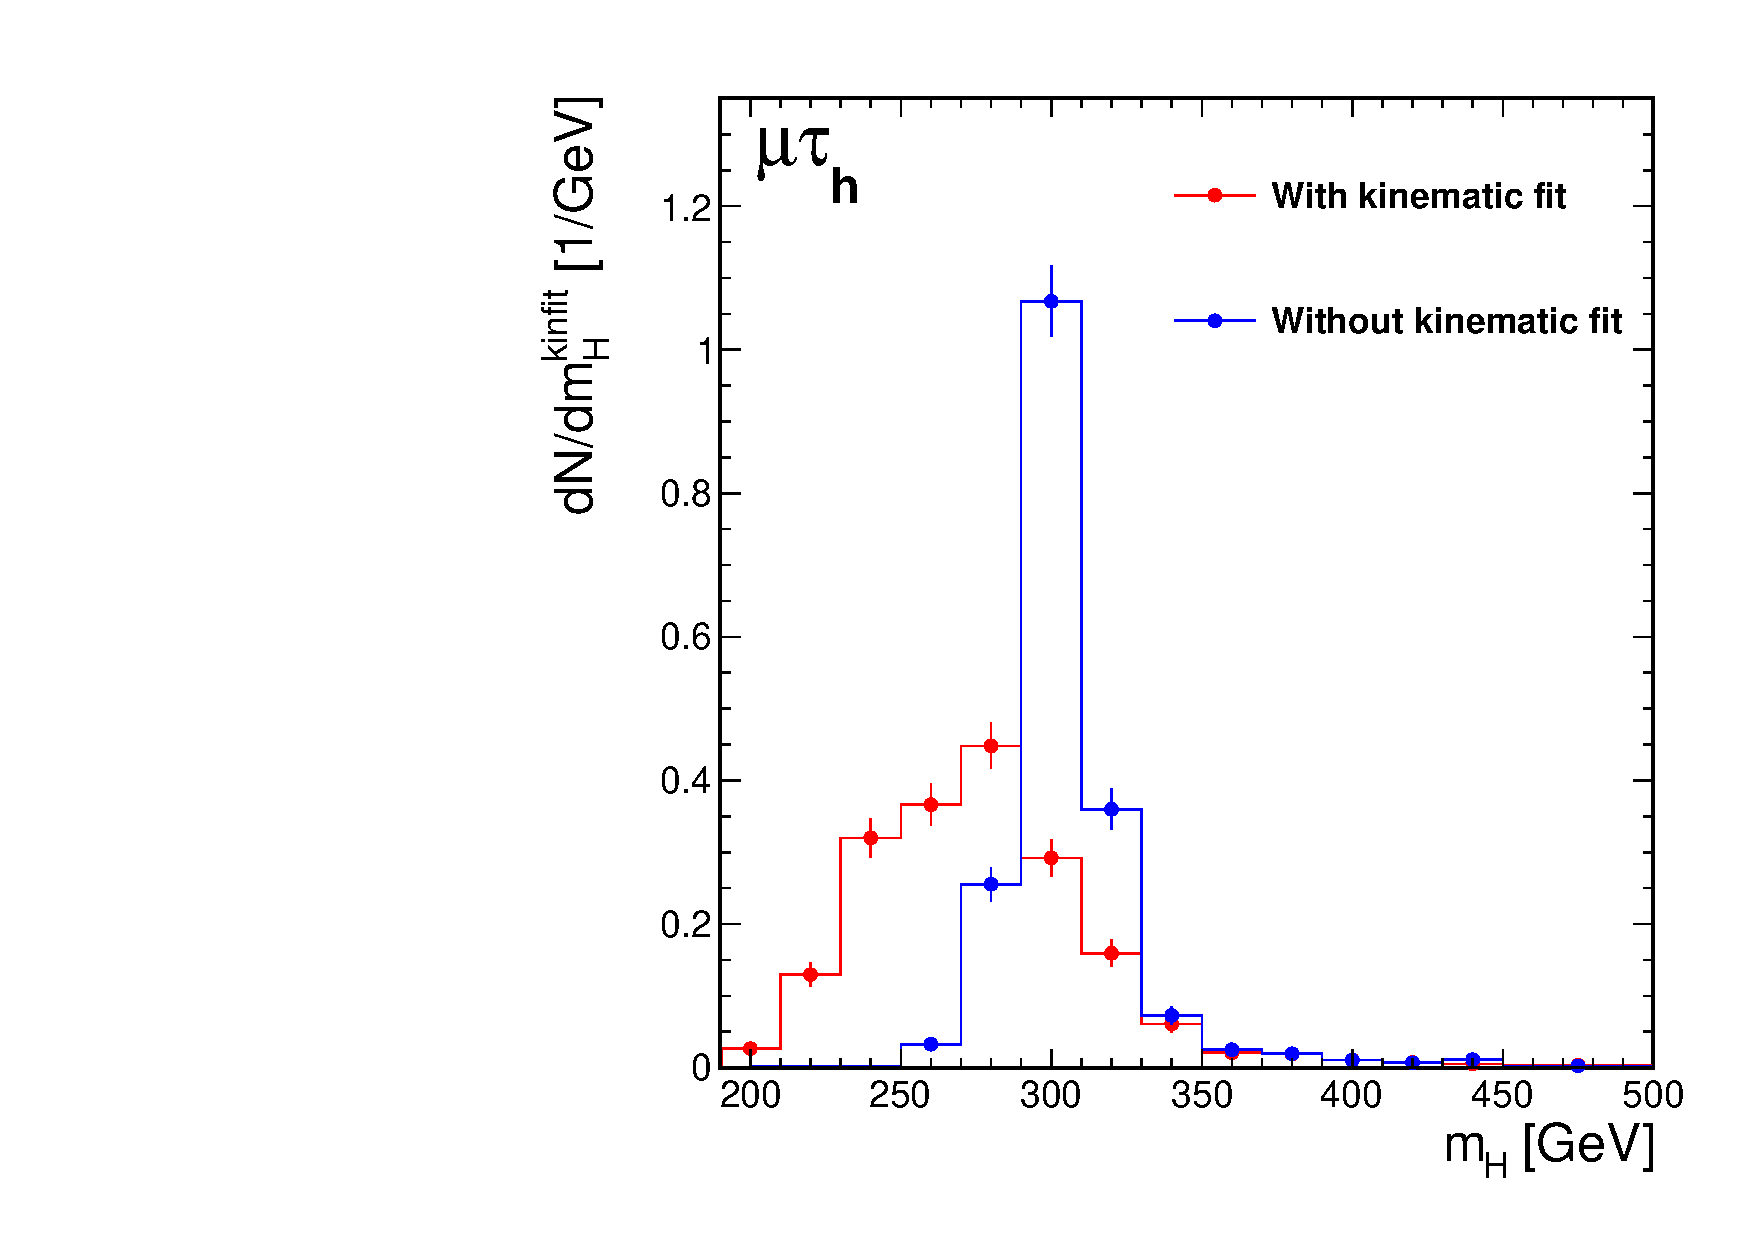
\includegraphics[width=0.5\textwidth]
      {plots/Hhh/m_H_kinfit_vs_mttbb_2jet2tagSFMassCuts_mt_ggHTohh300.pdf}

\end{center}
\caption[Four body mass of the candidate \PH in $\PH\to\Ph\Ph$ signal events with
$m_{\PH}=300\,\GeV$, reconstructed with or without a kinematic fit.]{
Four body mass of the candidate \PH in $\PH\to\Ph\Ph$ signal events with
$m_{\PH}=300\,\GeV$, as reconstructed using a simple sum of the
individual components (without kinematic fit) or using a kinematic fit as
described in the text. Shown for events in the 2jet--2tag category of the
$\mutau$ channel.}
\label{fig:kinfitvsmttbb}
\end{figure} 

\begin{figure}
\begin{center}
    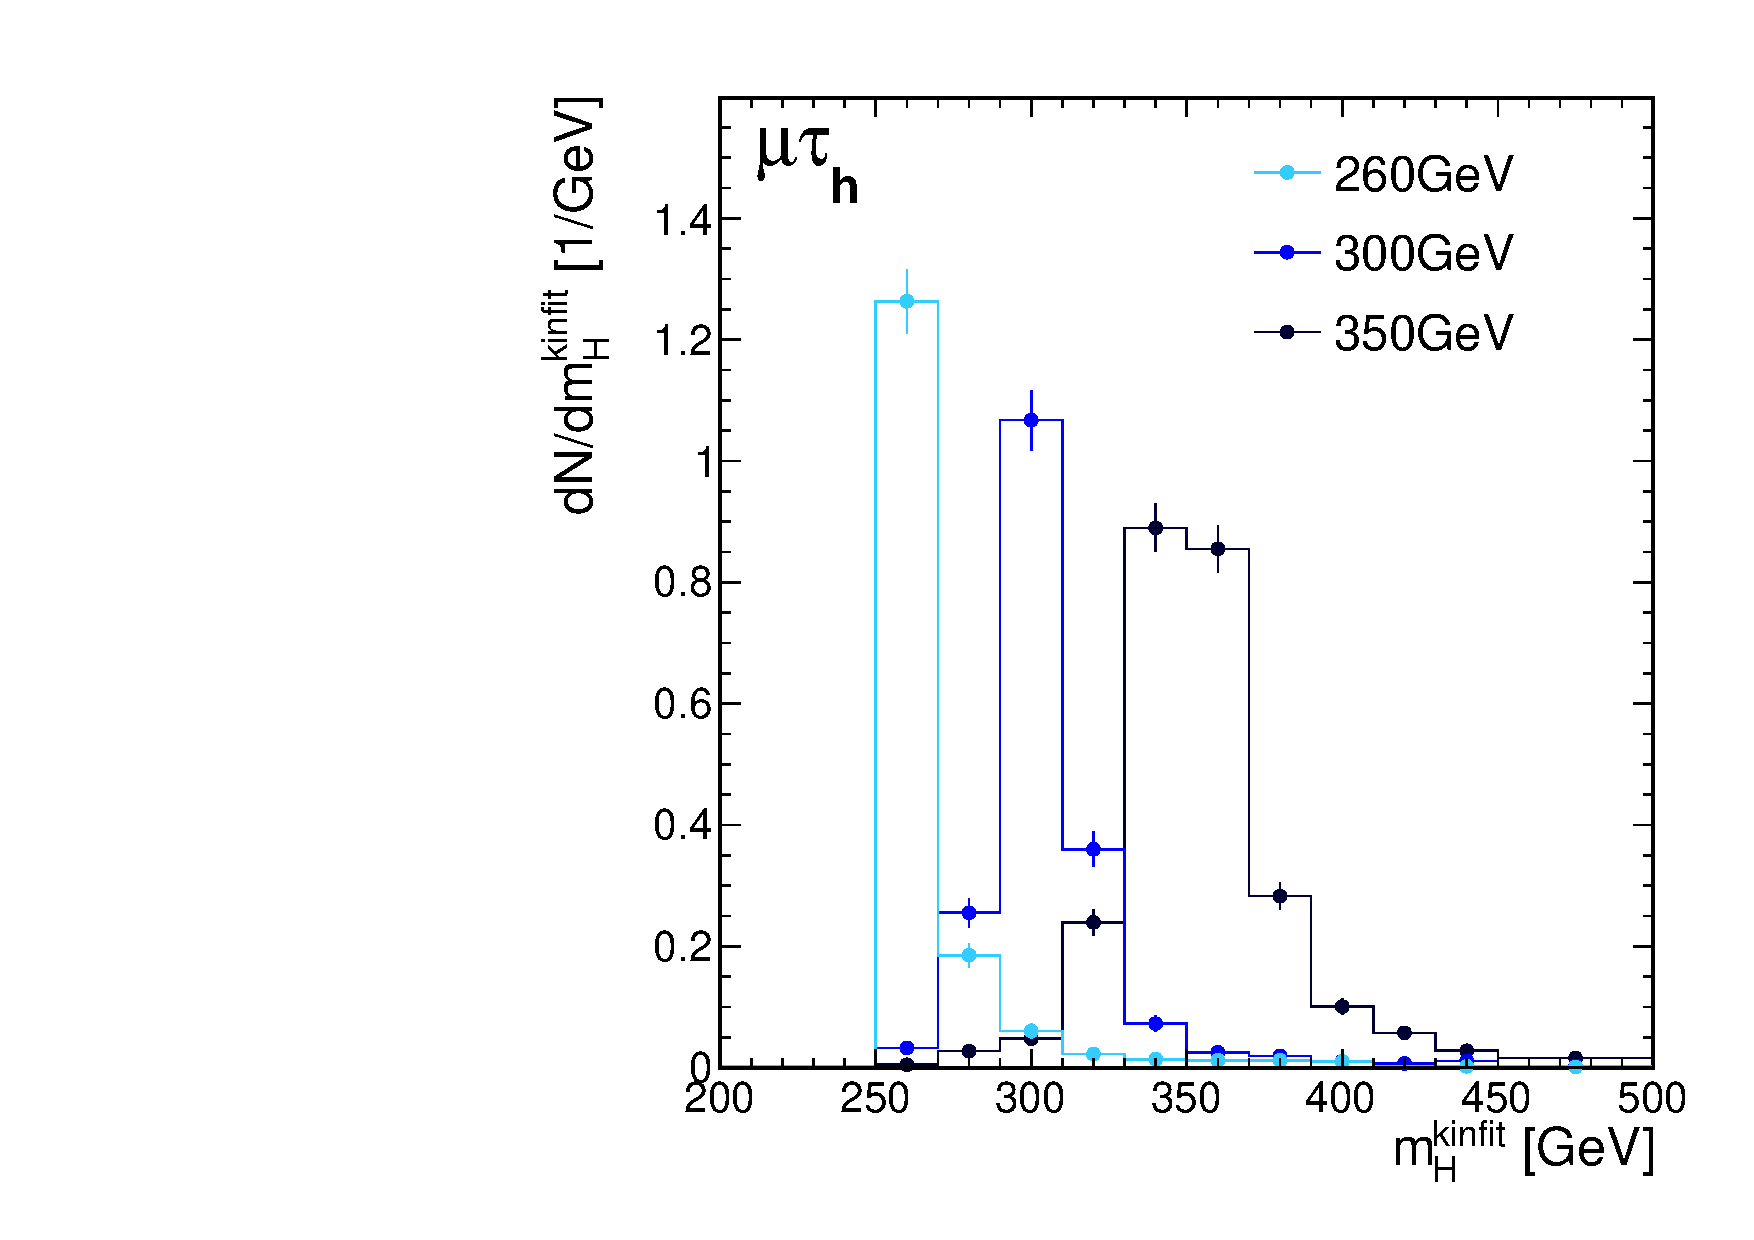
\includegraphics[width=0.5\textwidth]
      {plots/Hhh/m_H_kinfit_signalmasses_2jet2tagSFMassCuts_mt.pdf}

\end{center}
\caption[]{
Four body mass of the candidate \PH in $\PH\to\Ph\Ph$ signal events with
$m_{\PH}=260$, $300$ or $350\,\GeV$, as reconstructed using the kinematic fit}
\label{fig:kinfitsignalmasses}
\end{figure} 

Figure~\ref{fig:kinfitvsmttbbstacked} shows the effect of the kinematic
fit on the full distribution including all of the backgrounds and data, for the
example of events in the 2jet--1tag category. The shape of the backgrounds is
not altered greatly by the fit, with the exception of forcing a minimum at
$250\,\GeV$ due to the threshold for $2\times m_{\Ph}$, whereas the shape of
signal is greatly improved leading to much better shape discrimination between
signal and background. For this reason, the 4-body mass from the kinematic fit
is chosen as the discriminating variable for signal extraction.

\begin{figure}
\begin{center}
\subfloat[]{
    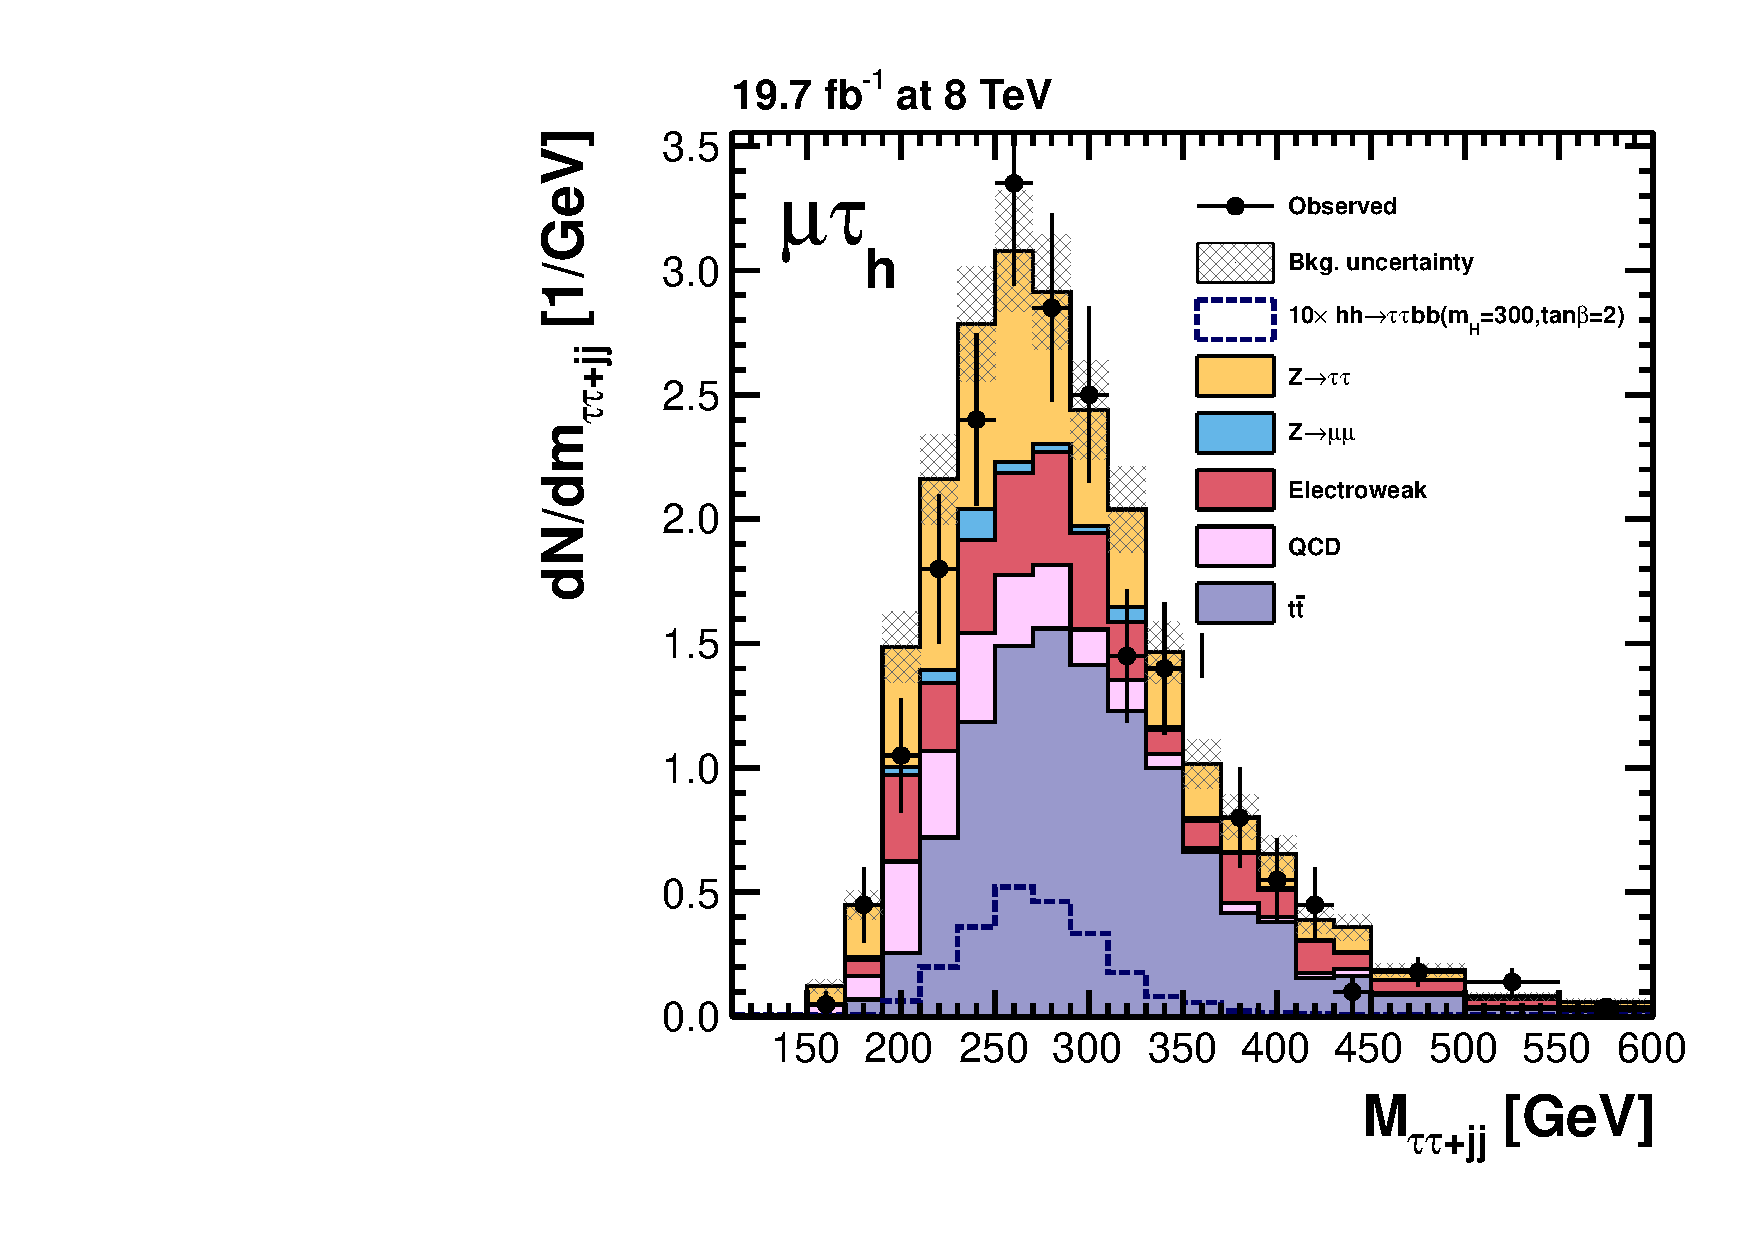
\includegraphics[width=0.5\textwidth]
      {plots/Hhh/mjj_tt_2jet1tagSFMassCuts_mt_2012.pdf}}
\subfloat[]{
    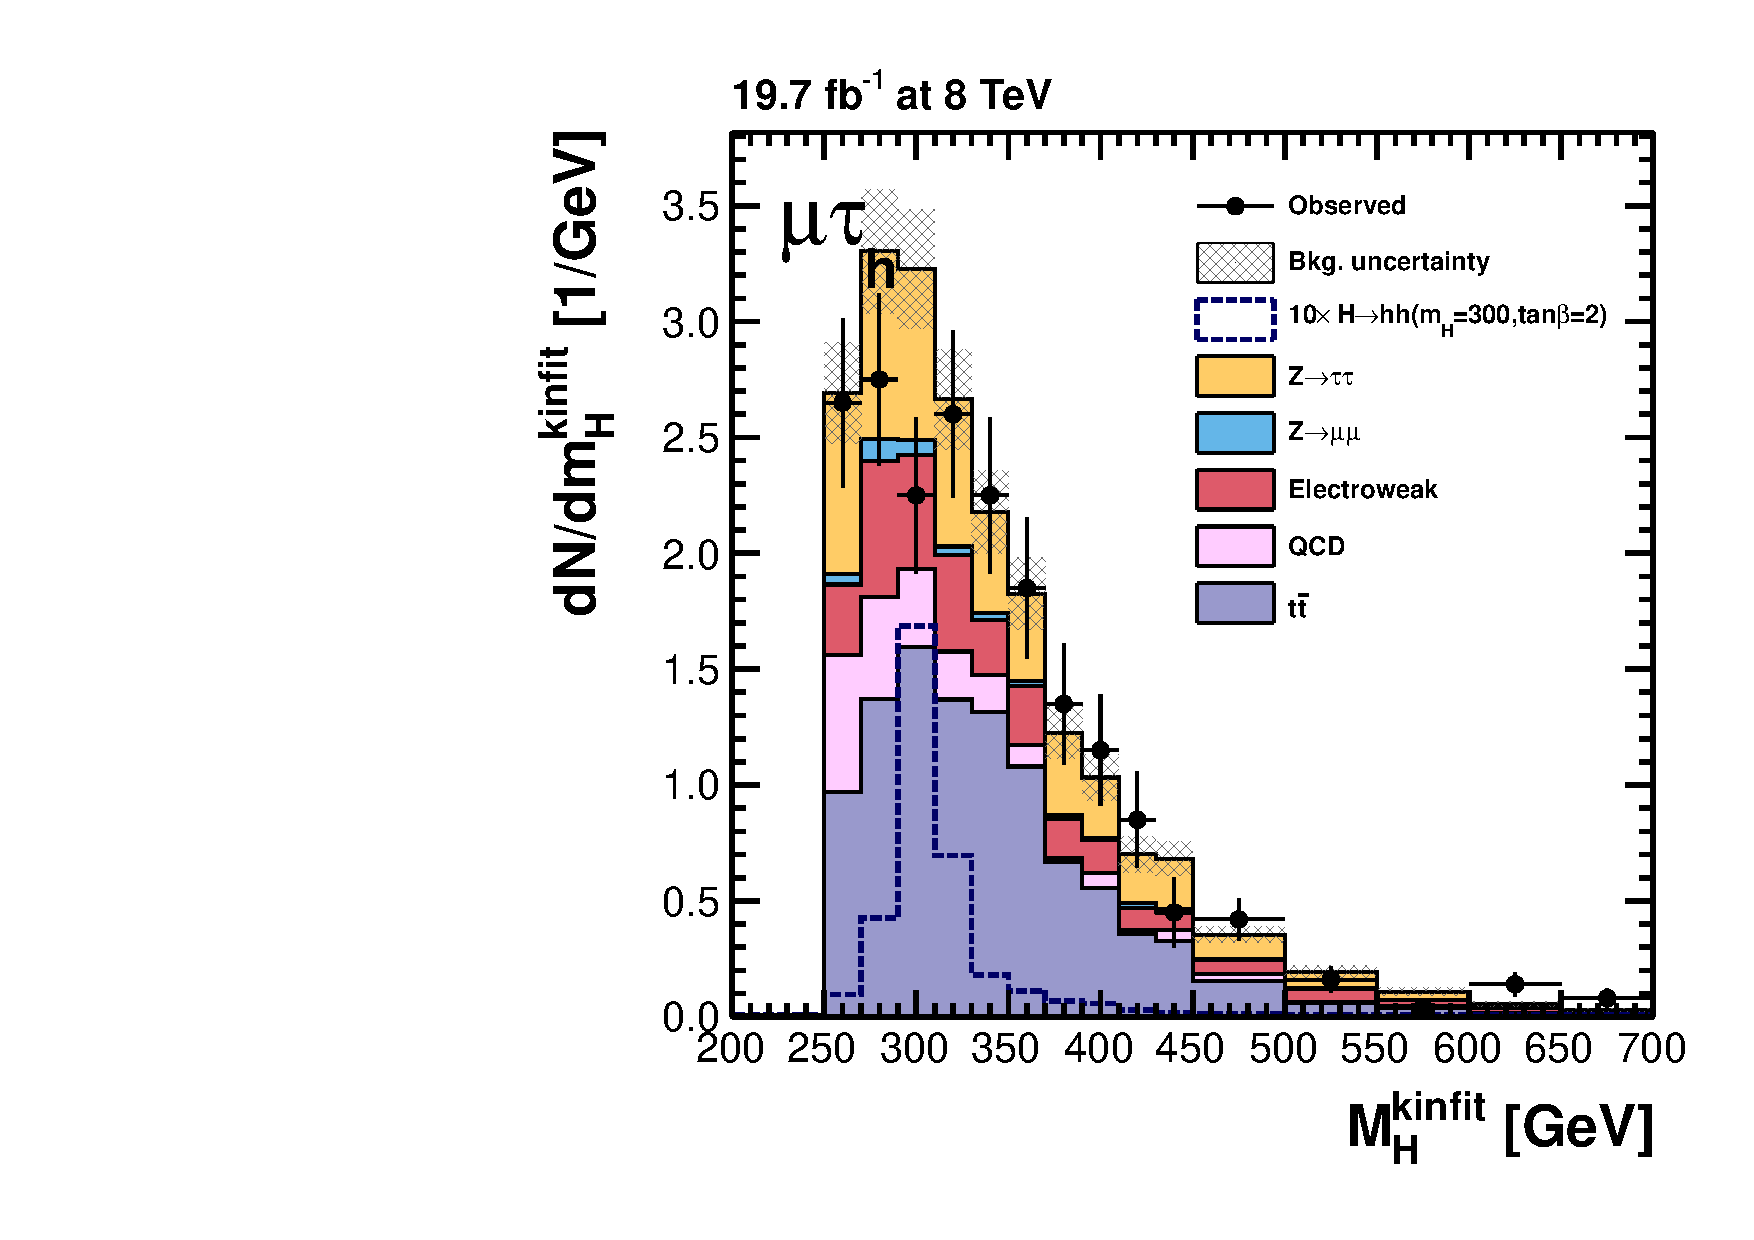
\includegraphics[width=0.5\textwidth]
      {plots/Hhh/m_H_hh_2jet1tagSFMassCuts_mt_2012.pdf}}

\end{center}
\caption[Four body mass of the candidate \PH in data and MC events reconstructed
with and without a kinematic fit.]{
Four body mass of the candidate \PH as reconstructed using a simple vector sum of the
individual components (a) and using a kinematic fit (b) as
described in the text. Shown for events in the 2jet--1tag category of the
$\mutau$ channel. The effect of the kinematic fit on the backgrounds is to force
a minimum at $2\times125=250\,\GeV$, but otherwise the shapes are largely
unchanged, while the shape of the signal is greatly improved.}
\label{fig:kinfitvsmttbbstacked}
\end{figure} 

\section{Datasets and MC samples}
\label{sec:Hhhdatasets}

The dataset used for this analysis corresponds to the complete 2012 dataset at
$\sqrt{s}=8\,\TeV$. Samples of background events correspond exactly to those
described in section~\ref{sec:dataandMC}. For the signal, \ac{MC} samples are
produced for $m_{\PH}$ masses between $260\,\GeV$ and $350\,\GeV$ in $10\,\GeV$
steps using \textsc{pythia}
for parton showering and hadronisation and \textsc{tauola}~\cite{TAUOLA} for tau
decays. Values for cross-section times branching ratio are calculated for the
low-$\tan\beta$-high scenario as described in section~\ref{sec:}.
For displaying the signal on figures, a benchmark point in this scenario is
chosen for illustration purposes.

\section{Background methods}
\label{sec:Hhhbackgrounds}

Inclusively, the background composition is the same as discussed in the previous
chapters. The additional requirement that the events contain at least two jets
changes the composition slightly, with the largest effect being an increase in
$\ttbar$ background and a decrease in $\ZToTauTau$, $\WJets$ and QCD. The
variation with category is large, with 2jet--0tag events containing mostly
$\ZToTauTau$, $\WJets$ and QCD, and 2jet--2tag events containing almost entirely
$\ttbar$. In general the background methods follow those described in the
previous chapters, with the exception of adaptations necessary to deal with the
increased amount of $\ttbar$ and the generally lower statistics in the
categories after applying the mass cuts on $m_{\Pqb\Pqb}$ and $m_{\Pgt\Pgt}$.

\subsection{$\ZToTauTau$}

The $\ZToTauTau$ background exists in the categories from $\PZ$ plus $\geq 2$
jet events. This is greatly reduced by the b-tagging requirements, and so most
events fall in the 2jet--0tag category. This component is also reduced somewhat
by the mass cut on $m_{\Pgt\Pgt}$, but the lower edge of the window at $90\,\GeV$
is such that the higher half of the $\ZToTauTau$ peak is still retained in the
signal region.  

As in the previous analyses, the $\ZToTauTau$ component is estimated using an
embedded sample. As in the \ac{MSSM} analysis, there is a known contamination in
this sample from $\ttbar$ events. This contribution is more important in this
analysis because there is no veto on events with more than one jet which
is applied in the b--tag category of the \ac{MSSM} analysis, and 
hence the analysis selects very $\ttbar$-like events,
especially in the 2jet--1tag and 2jet--2tag categories. The contribution is
estimated using a $\ttbar$ embedded sample as described in section
\ref{sec:mssmBackgrounds}. The contribution to the total normalisation is
approximately $10\%$ in 2jet--1tag and $27\%$ in 2jet--2tag. This is much larger
than in the \ac{MSSM} analysis, and so a more careful method is used to subtract
this contribution to avoid double counting. Instead of simply reducing the yield
of the $\ttbar$ prediction to account for this, the normalised shape of the
embedded $\ttbar$ is subtracted from the $\ZToTauTau$ estimate.

\subsection{$\ttbar$}

For the estimate of the large $\ttbar$ background, both shape and normalisation
are taken from \ac{MC}. As this background is so large in this analysis, it
is extremely important that this estimate is accurate. To improve the confidence
in this estimate, both shape and normalisation are checked against a data
control region. In the \ac{SM} and \ac{MSSM} $\HToTauTau$ analyses, this is done
using events in the $\emu$ final state, and the crucial distributions to check
the shapes os are mostly related to the taus, in particular $m_{\Pgt\Pgt}$. In this
analysis we are also concerned that the b-jets are well modelled in the
$\ttbar$ \ac{MC}. Since the $\emu$ final state is not actually used for this
analysis, it is also important to check $\mutau$ and $\etau$ events.
Hence two $\ttbar$ control regions are defined: the first is the same as is used
in the \ac{SM} and \ac{MSSM} $\HToTauTau$ analyses using the $\emu$ channel, 
and takes events with at least two jets, at least one b-tagged jet and
$\MET>80\,\GeV$. The second is defined using the
$\mutau$ final state and uses events with at least two b-tagged jets and in the
high $m_{\text{T}}>100\,\GeV$ region. Both control regions have purity in
$\ttbar$ events of larger than $90\%$. Figure~\ref{fig:ttbarcontrol} shows
distributions made in these control regions for the example distribution of the
leading and subleading b-jet $\pt$. There are no obvious differences in shape or
normalisation between the data and the \ac{MC} in these, or any of the other
distributions the analysis is sensitive to.

\begin{figure}
\begin{center}
\subfloat[]{
    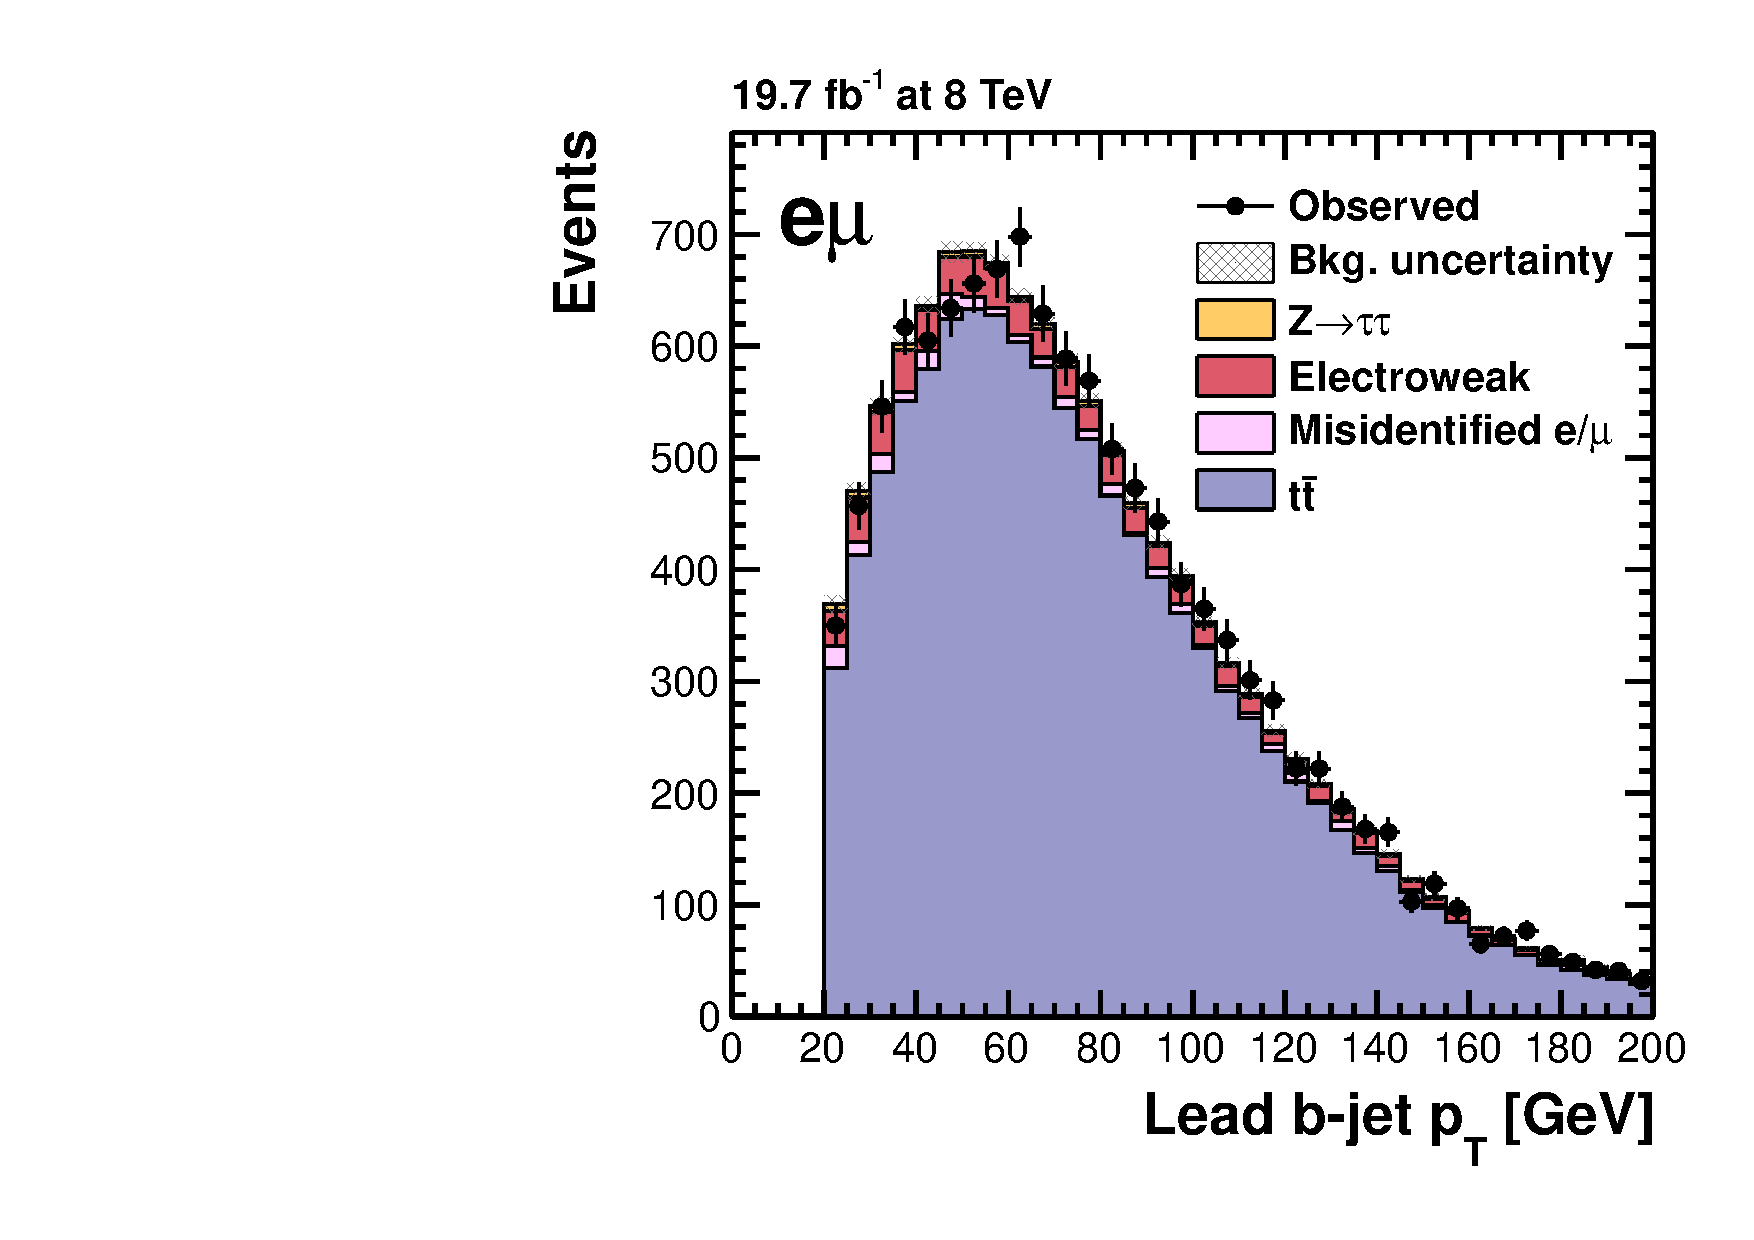
\includegraphics[width=0.5\textwidth]
      {plots/Hhh/TTBarControl/prebjetpt_1_2jetGT1tagSF_em_2012.pdf}}
\subfloat[]{
    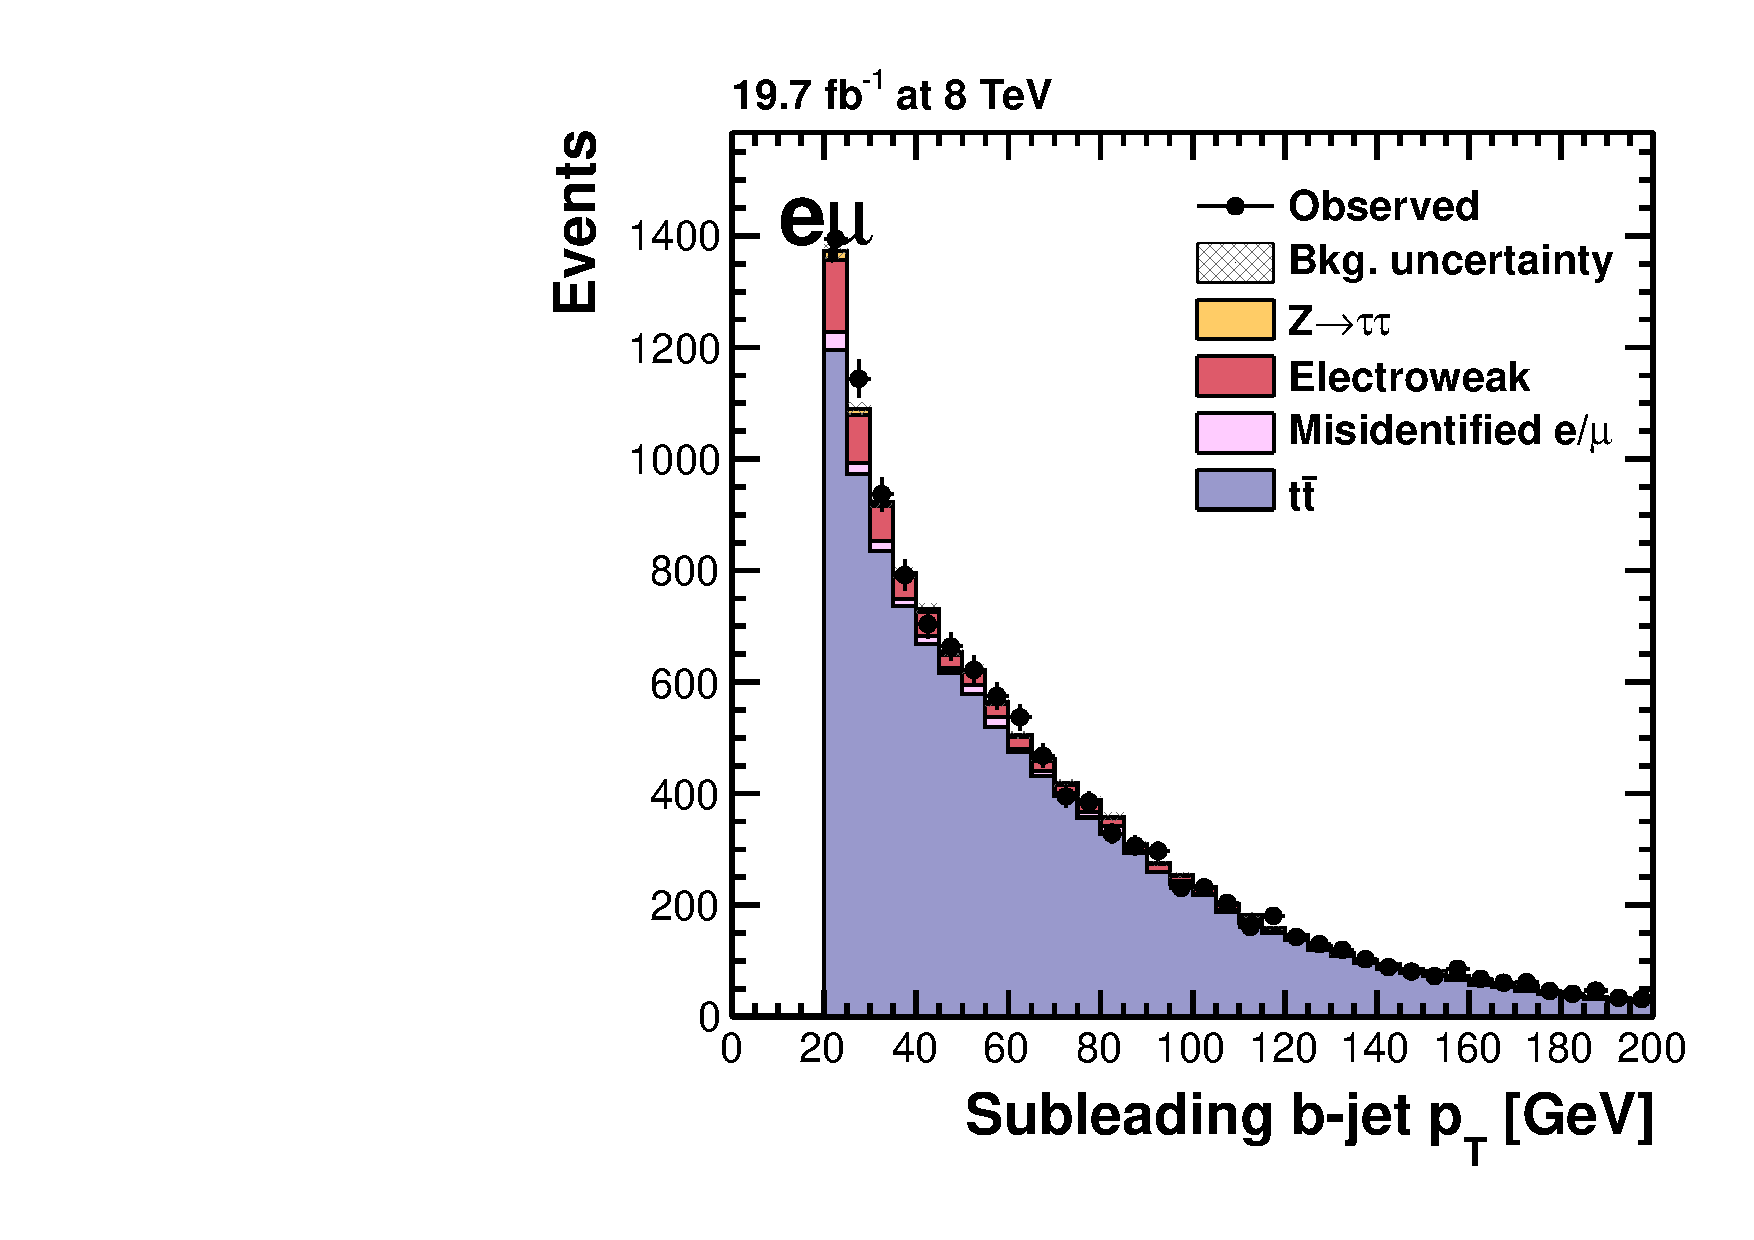
\includegraphics[width=0.5\textwidth]
      {plots/Hhh/TTBarControl/prebjetpt_2_2jetGT1tagSF_em_2012.pdf}}

\subfloat[]{
    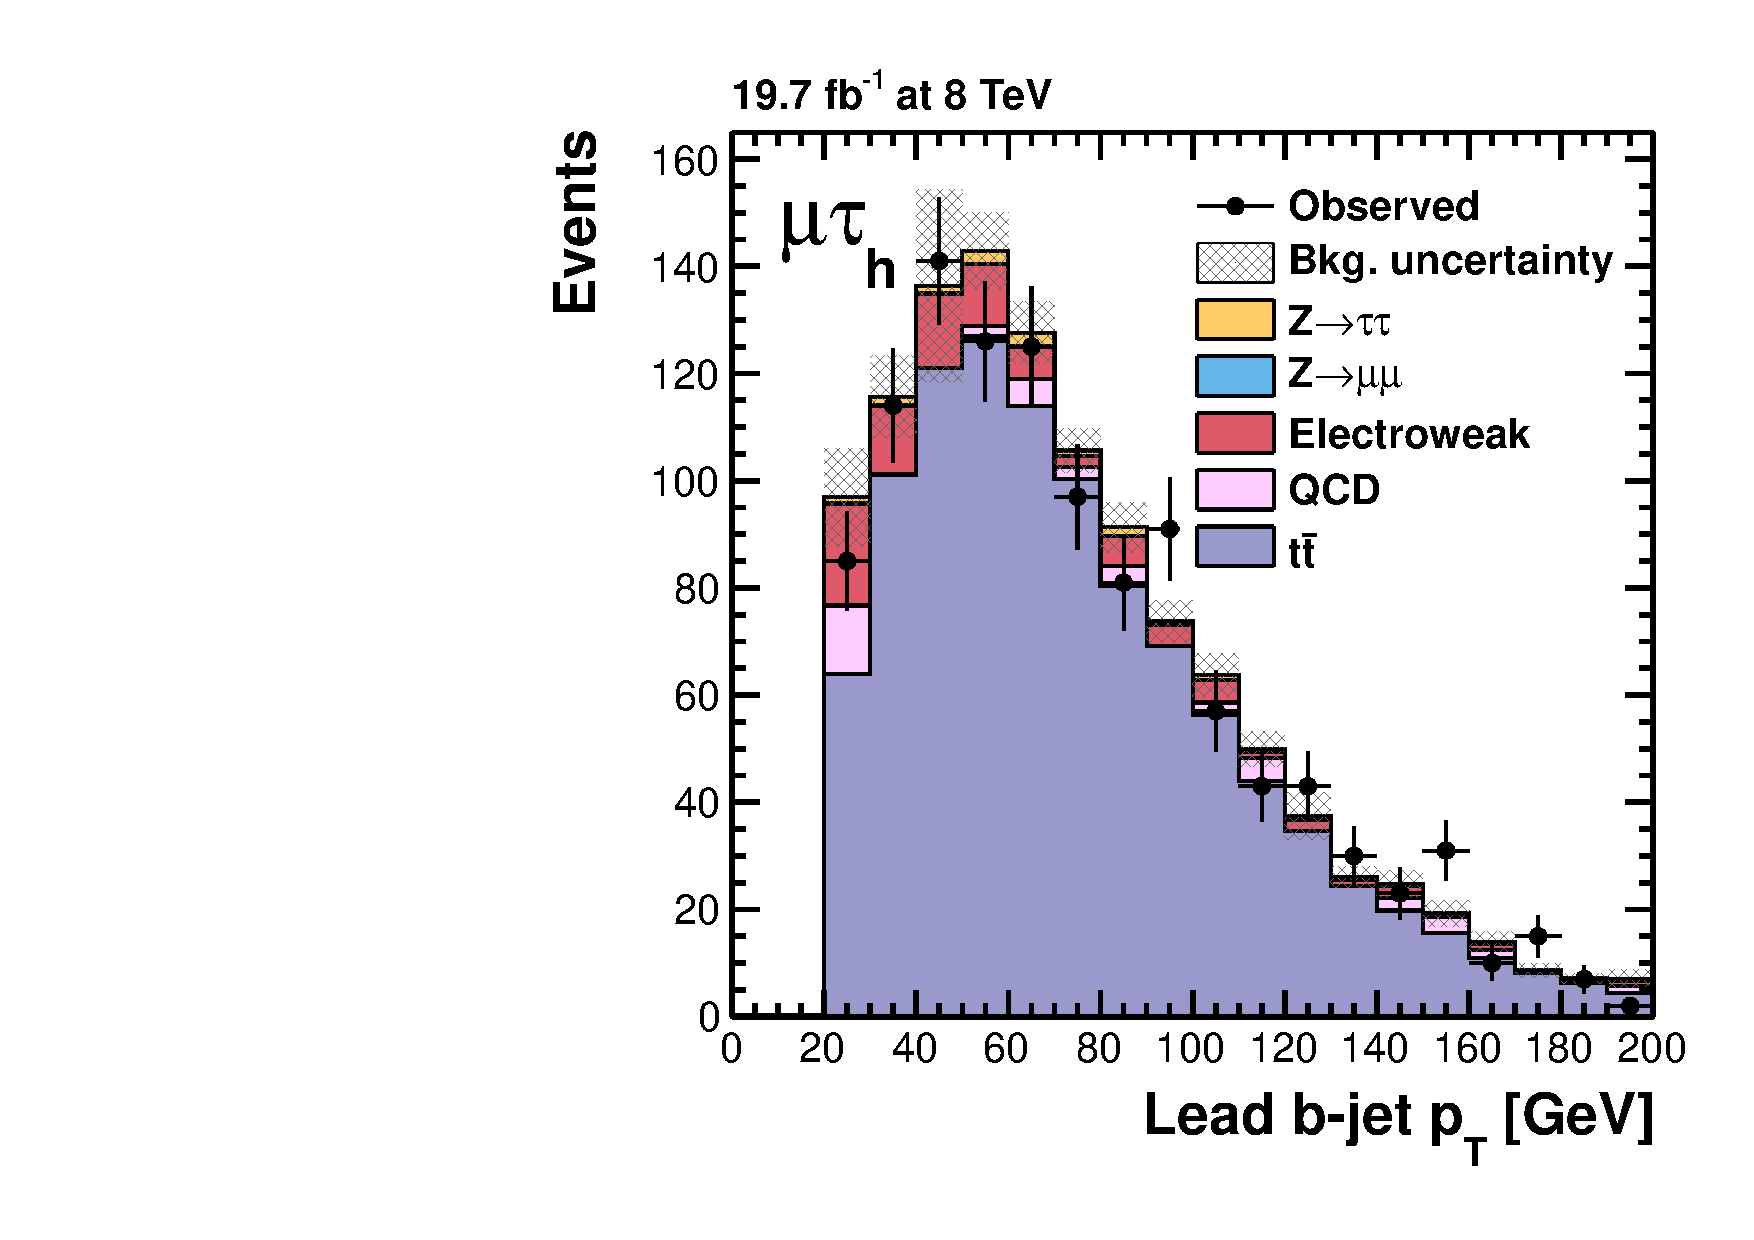
\includegraphics[width=0.5\textwidth]
      {plots/Hhh/TTBarControl/prebjetpt_1_2jet2tagSF_mt_2012.pdf}}
\subfloat[]{
    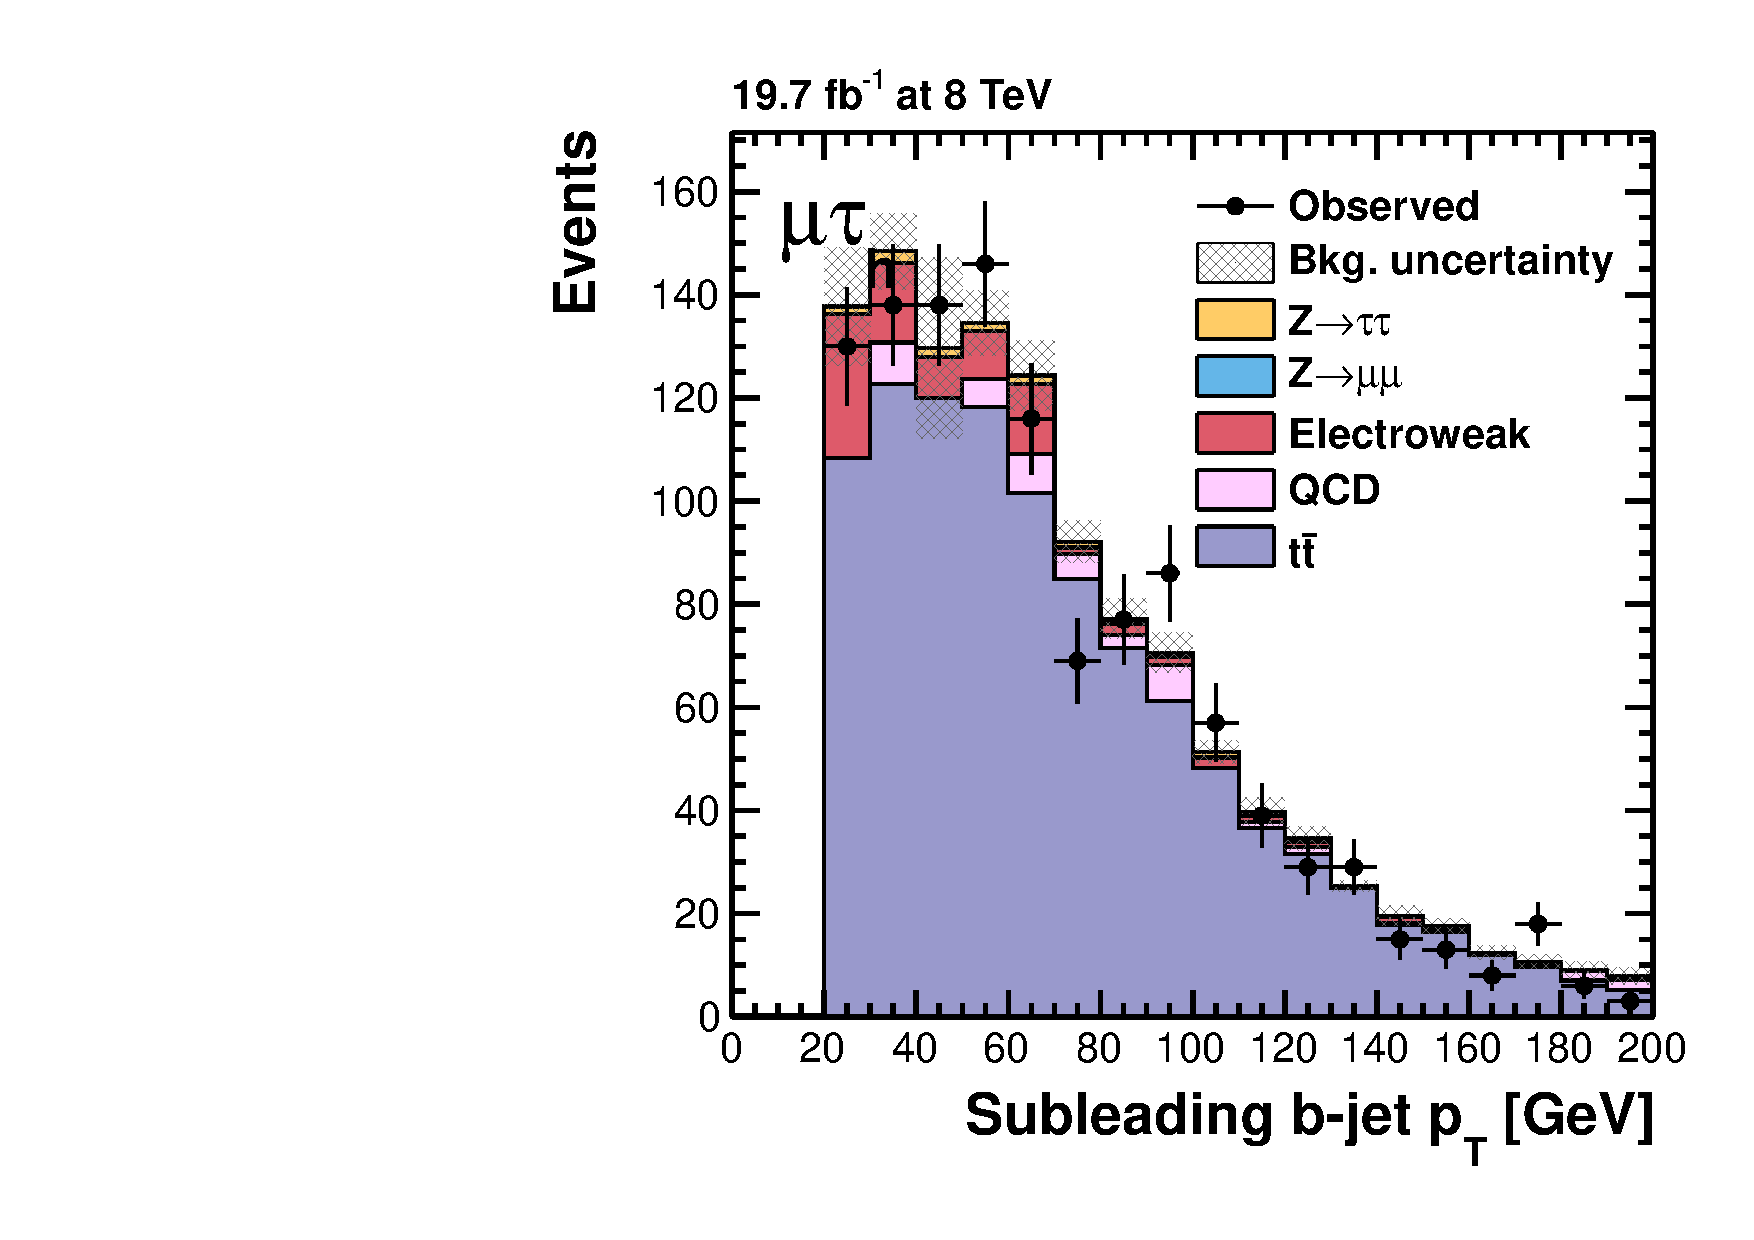
\includegraphics[width=0.5\textwidth]
      {plots/Hhh/TTBarControl/prebjetpt_2_2jet2tagSF_mt_2012.pdf}}
\end{center}
\caption[Leading and subleading b-jet $\pt$ in the $\ttbar$ control regions.]{
Leading and subleading b-jet $\pt$ in the $\ttbar$ control regions for the
$\emu$ and $\mutau$ channels as defined in the text.}
\label{fig:ttbarcontrol}
\end{figure} 

\subsection{$\WJets$}

The $\WJets$ background estimation follows that of the previous analyses, with
the normalisation in a high $m_{\text{T}}$ control region taken from data with
other backgrounds subtracted, and extrapolated to the low $m_{\text{T}}$ signal
region using a scale factor from \ac{MC}. Here,
care must be taken due to the high quantity of $\ttbar$ in the $\WJets$ control
region at high $m_{\text{T}}$ in the 2jet--1tag and 2jet--2tag categories. 
Figure~\ref{fig:2jet1tag2jet2tagmt} shows the 
$m_{\text{T}}$ distribution in the 2jet--1tag and 2jet--2tag categories for
events in the $\mutau$ channel. It can
be seen that the contribution of $\ttbar$ in the high $m_{\text{T}}$ control
regions is extremely high. If the $\ttbar$ prediction is trusted, then the data
driven subtraction method is still safe. Additional cross-checks were performed by
using events in the high $m_{\text{T}}$ region and fitting a variable in data
with good shape discrimination between $\WJets$ and $\ttbar$. Figure
\ref{fig:highmtfit} shows an example of such a fit in the 2jet--1tag category
using the discriminator of leading jet $\pt$. In the fit the contributions of
both backgrounds are allowed to float unconstrained, such that only the shapes of
the templates affect the fit. The results of such fits were generally found to be
consistent with the subtraction method within the statistical uncertainties.
The subtraction method is kept as the default method for its simplicity.  

\begin{figure}
\begin{center}
\subfloat[]{
    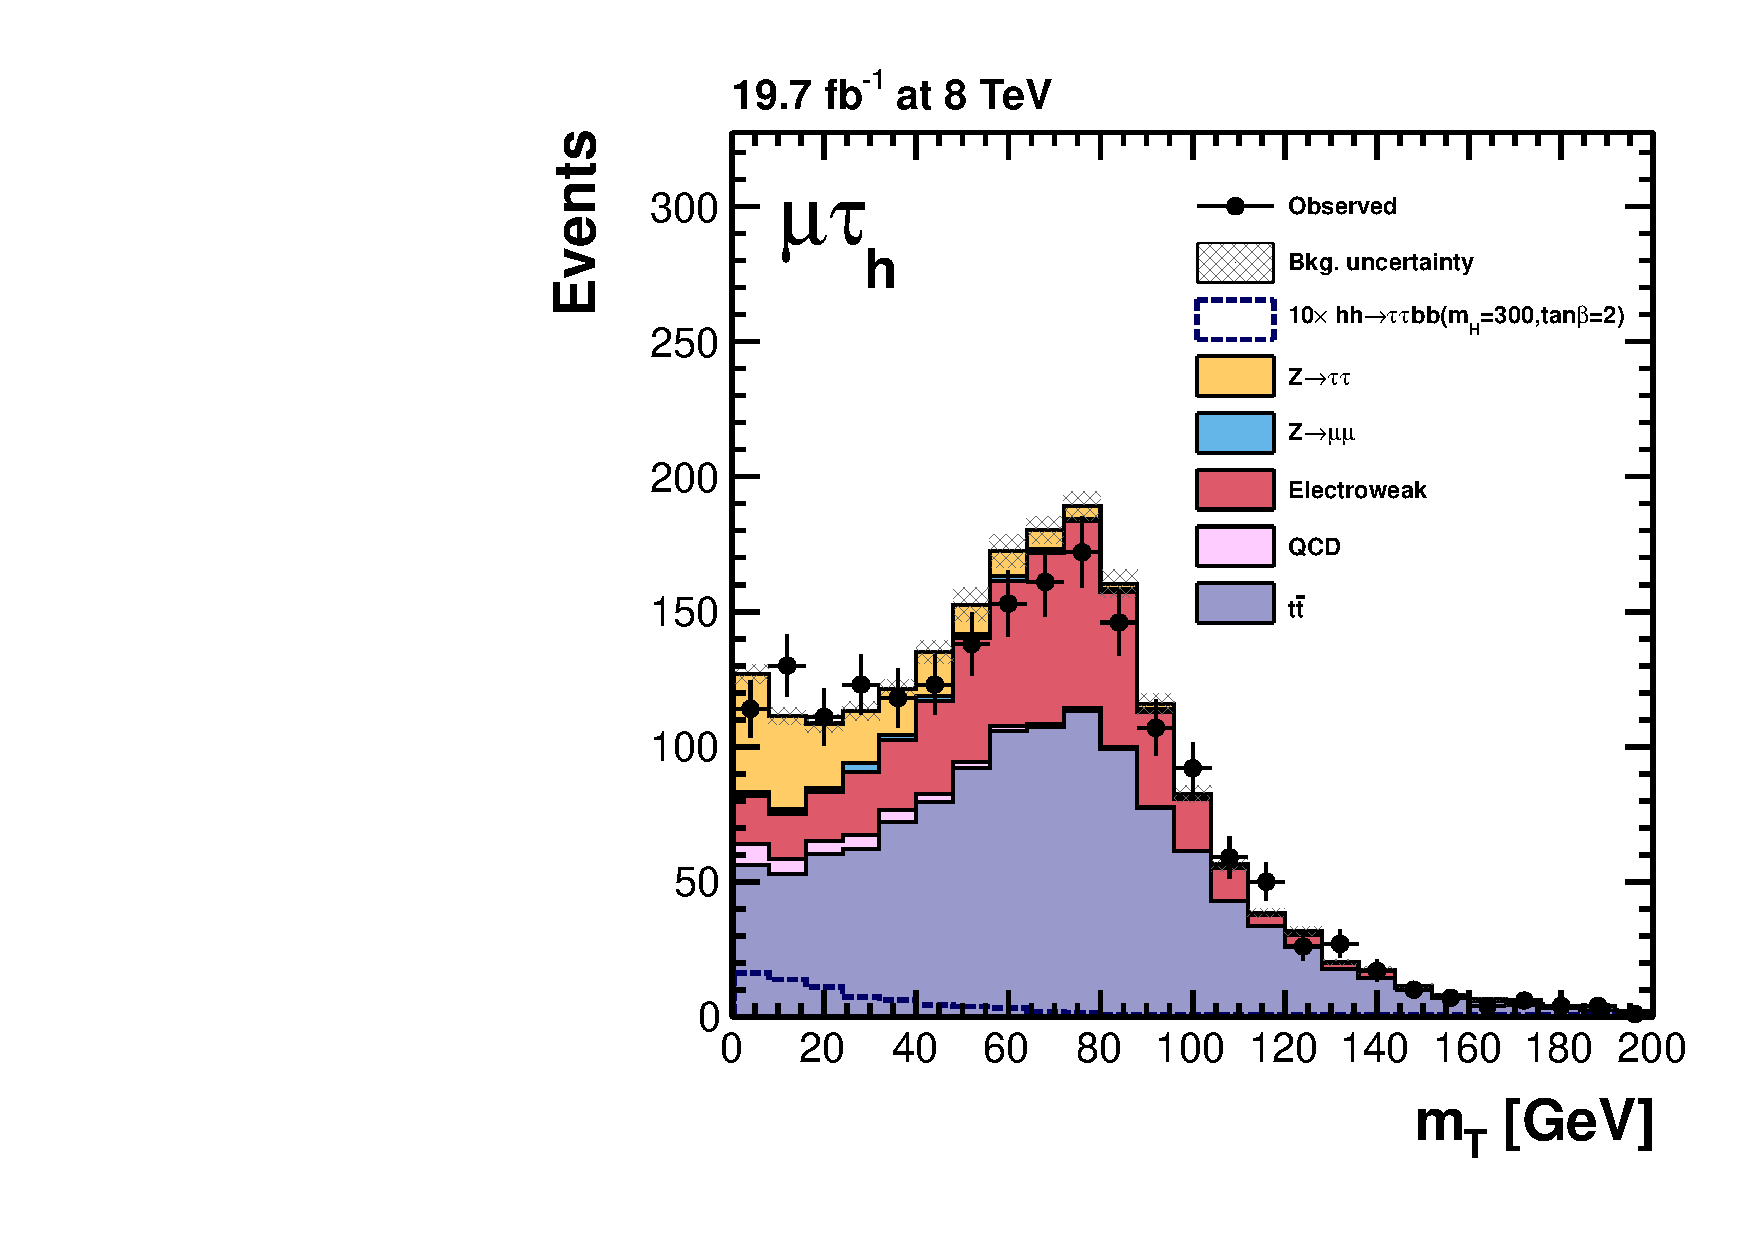
\includegraphics[width=0.5\textwidth]
      {plots/Hhh/mt_1_2jet1tagSFMassCuts_mt_2012.pdf}}
\subfloat[]{
    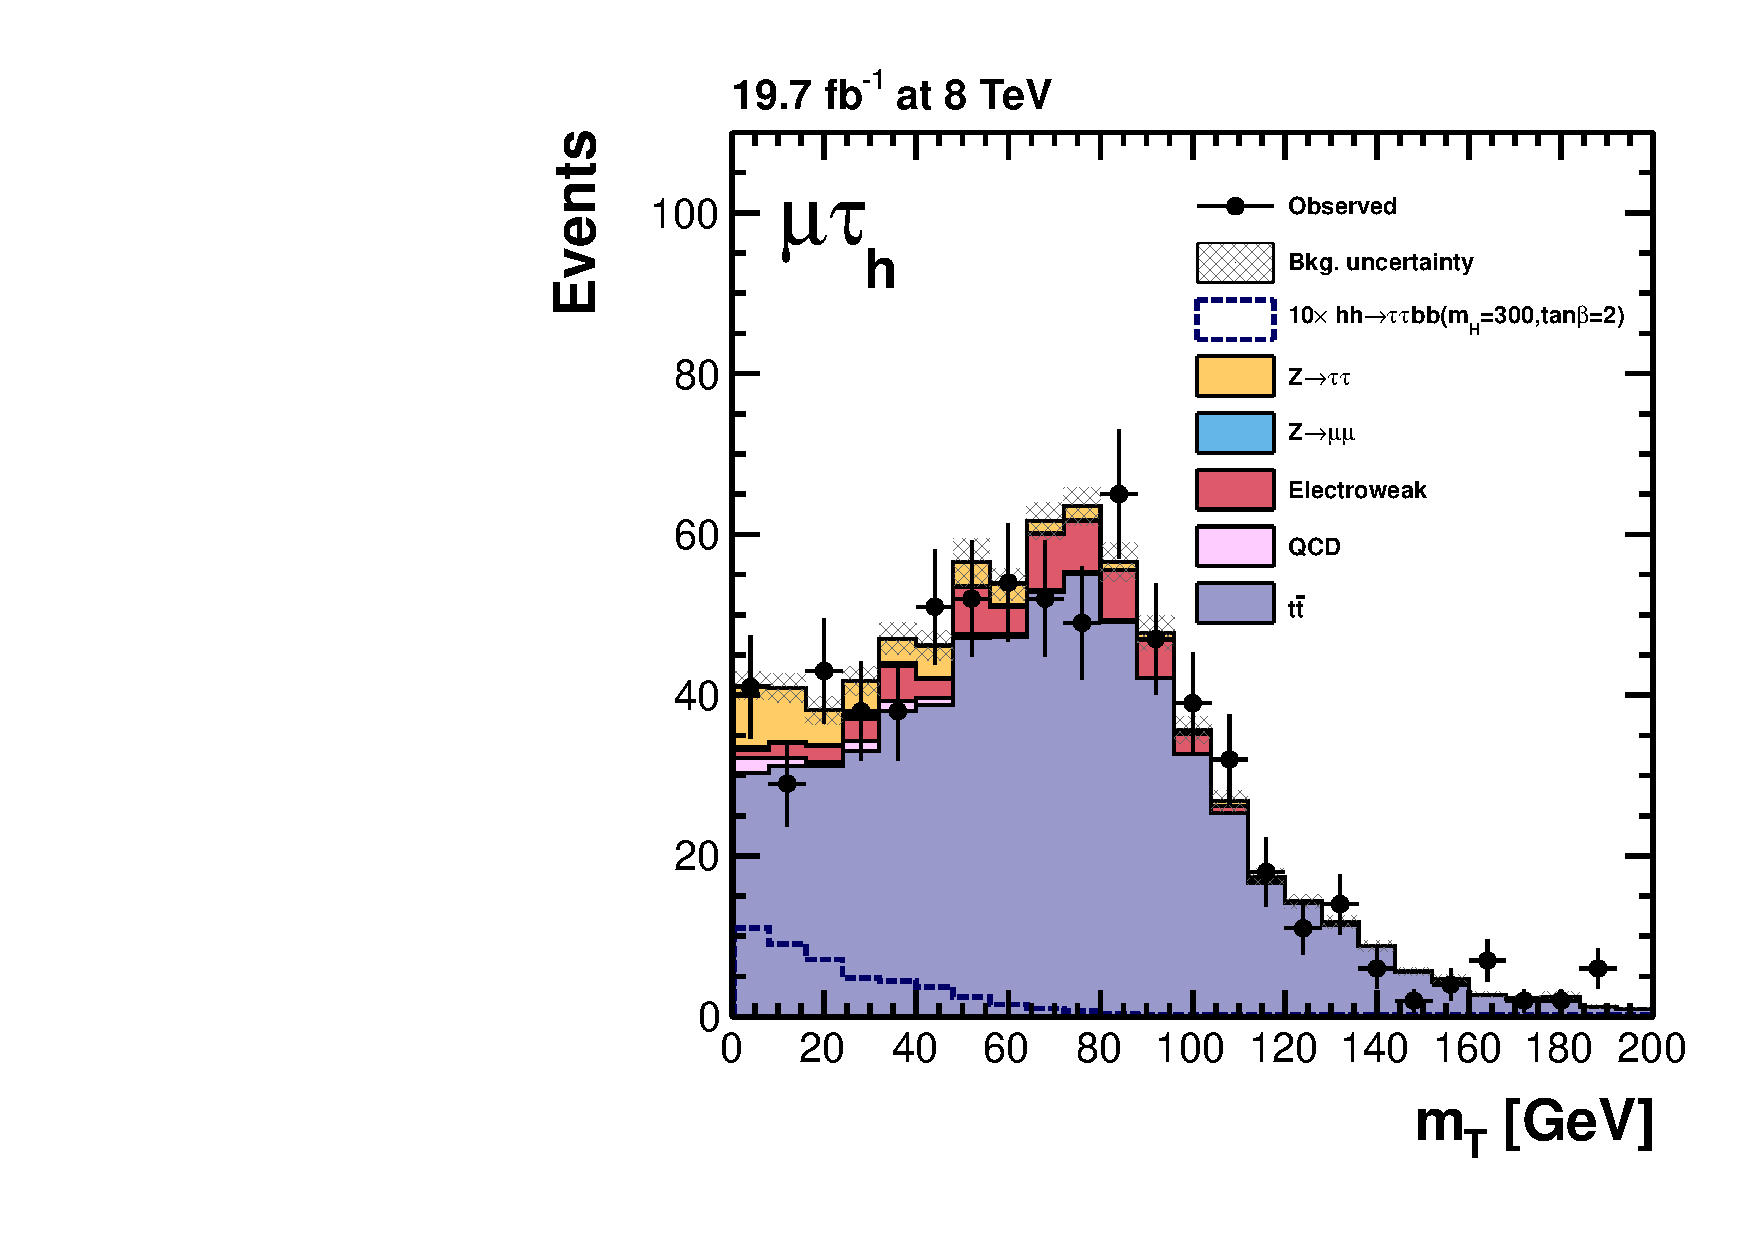
\includegraphics[width=0.5\textwidth]
      {plots/Hhh/mt_1_2jet2tagSFMassCuts_mt_2012.pdf}}

\end{center}
\caption[Transverse mass distribution for events in the 2jet--1tag (left) and
2jet--2tag (right) categories.]{
Transverse mass distribution for events in the 2jet--1tag (left) and
2jet--2tag (right) categories. The $\PW$ normalisation is taken from data in the high
$m_{\text{T}}$ region, and extrapolated to low $m_{\text{T}}$ using \ac{MC}. The
shape is also taken from \ac{MC}. In these categories, a large amount of
$\ttbar$ is present in the high $m_{\text{T}}$ region. These figures are made without any
fit to data and the uncertainty band contains only statistical uncertainty.}
\label{fig:2jet1tag2jet2tagmt}
\end{figure}


\begin{figure}
\begin{center}
    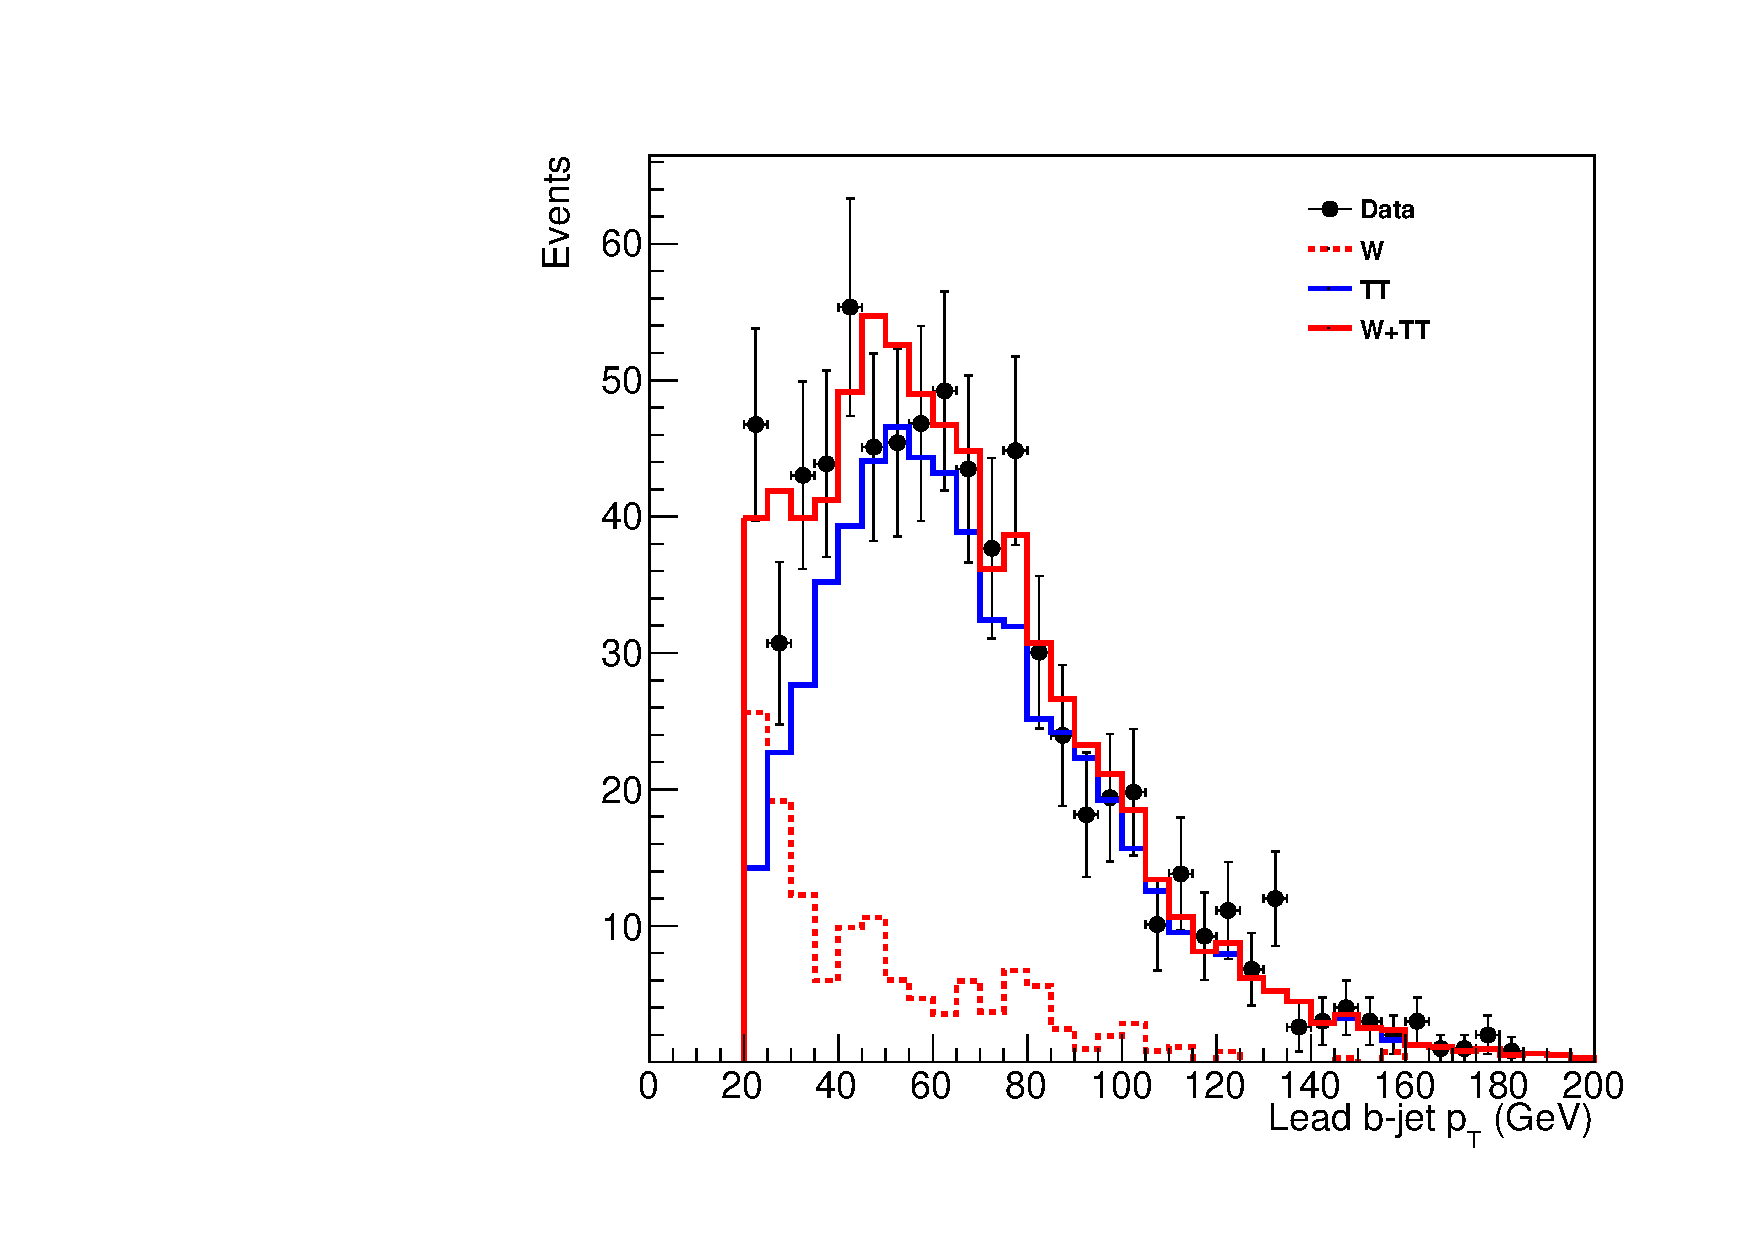
\includegraphics[width=0.5\textwidth]
      {plots/Hhh/W_TT_fit_prebjetpt_1_2jet1tag.pdf}

\end{center}
\caption[Example of a template fit for data events in the high $m_{\text{T}}$ region of the
2jet--1tag category, using the variable leading jet $\pt$.]{
Example of a template fit for data events in the high $m_{\text{T}}$ region of the
2jet--1tag category, using the variable leading jet $\pt$. The fit floats the
normalisations of the $\WJets$ and $\ttbar$ backgrounds unconstrained to best
fit the data.}
\label{fig:highmtfit}
\end{figure}

A small modification in the normalisation estimate is made to deal with the
extremely low statistics in the 2jet--2tag category. A higher purity of $\WJets$
compared with $\ttbar$ is found if the high $m_{\text{T}}$ control region is modified
slightly from $m_{\text{T}}>70~\GeV$ to $60<m_{\text{T}}<120~\GeV$.
Additionally, to avoid a huge statistical uncertainty on the extrapolation
factor estimated in \ac{MC}, the calculation is done for a relaxed category
selection using the loose \ac{CSV} working point instead of medium. 
The $\WJets$ shape is taken from the \ac{MC} estimate within the category. As
in the previous analyses, in places it is necessary to relax the category
definition to obtain a smooth shape. For both the 2jet--1tag and the 2jet--2tag
categories, this is achieved by relaxing the b-tagging condition to the
loose \ac{CSV} working point. This is found to introduce minimal bias in the
shape of the kinematic fit distribution. 

\subsection{QCD}

The QCD estimation is performed in the same data-driven way as in the previous
analyses. In the 2jet--0tag and 2jet--1tag categories, the normalisation is
taken from the same-sign data with other backgrounds subtracted. In 2jet--1tag
and 2jet--2tag, there is again a reasonable contribution from $\ttbar$ in the
data control region. The normalisation estimate is cross-checked using the anti-isolated
same-sign data, which is presumed to be entirely QCD and hence does not have the
same issues with background subtraction. The same-sign estimate for inclusive
events including at least two jets (which has a lower overall fraction of $\ttbar$
events compared with pure QCD) is extrapolated to the 2jet--1tag or 2jet--2tag
categories using an extrapolation factor calculated using the anti-isolated
data. This prediction is found to be consistent with the prediction from the
default method within the statistical uncertainties. Thus the default method is
retained for 2jet--1tag, while for 2jet--2tag the anti-isolated method is
used due to its greatly reduced statistical uncertainty. 

Shapes are taken from anti-isolated data. As used previously, in the 2jet--1tag
and 2jet--2tag categories the shape is taken from a relaxed category definition
in which the \ac{CSV} b-tag working point is relaxed to loose.

\subsection{$\PZ\to\ell\ell$, single top and diboson}

Estimates for the remaining smaller backgrounds are taken from \ac{MC}. For the
$\PZ\to\ell\ell$ component, the \ac{CSV} b-tagging condition is relaxed to the
loose working point to obtain smooth shapes in 2jet--1tag and 2jet--2tag.

\section{Systematic uncertainties}
\label{sec:Hhhsystematics}

The systematic uncertainties follow those discussed in the previous analyses,
with some small differences. 

As the \ac{CSV} values are not directly used in this analysis except to make
the choice of leading and subleading jets, it is safe to use the promote/demote
method to evaluate the b-tag scale factor uncertainties. The effect of these uncertainties 
in this analysis is illustrated in figure~\ref{fig:Hhhbtagsystematic}. The figure on the left hand
side shows \ac{MC} events which have exactly one jet with \ac{CSV} value passing the medium
working point, and so in the absence of a correction would fall into the
2jet--1tag category. It can be seen that jets are promoted or demoted such that
after the correction is applied some of the events have zero or two b-tagged
jets. Hence after the correction, only events in the central bin would fall into
the 2jet--1tag category, and the other events are reassigned to either the
2jet--0tag category (first bin) or the 2jet--2tag category (third bin). The
right hand plot shows the same effect for the events which originally have 2
b-tagged jets and would fall in the 2jet--2tag category. After the re-tagging,
some events have zero or one b-tagged jet and are reassigned to the 2jet--0tag
or 2jet--1tag categories respectively. All remaining events in the third bin and
above fall into the 2jet--2tag category. It can be seen from this plot that the
number of events being reassigned is relatively small, and the largest effect is
up to $10\%$ on $\ttbar$ events.

\begin{figure}
\begin{center}
\subfloat[]{
    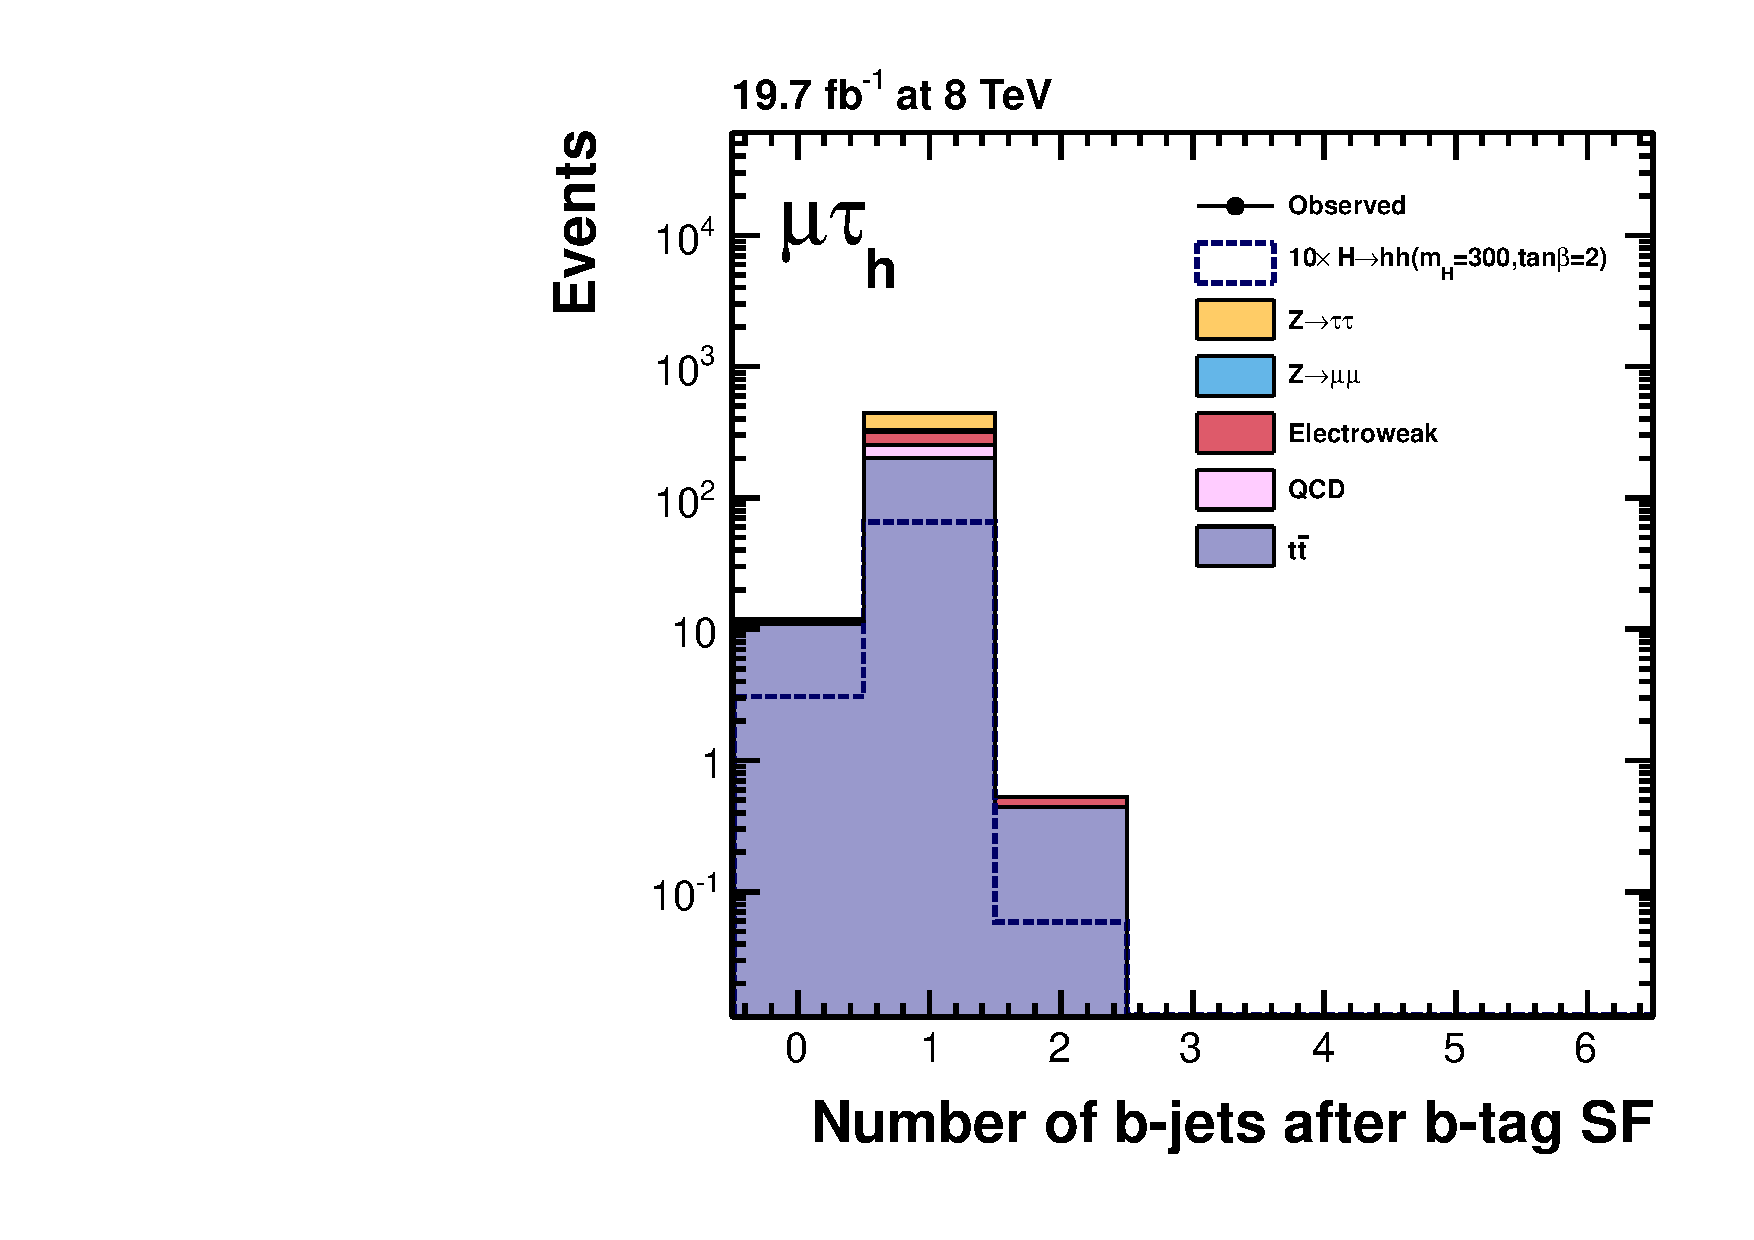
\includegraphics[width=0.5\textwidth]
      {plots/Hhh/n_prebjets_SF_2jet1tagMassCuts_mt_2012_log.pdf}}
\subfloat[]{
    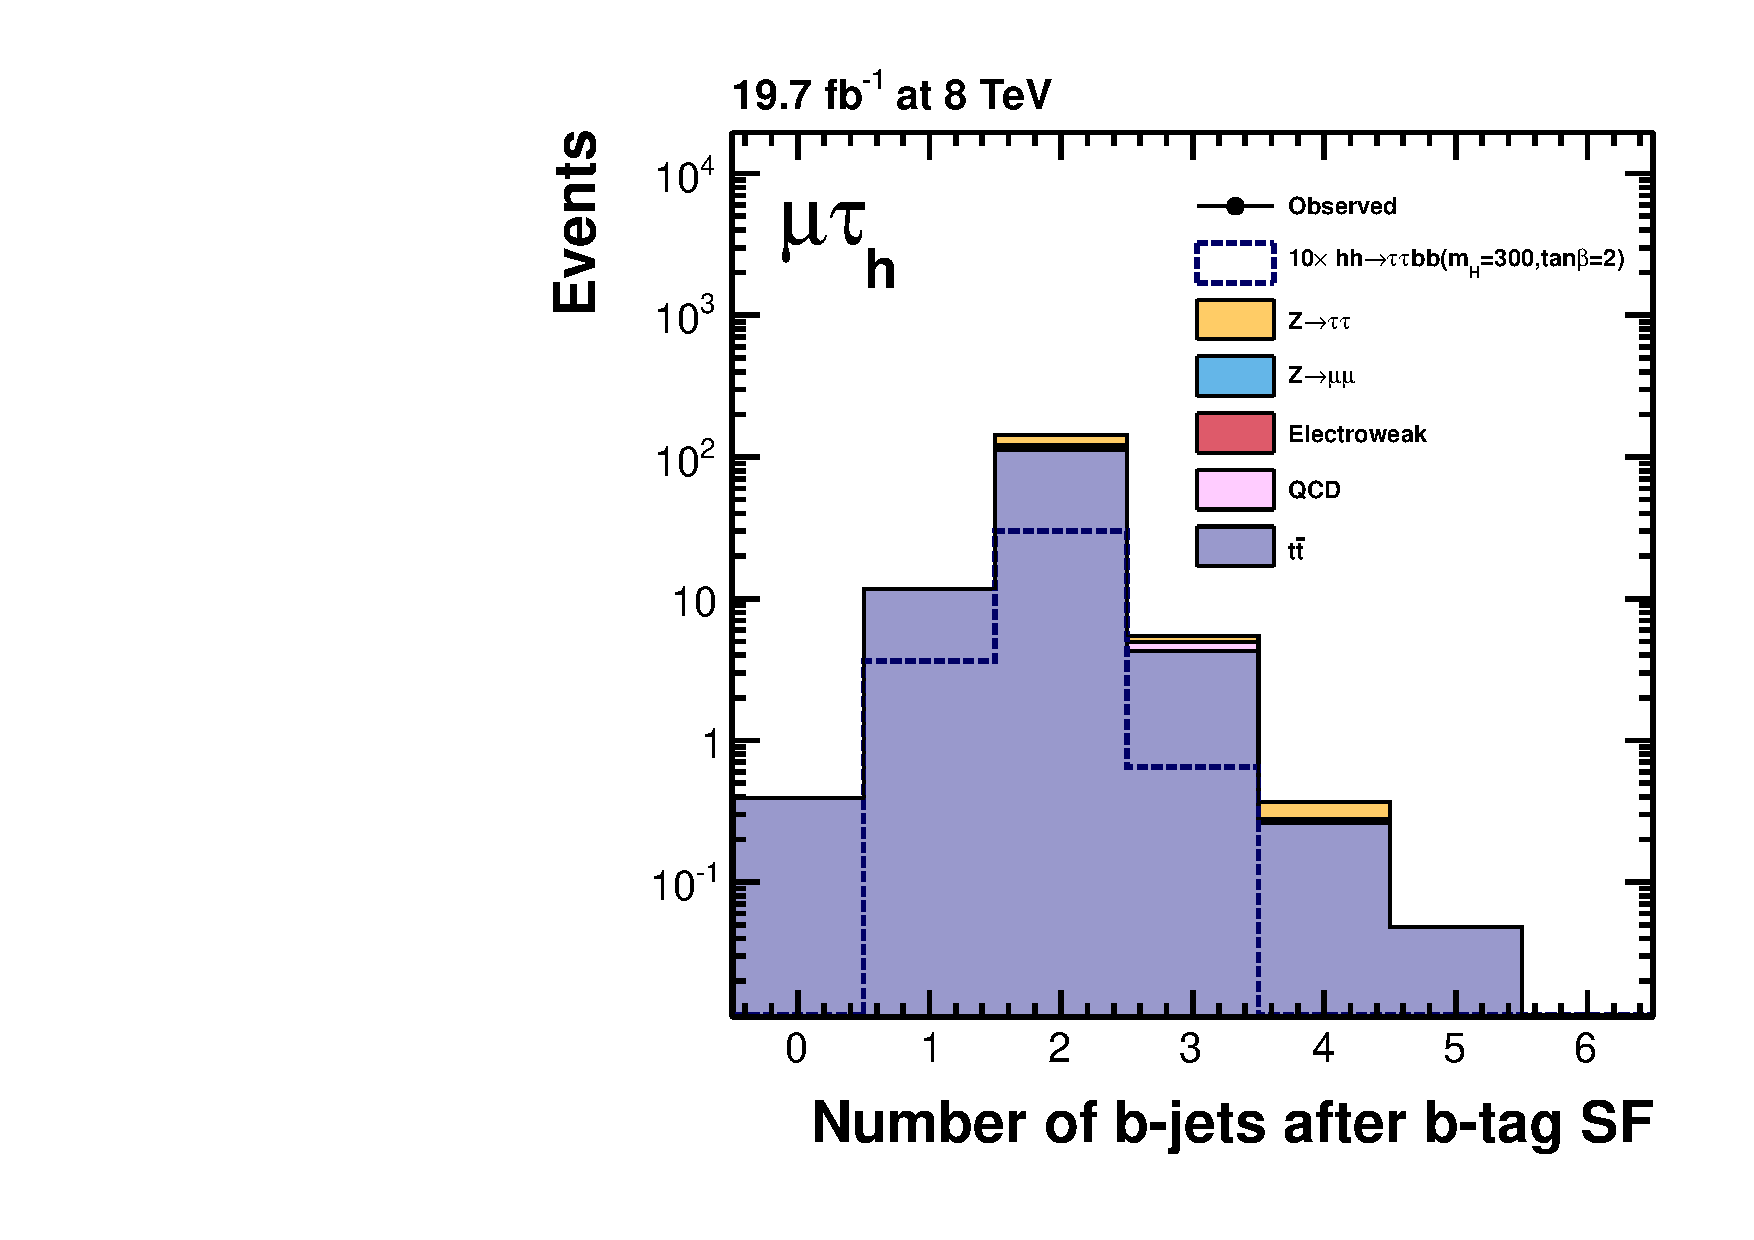
\includegraphics[width=0.5\textwidth]
      {plots/Hhh/n_prebjets_SF_2jet2tagMassCuts_mt_2012_log.pdf}}

\end{center}
\caption[Number of b-tagged jets after the b-tag scale factor is applied for events which
are originally in the 2jet--1tag (left) and 2jet--2tag (right) categories.]{
Number of b-tagged jets after the b-tag scale factor is applied for events which
are originally in the 2jet--1tag (left) and 2jet--2tag (right) categories. Jets
are promoted and demoted such that afterwards the events from one category
migrate to the other categories.}
\label{fig:Hhhbtagsystematic}
\end{figure}

The uncertainties relating to the background normalisations are re-considered
for this analysis. Some aspects, such as the $\ZToTauTau$ extrapolation factor
uncertainty, fake-rates for $\PZ\to\ell\ell$ and cross-section uncertainties on
$\ttbar$ and diboson, are the same as the previous analyses. For the
$\PZ\to\ell\ell$ background, the statistical uncertainty on the estimate is not
negligible in the 2jet--1tag and 2jet--2tag categories, and so is added in
quadrature with the uncertainty due to fake-rate. The uncertainty on the
$\PW$ and QCD estimates are dominated by limited statistics in the data control
region, and are as high as $100\%$ in 2jet--2tag. The uncertainty on the QCD
estimate includes the $10\%$ uncertainty on the opposite sign to same sign ratio
added in quadrature. For the $\PW$ estimate in 2jet--1tag, the uncertainty is
separated into two parts: one part is the propagated effect of the $10\%$
uncertainty on the $\ttbar$ control region, affecting the subtraction of
$\ttbar$ in the data control region - this is $25\%$ and is anti-correlated with
the corresponding uncertainty on the $\ttbar$ normalisation. The second part
covers the limited statistics in the data control region and is uncorrelated
with any other uncertainty, with a size of $30\%$.

An additional uncertainty on the $\ZToTauTau$ estimate, corresponding to the
size of the subtraction of the $\ttbar$ contamination in the embedded, is
included. 

Since the discriminating variable in this analysis is computed using the taus
and the jets, both the tau and jet energy scales must be applied as a shape
uncertainty. The size of the jet energy scale uncertainty is computed exactly as
in section \ref{sec:systematicUncertainties_yield}, but the change in the shape
as a result of the shift up and down in energy scale is retained as well as 
computing the change in normalisation. The effect of the jet energy scale
on the shape of the distributions for the $\ttbar$ background and the signal is
shown in figure~\ref{fig:kinfitjes}.

\begin{figure}
\begin{center}
\subfloat[]{
    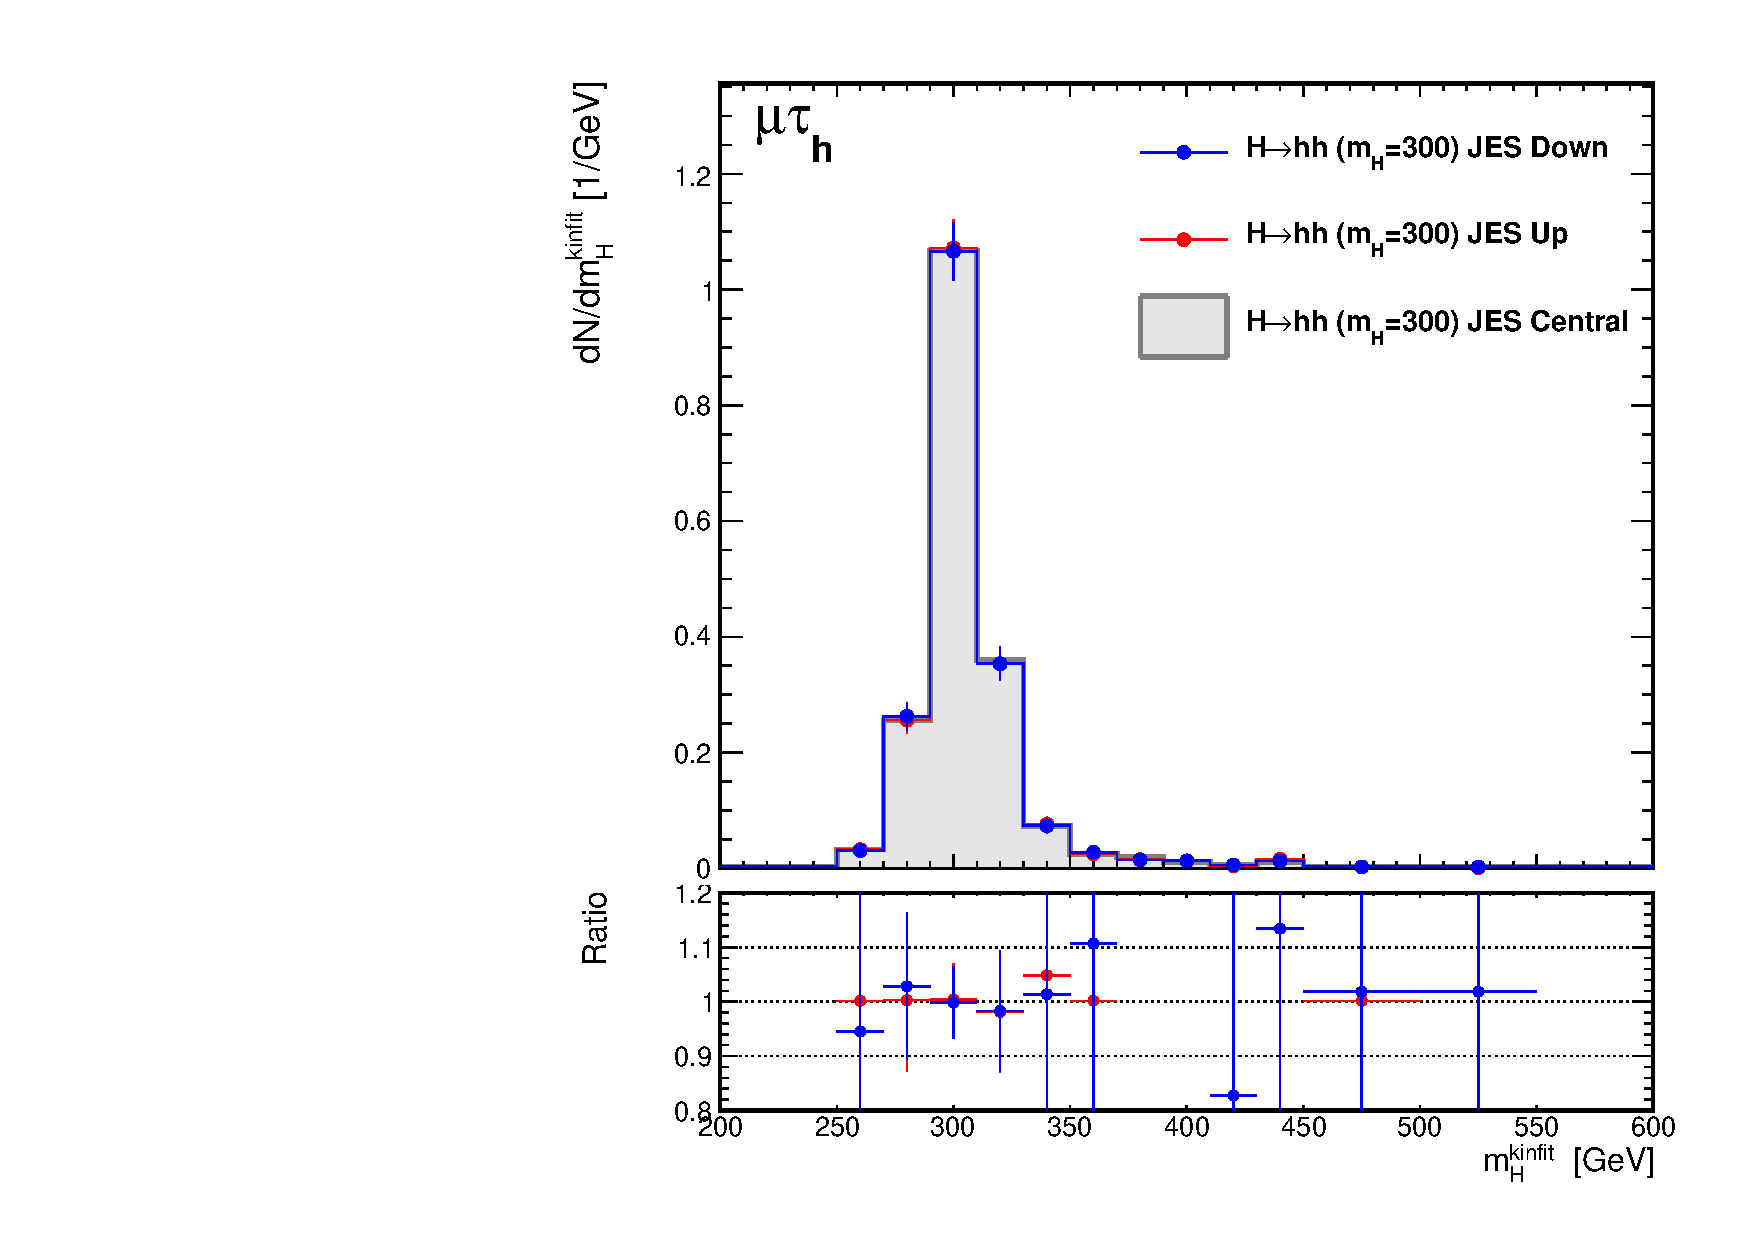
\includegraphics[width=0.5\textwidth]
      {plots/Hhh/ggHTohh300_jes_2jet2tag_mt.pdf}}
\subfloat[]{
    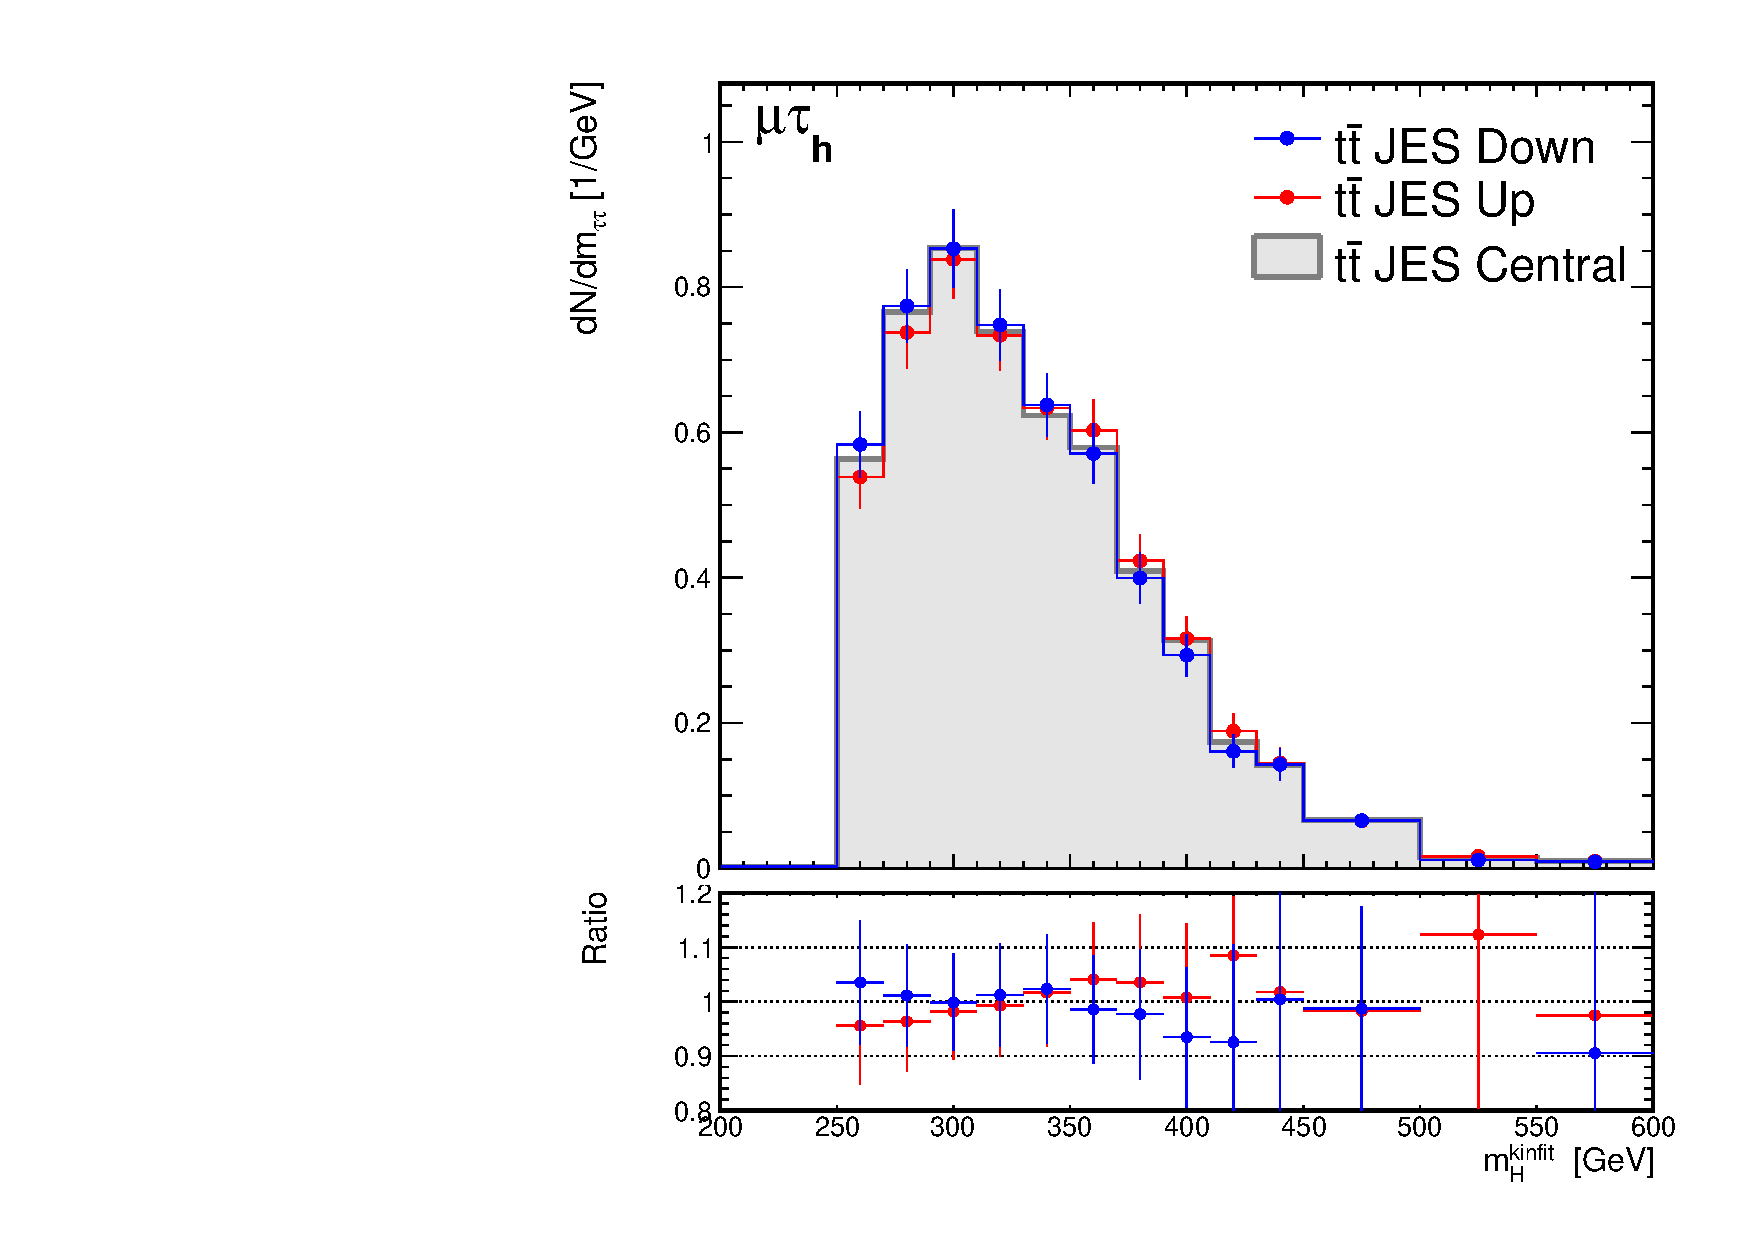
\includegraphics[width=0.5\textwidth]
      {plots/Hhh/TT_jes_2jet2tag_mt.pdf}}

\end{center}
\caption[Effect of the jet energy scale uncertainty on the kinematic fit distribution for
the signal with $m_{\PH}=300\,\GeV$ (left) and the $\ttbar$ background (right).]{
Effect of the jet energy scale (JES) uncertainty on the kinematic fit distribution for
the signal with $m_{\PH}=300\,\GeV$ (left) and the $\ttbar$ background (right).
The shift up or down in the JES can cause both the shape and normalisation to
vary, but only the effect on the shape is shown here. 
The signal is normalised to a cross-section of $1\,\picobarn$ in this figure.}
\label{fig:kinfitjes}
\end{figure} 

The treatment for templates with bins with large statistical uncertainties
follows the bin-by-bin approach used in the \ac{SM} analysis and described in
section \ref{sec:systematicUncertainties_shape}. 

The full set of systematic
uncertainties and their chosen sizes for each channel and category is given in
table \ref{tab:HhhSystematics}.


\begin{table}[tbhp]
\begin{center}
    \begin{tabular}{|l|c|c|c|c|}
    \hline
    \multicolumn{2}{|c|}{Source of uncertainty and affected signal/backgrounds} & \multicolumn{3}{|c|}{Event yield uncertainty}  \\
    \multicolumn{2}{|c|}{} & \multicolumn{3}{|c|}{by event category} \\
    \hline
     Experimental uncertainty                                  & Affected processes &  2jet--0tag    &  2jet--1tag  &  2jet--2tag      \\
     \hline
     Integrated luminosity $8\,\TeV$                           & All MC & 2.6\% & 2.6\% & 2.6\%       \\
     Electron ID and trigger                                   & All MC &  2\%  & 2\%  & 2\%       \\
     Muon ID and trigger                                       & All MC & 2--3\%       &   2--3\%    & 2--3\%       \\
     Tau ID and trigger                                        & All MC & 8\%  & 8\% & 8\%           \\
     b-tagging efficiency                                      & All MC & 1--8\% &   1--5\%  & 1--70$^{1}$\% \\
     b-mistag rate                                             & All MC & 1\%    &   1--4\%  &   1--5\%       \\
     \hline
     $\PZ$ production                                          & $\ZToTauTau$, $\PZ\to\ell\ell$ & 3.3\%     &   3.3\%    & 3.3\%      \\
     $\PZ\to\Pgt\Pgt$: category selection                      & $\ZToTauTau$ & 5\%  & 5\% & 6\%        \\
     $\PZ\to\Pgt\Pgt$: $\ttbar$ contamination                  & $\ZToTauTau$ & \%  & \% & \%        \\
     Norm. $\ttbar$                                            & $\ttbar$, $\WJets$ in 2jet--1tag & 10\%  &   10-25\%  &  10\%        \\
     Norm. di-boson                                            & diboson & 15\%   &   15\%  &  15\%      \\
     Norm. QCD                                                 & QCD  & 10\%    &   40\% & 60-100\%         \\
     Norm. $\WJets$                                            & $\WJets$ & 10\% &  40\% & 100\%             \\
     $\Pe$ misidentified as $\Pgth$                            & $\PZ\to\Pe\Pe$ & 20\%     & 20\%   & 40\%      \\
     $\Pgm$ misidentified as $\Pgth$                           & $\PZ\to\Pmu\Pmu$ & 30\%     & 60\% & 60\%         \\
     Jet misidentified as $\Pgth$                              & $\PZ+$jets & 20\%    & 20-25\% & 70-90\%             \\
     \hline
     Tau energy scale                                          & All MC & shape & shape & shape \\
     Jet energy scale                                          & All MC & shape  &   shape  & shape       \\
     \MET scale                                                & All MC & 1--7\% &   1--5\%    & 1--10\%      \\
     \hline
     \end{tabular}
    \caption[Systematic uncertainties that affect the estimated number of signal or
    background events in the $\Hhh$ analysis.]{
    Systematic uncertainties that affect the estimated number of signal or
    background events. Several uncertainties are treated as correlated for the
    different decay channels and event categories. Some uncertainties vary
    across final states and for different affected processes, so ranges are given.}
     \label{tab:HhhSystematics}
     \end{center}
     \vspace{0.5cm}
     {\justifying{ \footnotesize $^{1}$ This large uncertainty only applies to the $\WJets$
     background, which is affected by the b-tag efficiency due to the large
     contamination of $\ttbar$ in the $\WJets$ control region. The statistical
     uncertainty on $\WJets$ in 2jet--2tag is overwhelmingly larger than any
     systematic component.}\par 
     }
\end{table}


\section{Results}
\label{sec:Hhhresults}

\subsection{Signal Extraction}

The 4-body mass after kinematic fit is used as the discriminating variable for
signal extraction. A maximum likelihood fit is performed in all channels and
categories simultaneously following exactly the methods described in section
\ref{sec:signalextraction}. The final kinematic fit distributions are shown in
figures~\ref{fig:PostFitMHmutau} and \ref{fig:PostFitMHetau}.

\begin{figure}
\begin{center}
\subfloat[]{
    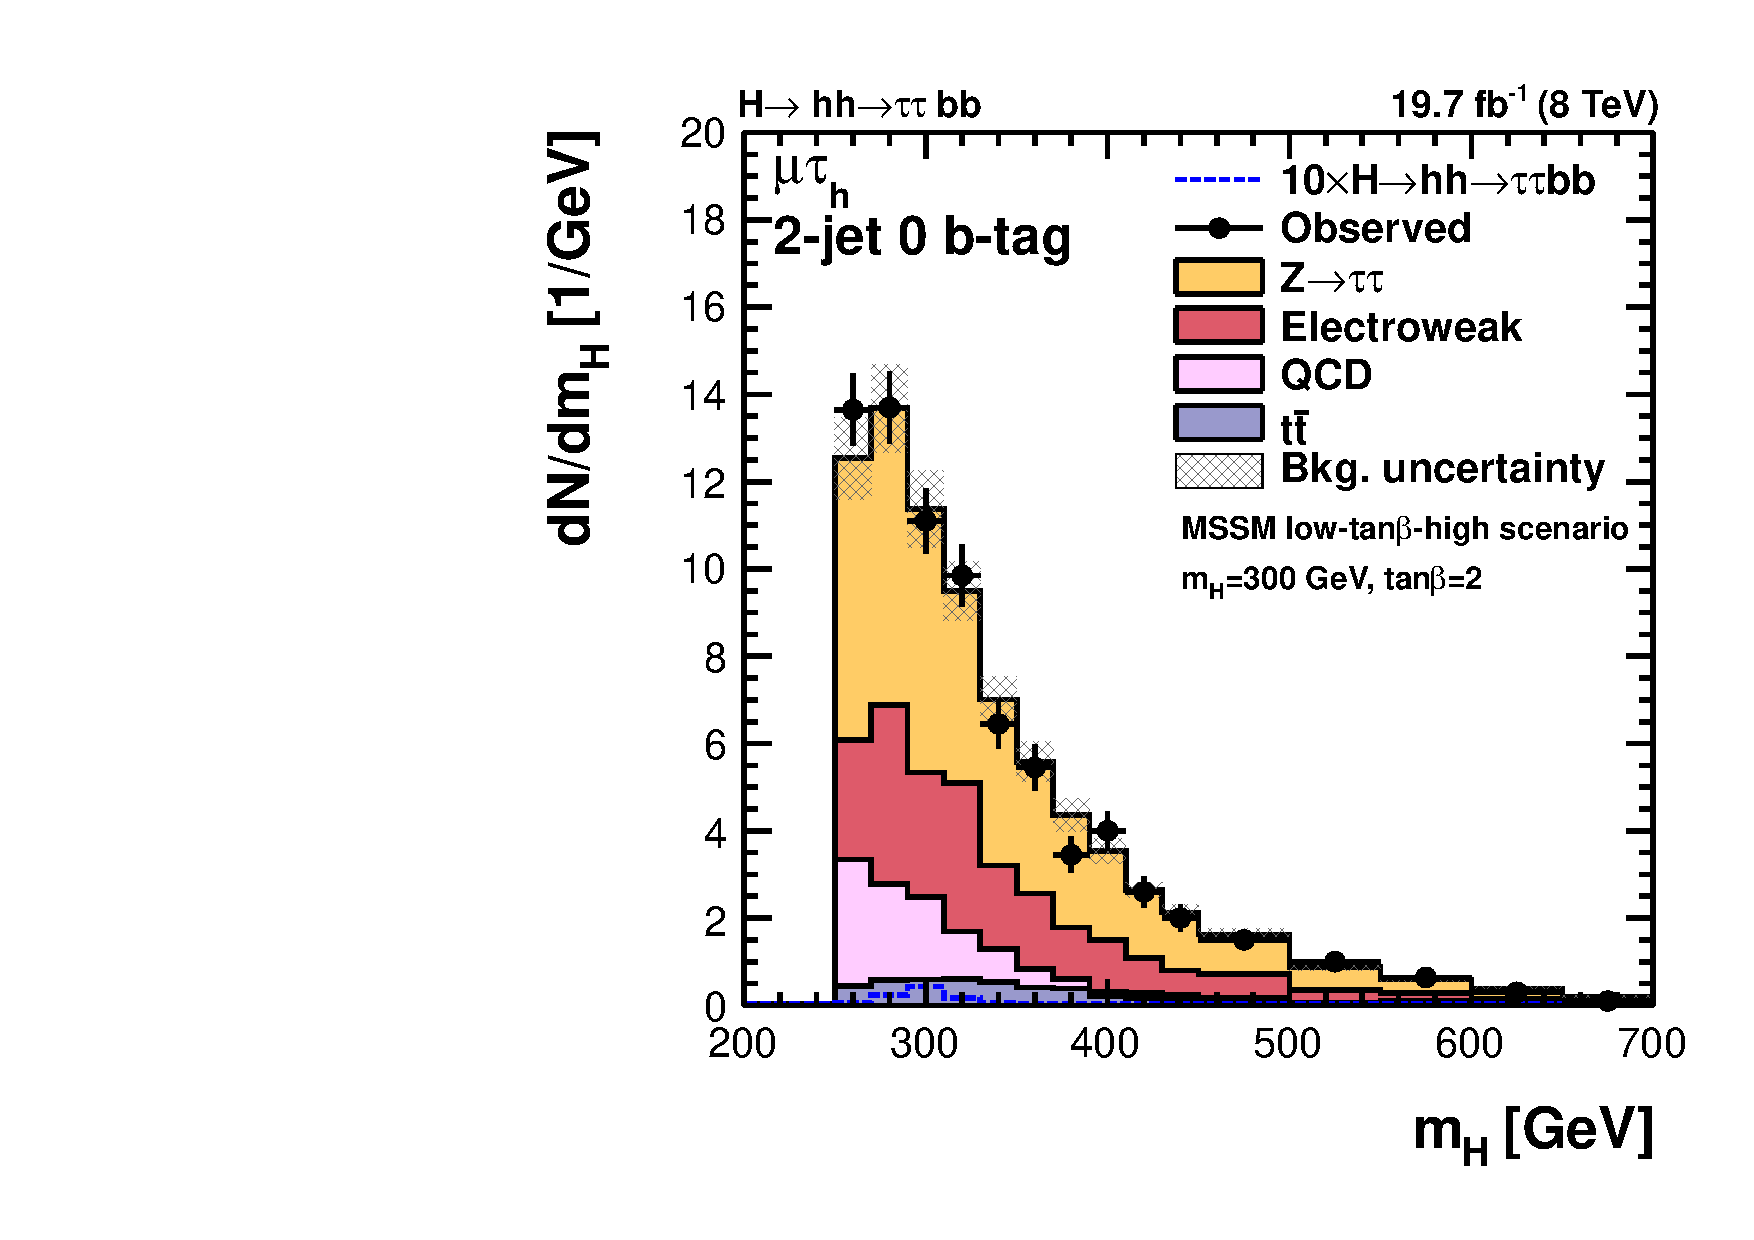
\includegraphics[width=0.5\textwidth]
      {plots/Hhh/muTau_2jet0tag_postfit_8TeV_LIN.pdf}}
\subfloat[]{
    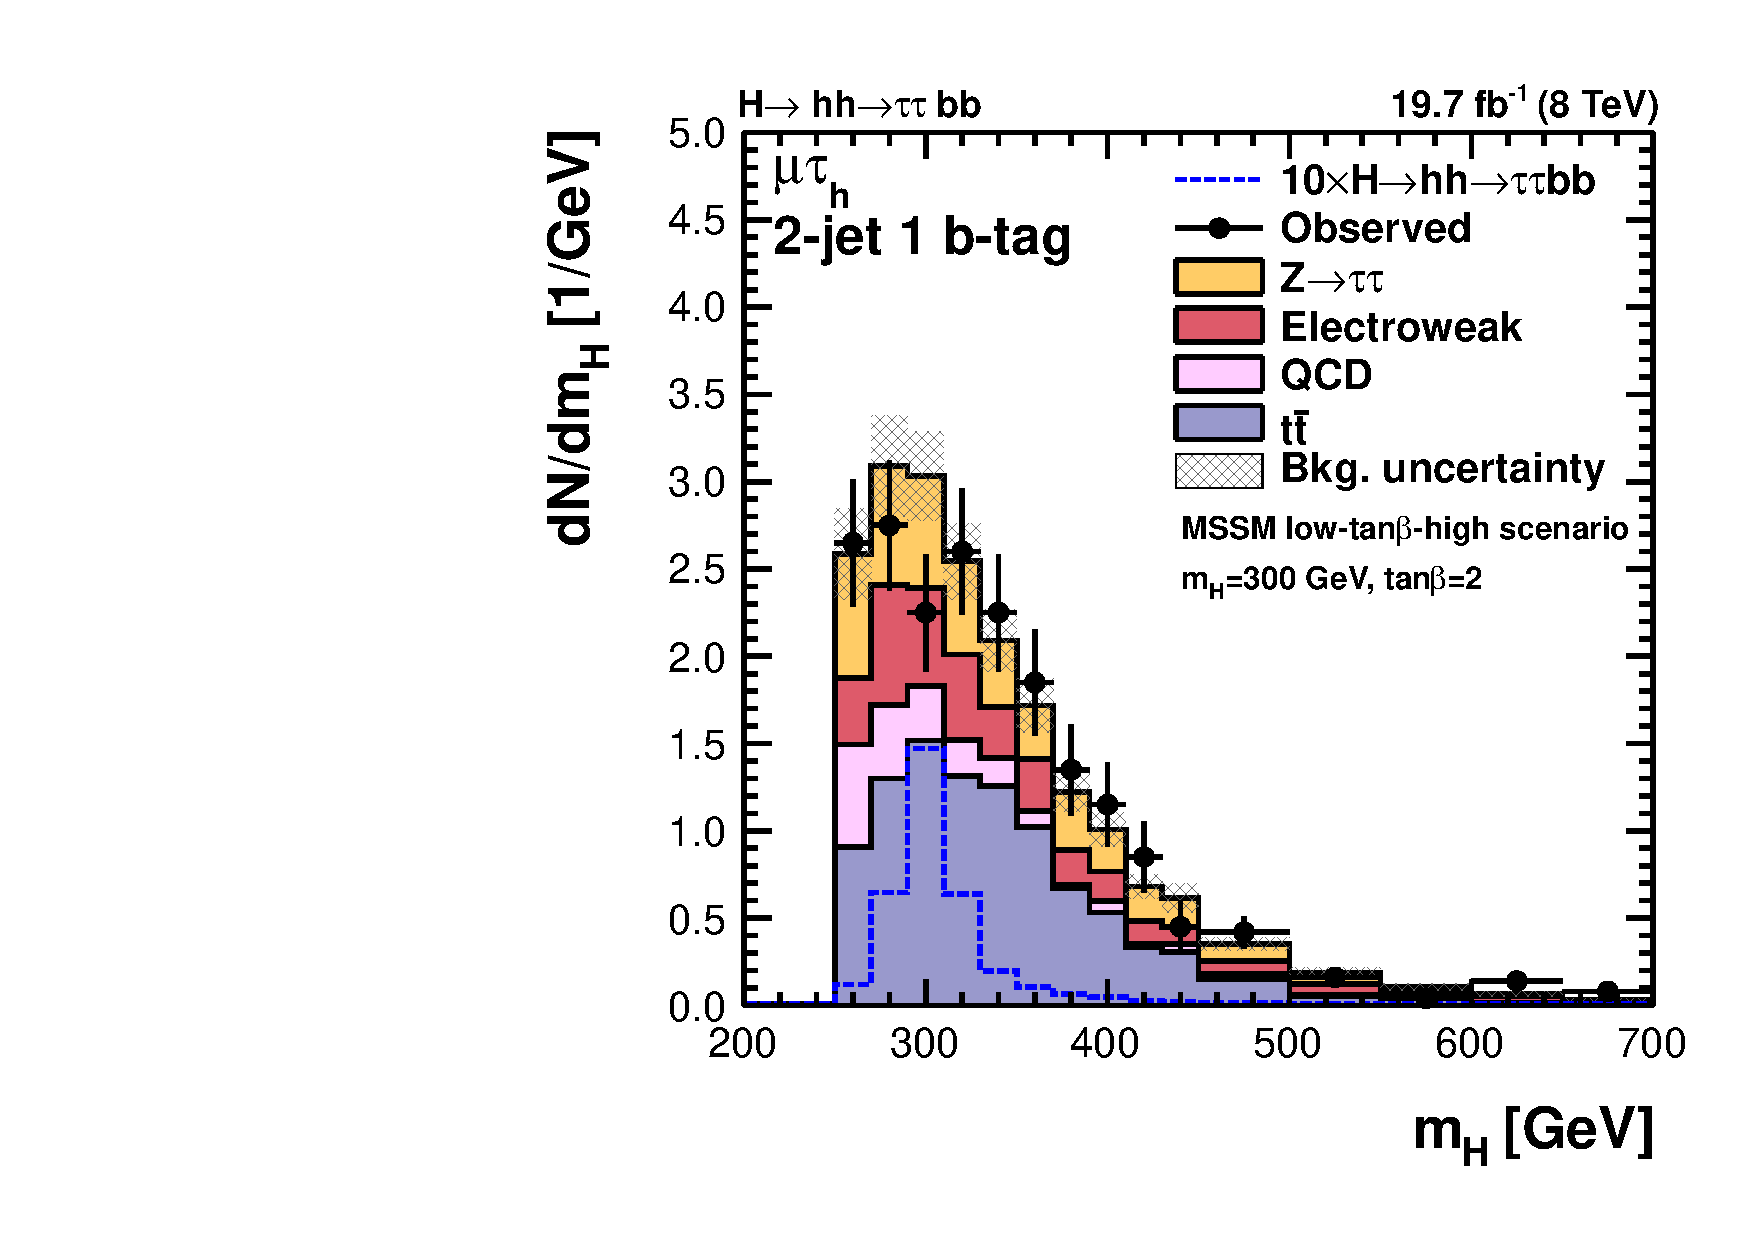
\includegraphics[width=0.5\textwidth]
      {plots/Hhh/muTau_2jet1tag_postfit_8TeV_LIN.pdf}}

\subfloat[]{
    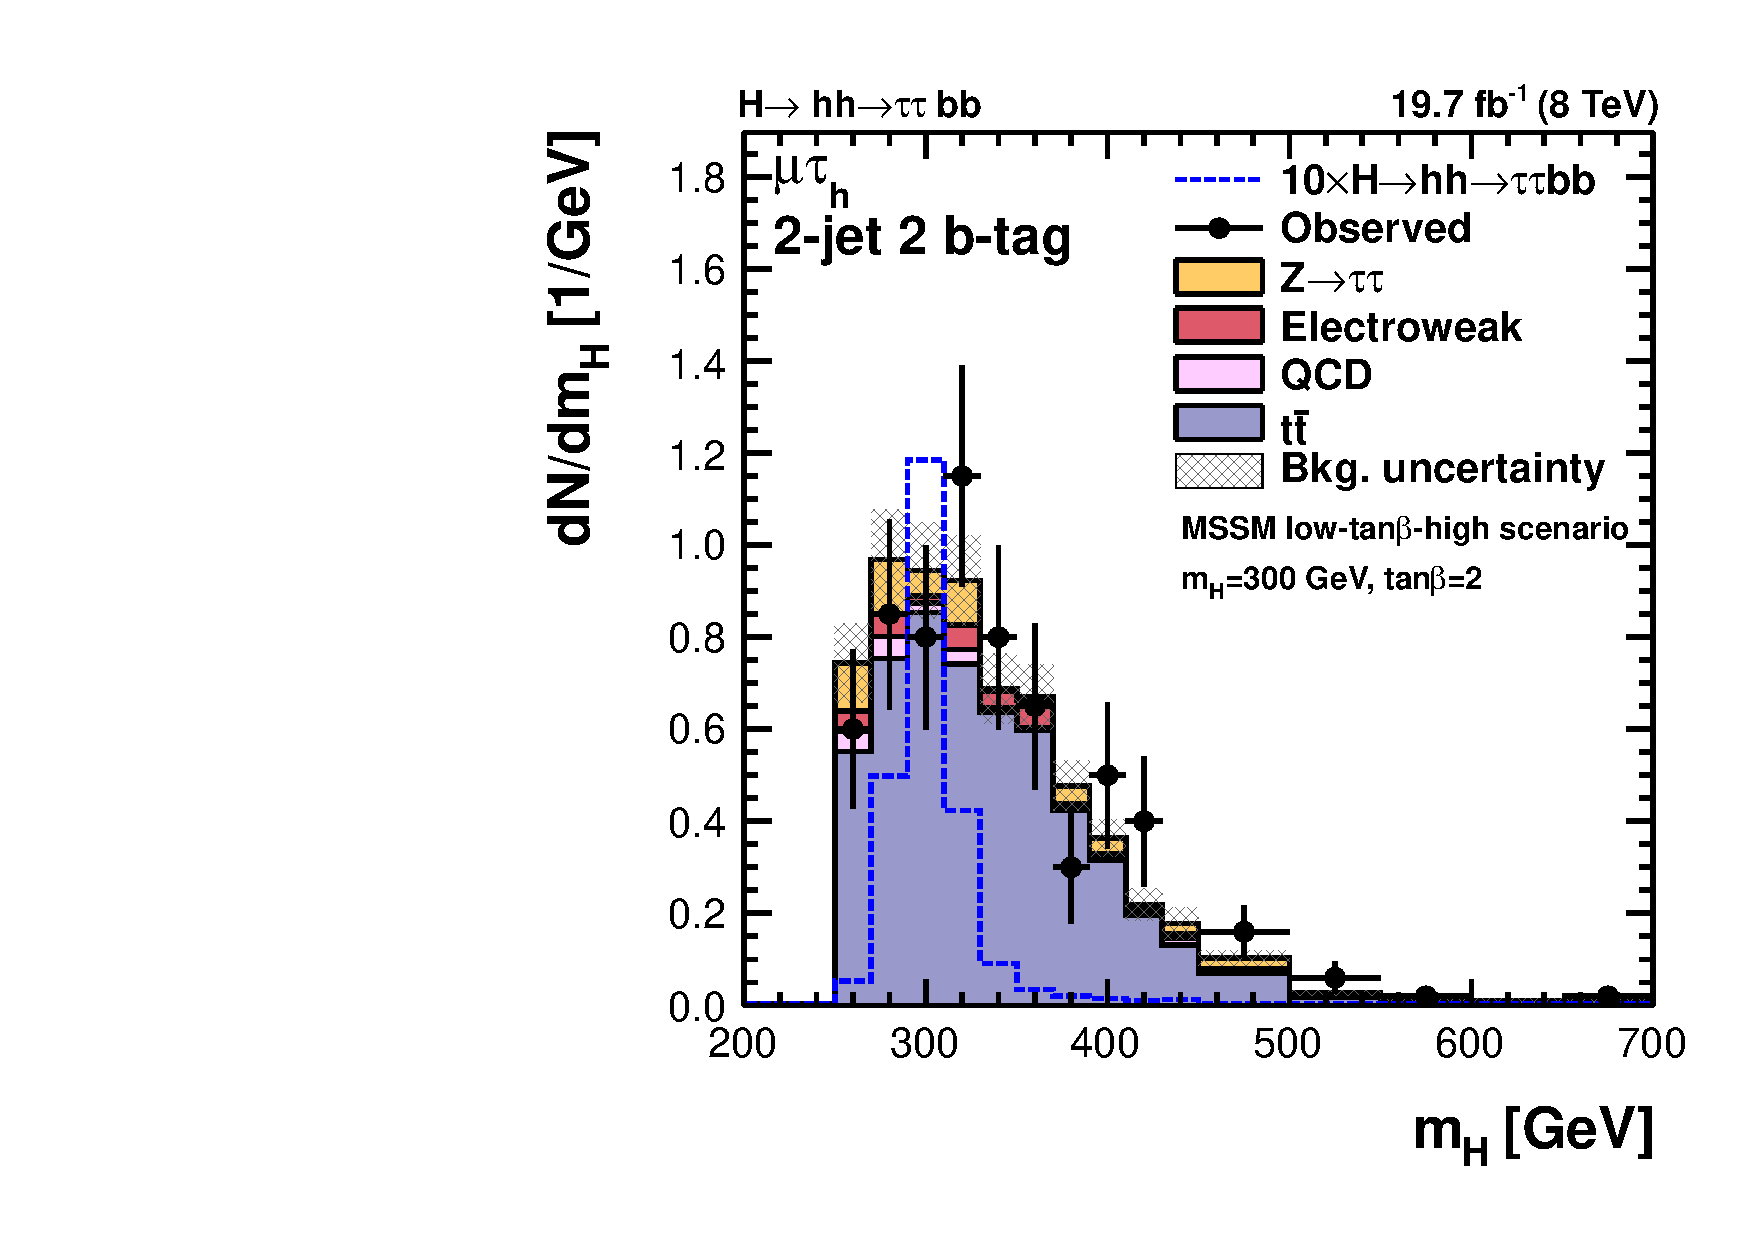
\includegraphics[width=0.5\textwidth]
      {plots/Hhh/muTau_2jet2tag_postfit_8TeV_LIN.pdf}}
\end{center}
\caption{
Distributions of kinematic fit mass following the maximum likelihood fit for
events in the $\mutau$ channel and the 2jet--0tag (top left) 2jet--1tag (top
right) and 2jet--2tag (bottom) categories. Signal is shown for a benchmark
cross-section times branching ratio for $m_{\PH}=300\,\GeV$ and $\tan\beta=2$
and scaled by a factor of 10 to make it visible.}
\label{fig:PostFitMHmutau}
\end{figure} 


\begin{figure}
\begin{center}
\subfloat[]{
    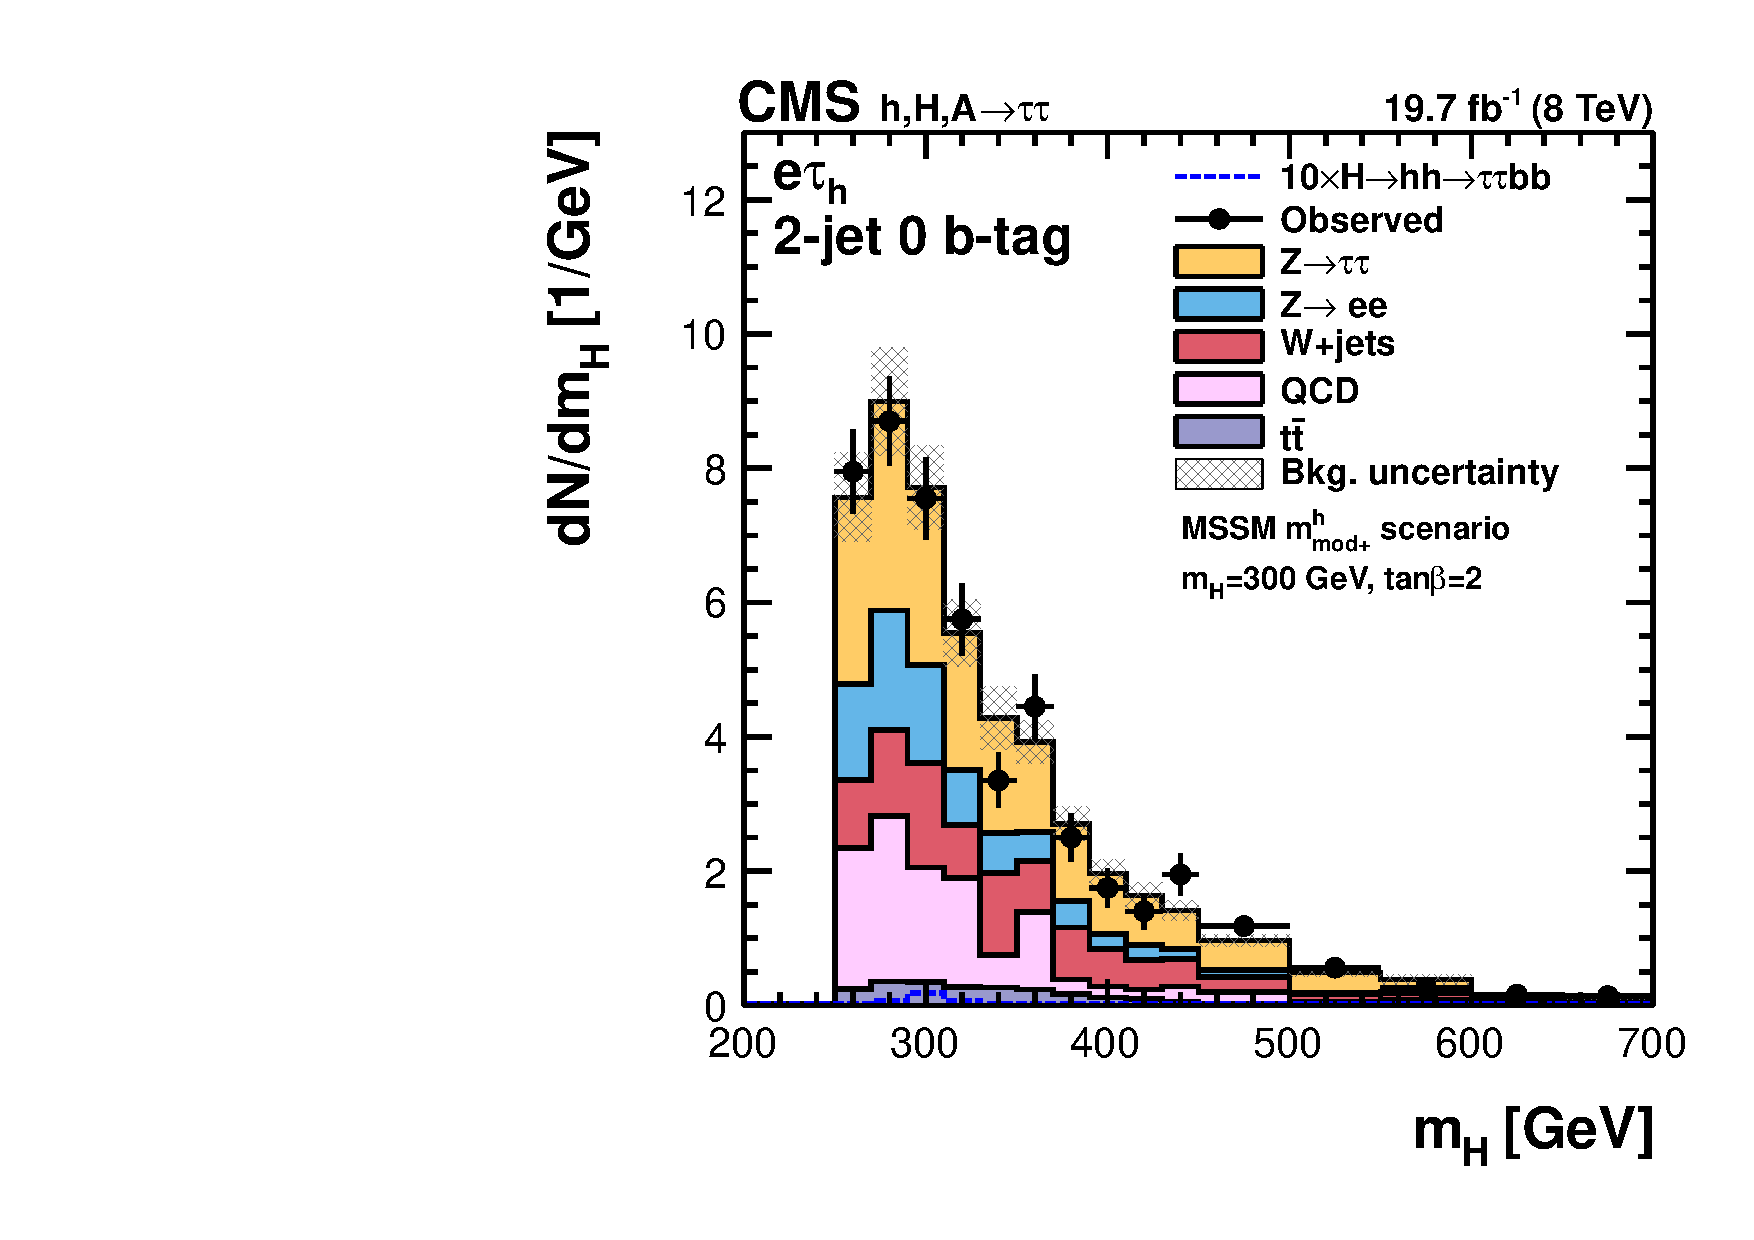
\includegraphics[width=0.5\textwidth]
      {plots/Hhh/eleTau_2jet0tag_postfit_8TeV_LIN.pdf}}
\subfloat[]{
    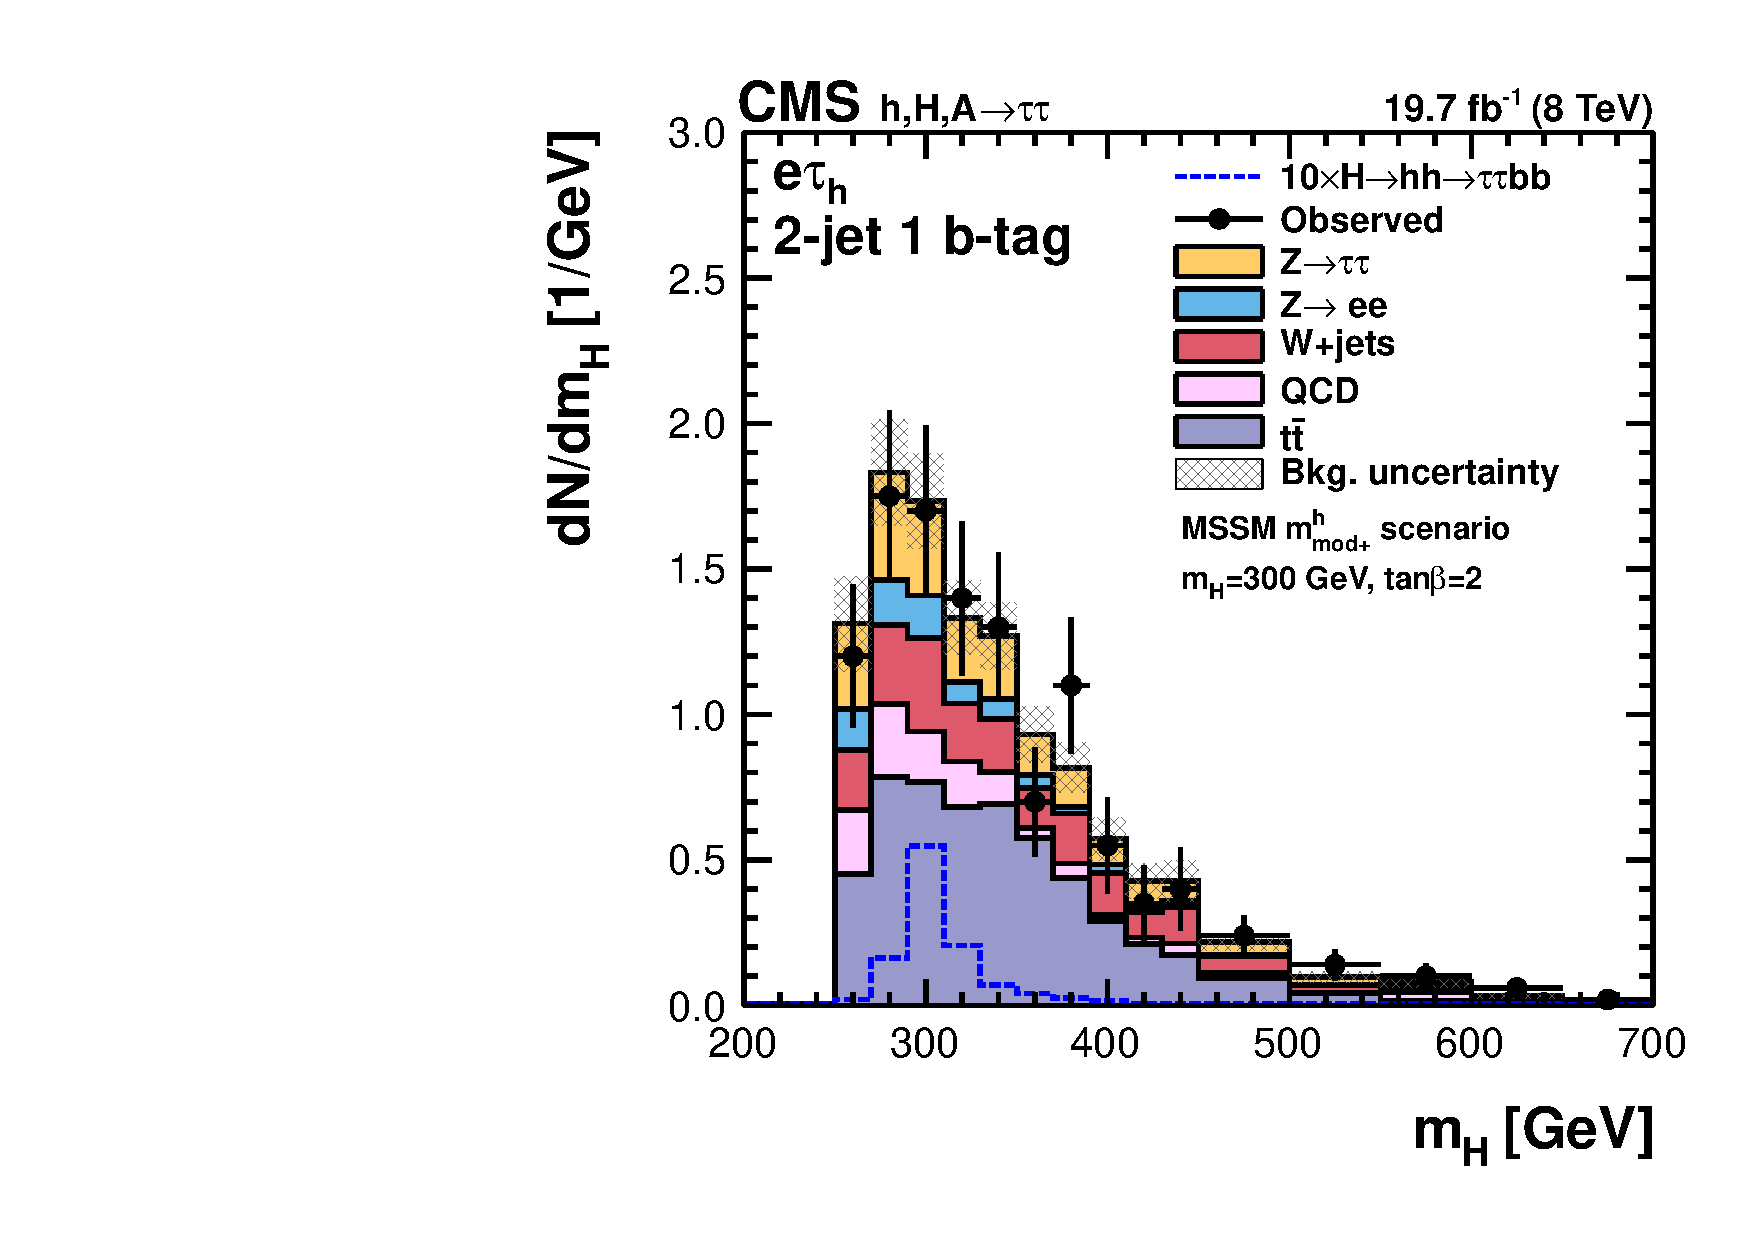
\includegraphics[width=0.5\textwidth]
      {plots/Hhh/eleTau_2jet1tag_postfit_8TeV_LIN.pdf}}

\subfloat[]{
    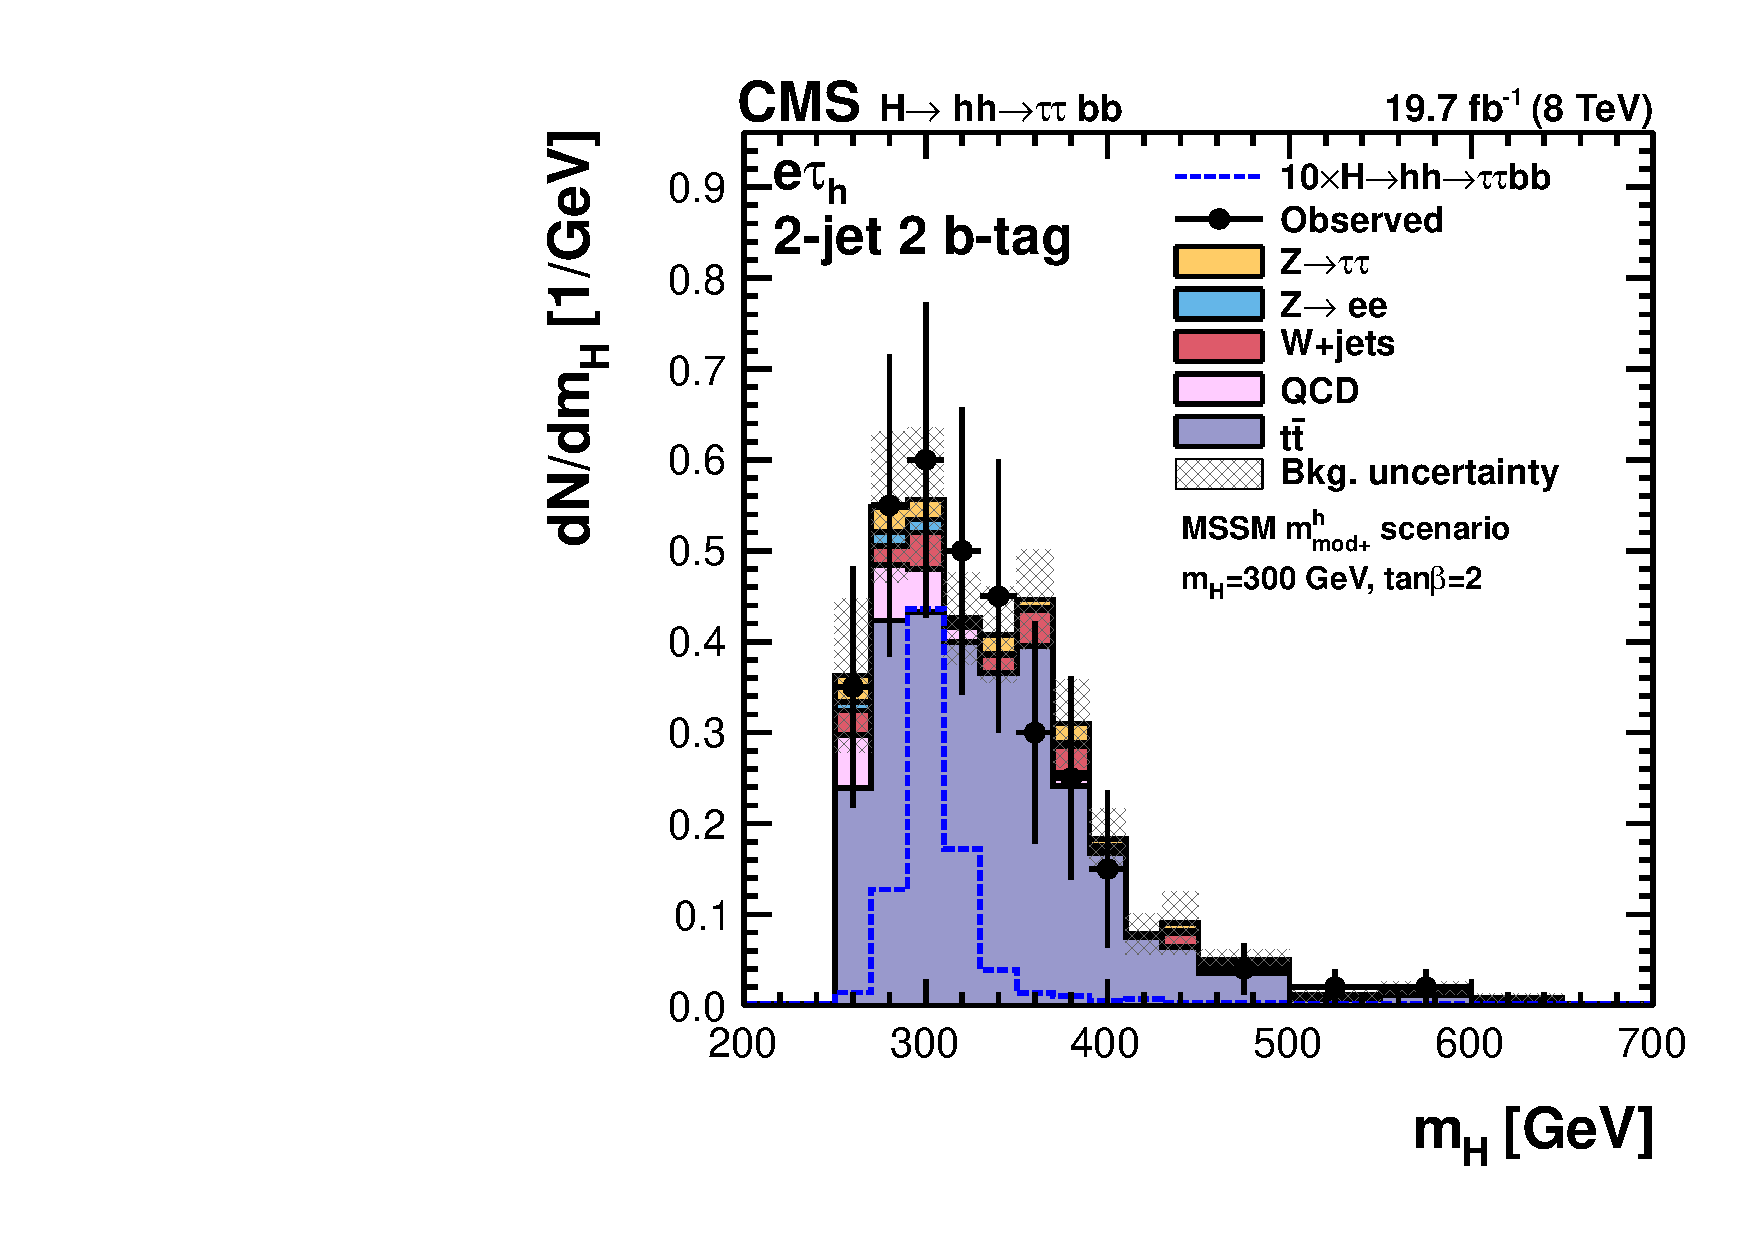
\includegraphics[width=0.5\textwidth]
      {plots/Hhh/eleTau_2jet2tag_postfit_8TeV_LIN.pdf}}
\end{center}
\caption{
Distributions of kinematic fit mass following the maximum likelihood fit for
events in the $\etau$ channel and the 2jet--0tag (top left) 2jet--1tag (top
right) and 2jet--2tag (bottom) categories. Signal is shown for a benchmark
cross-section times branching ratio for $m_{\PH}=300\,\GeV$ and $\tan\beta=2$
and scaled by a factor of 10 to make it visible.}
\label{fig:PostFitMHetau}
\end{figure} 

\subsection{Contribution from an SM Higgs boson}

\ac{SM} Higgs boson events are possible via both the $\PH\to\Pgt\Pgt$
and $\PH\to\Pqb\Pqb$ processes, and their contributions in these event
categories have been evaluated. The largest contribution occurs in the
2jet--0tag category, where gluon fusion production dominates. In the more signal
sensitive categories associated production, especially
$\PZ\PH\to\Pgt\Pgt\Pqb\Pqb$ or $\Pqb\Pqb\Pgt\Pgt$, is possible. 
However, these contributions are
reduced somewhat by the mass cuts on $m_{\Pqb\Pqb}$ and $m_{\Pgt\Pgt}$, and 
are less than $10\%$ when compared with the cross-section times branching ratio
the analysis is sensitive to in $\PH\to\Ph\Ph$. The effect on the expected limit
has been estimated by injecting the \ac{SM} signal and found to be smaller than
$3\%$. Thus it is sufficient to neglect the \ac{SM} contribution for now. In
future this relative contribution will become more important, as more data are
obtained and the analysis becomes more sensitive, and measures following those
described for the \ac{MSSM} $\Pphi\to\Pgt\Pgt$ analysis will need to be
employed. 

\subsection{Model Independent Results}

An expected limit on cross-section times branching ratio for the $\Hhh$
process is obtained using the methods described in \ref{sec:signalextraction}
with a signal strength modifier $\mu$ corresponding to the cross-section times
branching ratio in $\picobarn$. This result is analogous to the model independent
limits in the \ac{MSSM} analysis, except without the need to profile other
signal contributions. Figure \ref{fig:Hhhlimits} shows these
expected and observed limits for the $\etau$ and $\mutau$ channels separately.


\begin{figure}
\begin{center}
\subfloat[]{
    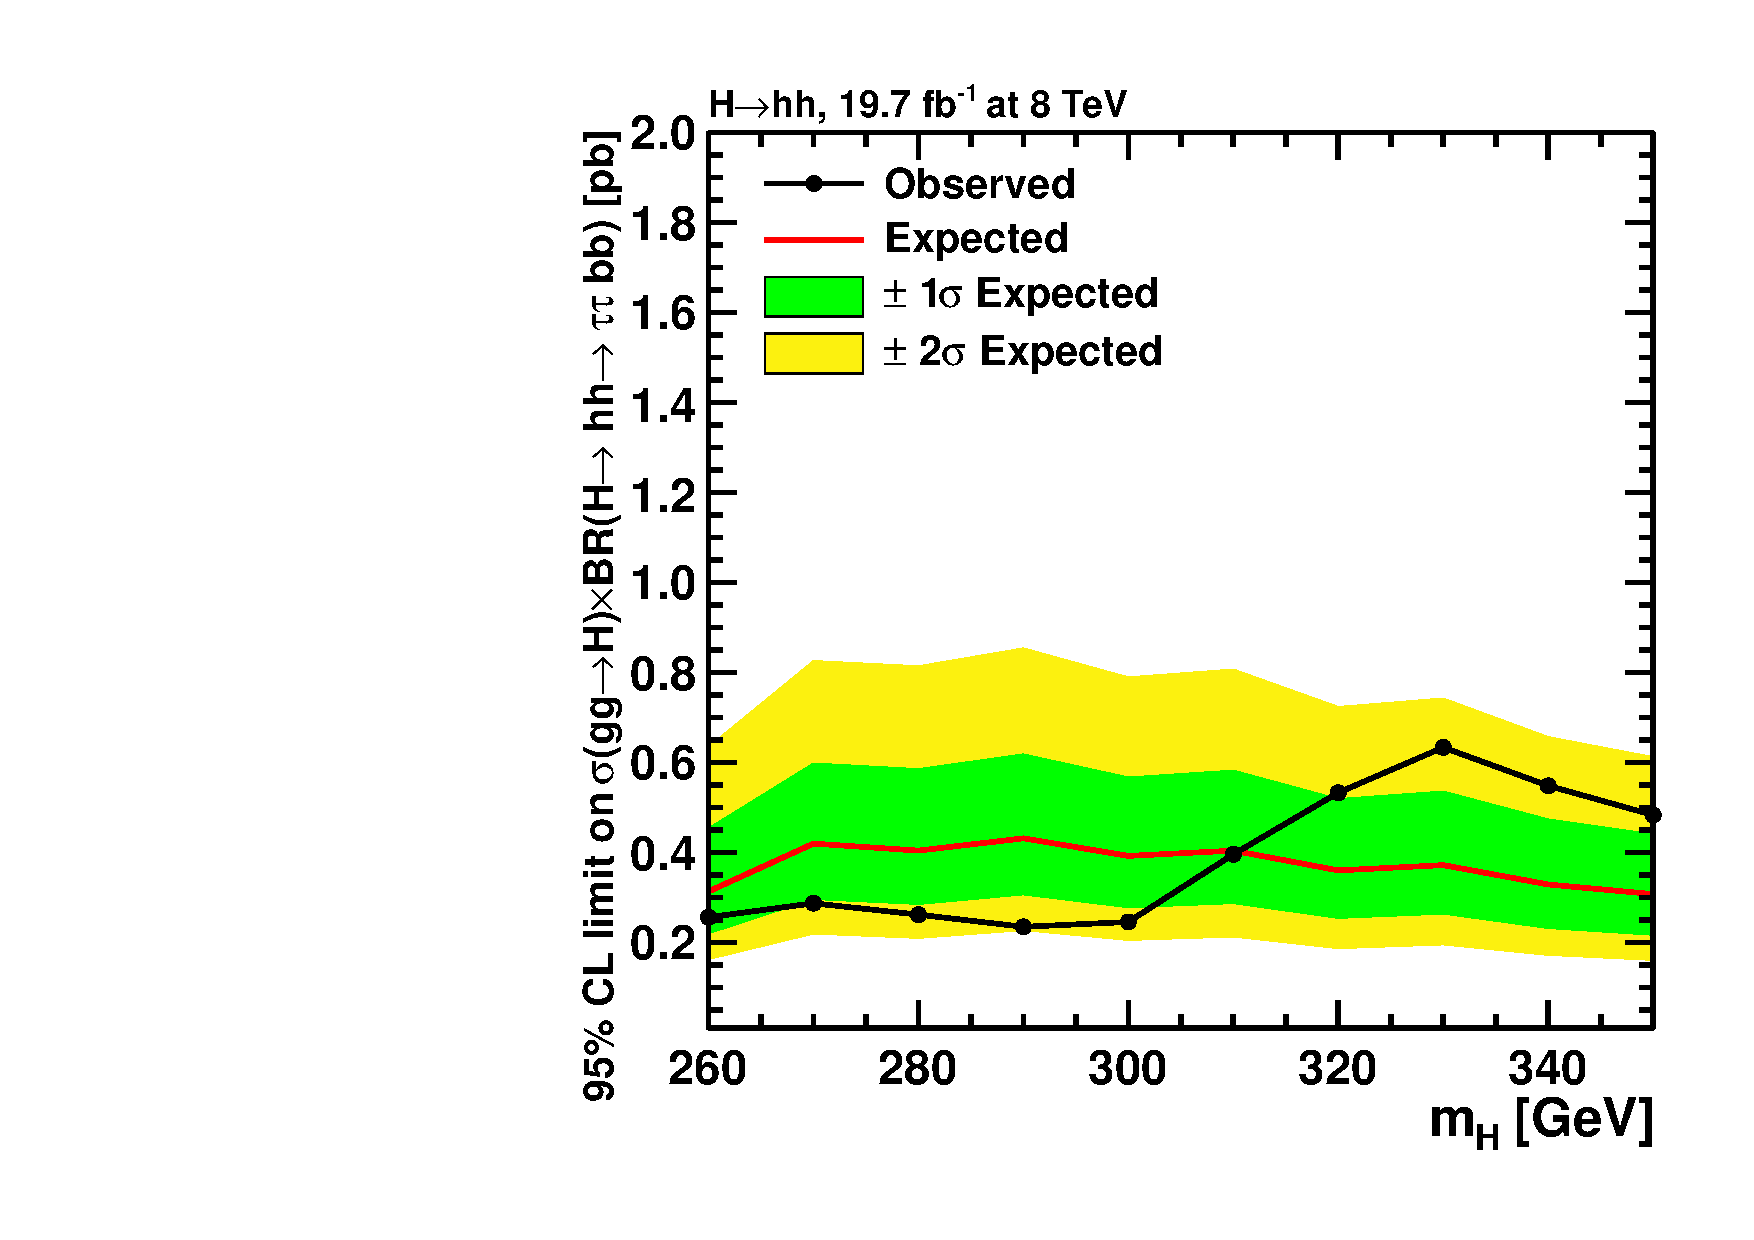
\includegraphics[width=0.5\textwidth]
      {plots/Hhh/mt_ggHTohh-limit.pdf}}
\subfloat[]{
    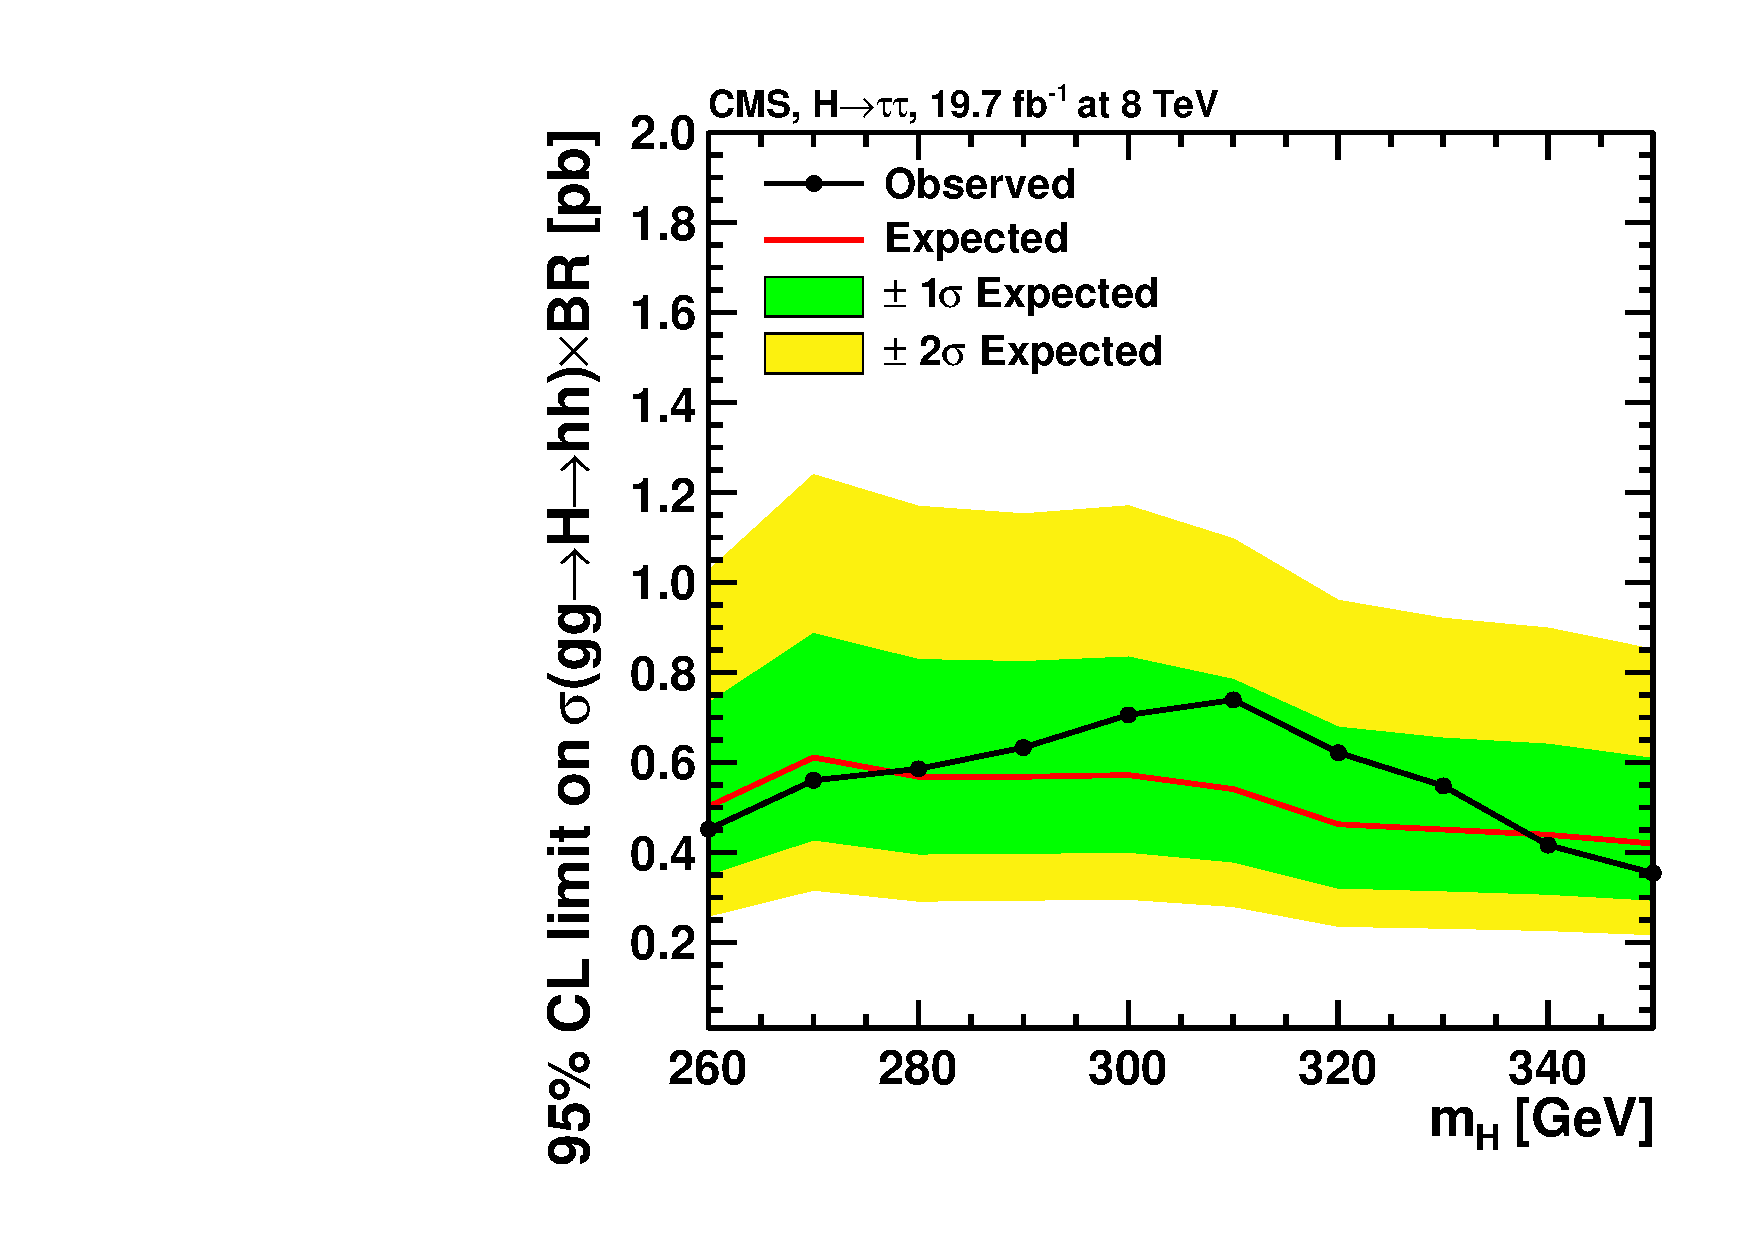
\includegraphics[width=0.5\textwidth]
      {plots/Hhh/et_ggHTohh-limit.pdf}}

\end{center}
\caption{
Expected and observed limits on cross-section times branching ratio for the
$\Pgluon\Pgluon\to\PH\to\Pgt\Pgt\Pqb\Pqb$ process for the $\mutau$ (left) and
$\etau$ (right) channels.}
\label{fig:Hhhlimits}
\end{figure} 

Figure~\ref{fig:HhhCmblimits} shows the result for the combination of the
$\etau$ and $\mutau$ channels (left) and a further combination with the fully
hadronic channel not described in this thesis (right).

\begin{figure}
\begin{center}
\subfloat[]{
    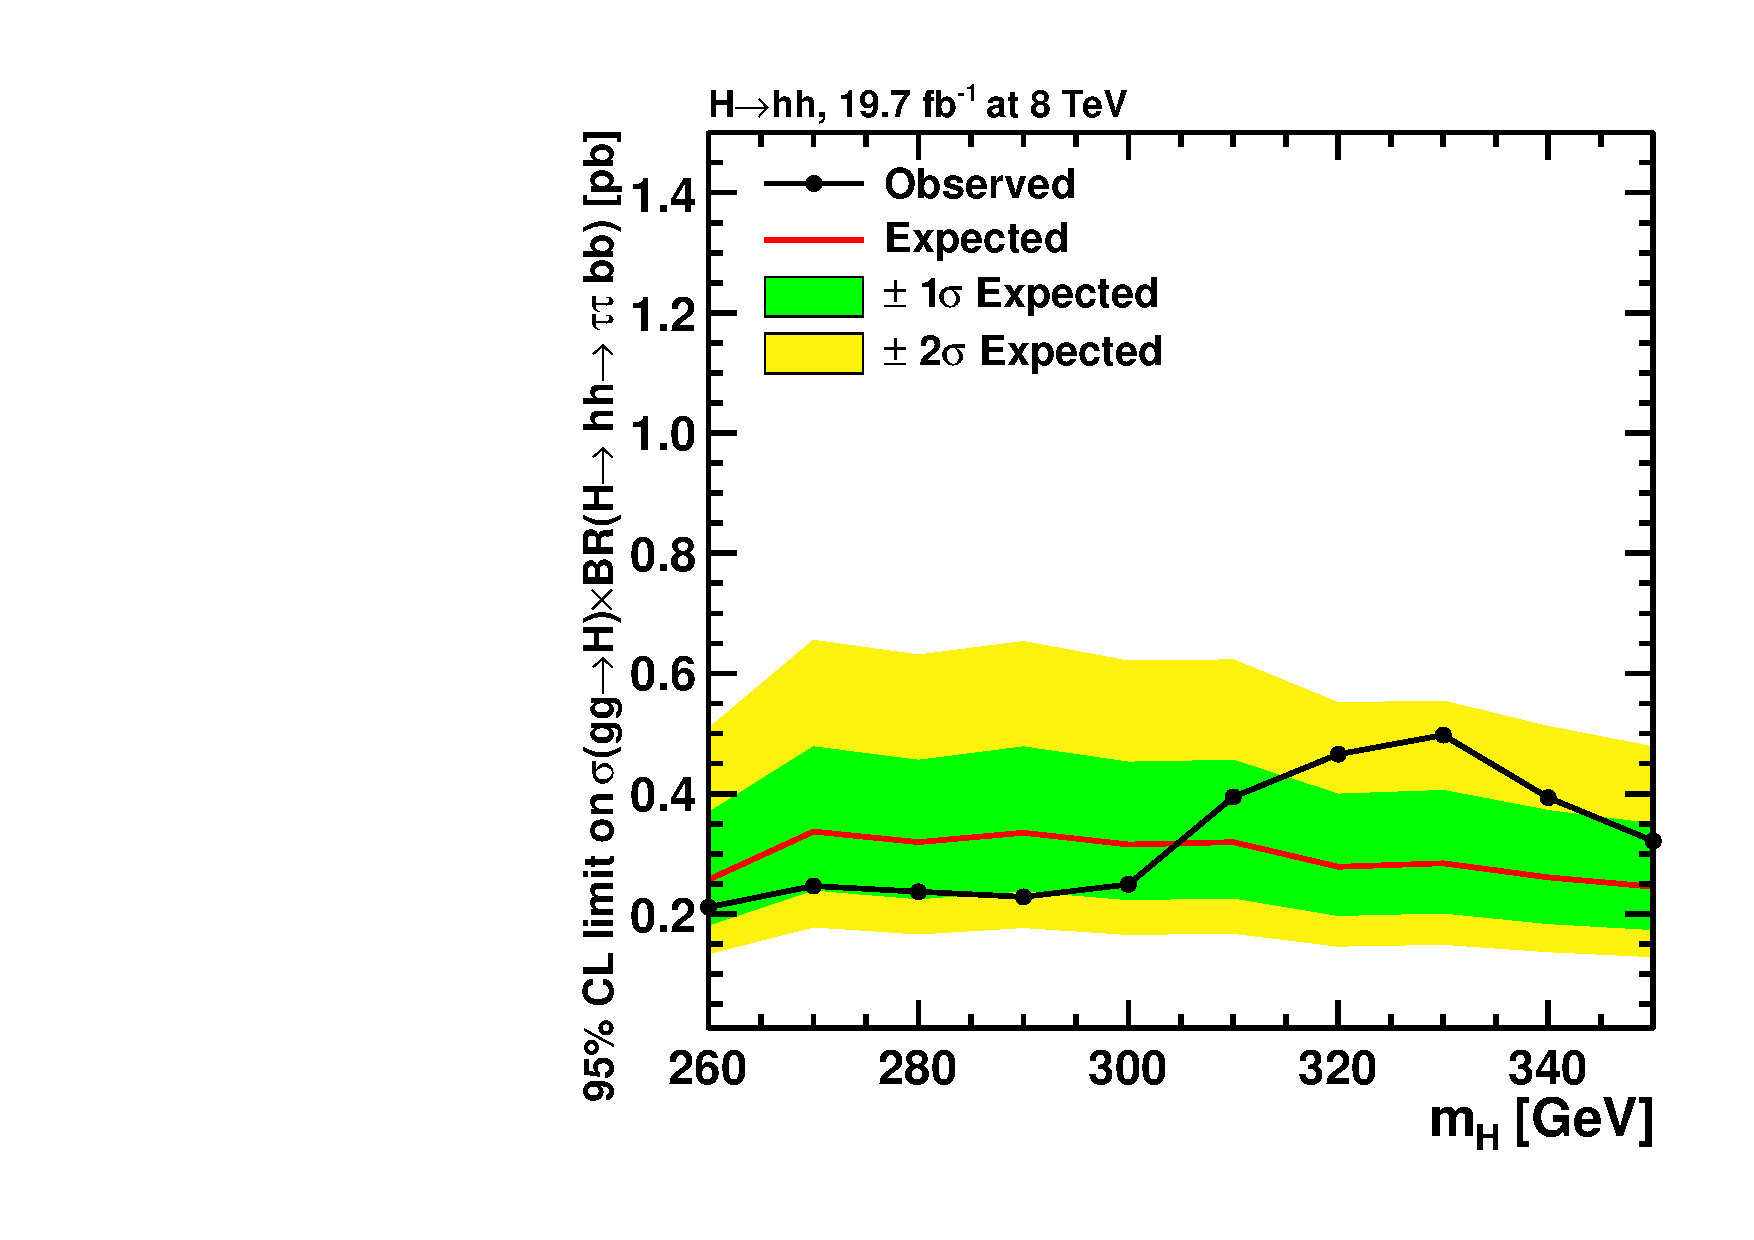
\includegraphics[width=0.5\textwidth]
      {plots/Hhh/et-mt_ggHTohh-limit.pdf}}
\subfloat[]{
    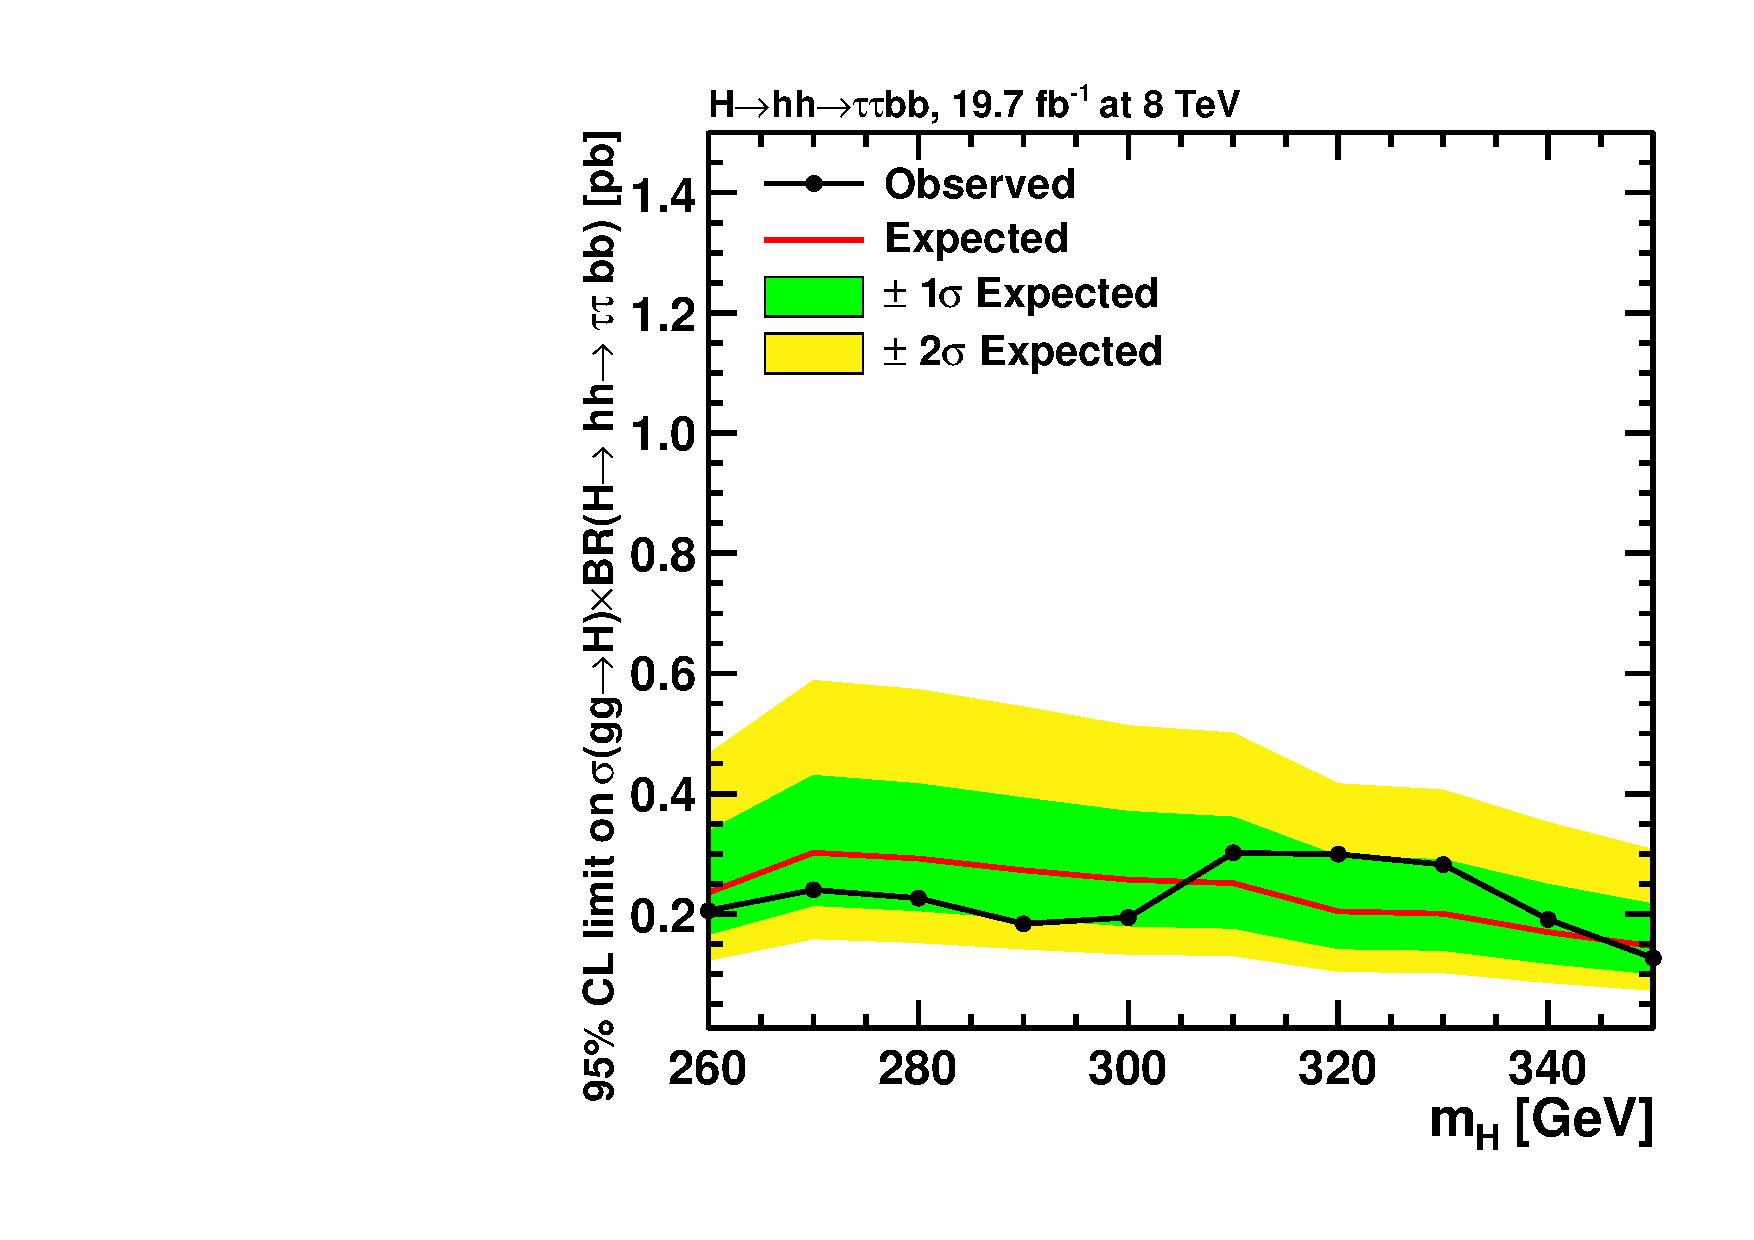
\includegraphics[width=0.5\textwidth]
      {plots/Hhh/cmb_ggHTohh-limit.pdf}}

\end{center}
\caption[Combined expected and observed limits on cross-section times branching ratio for the
$\Pgluon\Pgluon\to\PH\to\Pgt\Pgt\Pqb\Pqb$ process.]{
Combined expected and observed limits on cross-section times branching ratio for the
$\Pgluon\Pgluon\to\PH\to\Pgt\Pgt\Pqb\Pqb$ process. The left hand plot is the
combination of the $\etau$ and $\mutau$ channels discussed in this chapter, and
the right hand plot includes a combination with the $\tautau$ channel not
described in this thesis.}
\label{fig:HhhCmblimits}
\end{figure}

\subsection{Model Dependent Results}

As described in section~\ref{sec:lowtanbscenario}, this analysis is sensitive in
a particular region of \ac{MSSM} phase space at low $\tan\beta$, provided
appropriate choices are made for the radiative corrections which define the
benchmark scenario. Thus a model dependent result can be produced in such a
scenario, analogous to those described in~\ref{sec:modeldependent}. As discussed
above, this analysis is not so sensitive to the \ac{SM} Higgs boson boson, and hence
the special statistical treatment to separate the \ac{MSSM} and \ac{SM}
hypotheses is not required. Thus the limit in $m_{\PA}$--$\tan\beta$ is derived
by calculating the CL$_{s}$ values using the asymptotic approximation, comparing
the \ac{MSSM} signal hypothesis with the background-only hypothesis. The
resulting limit in the low-$\tan\beta$-high scenario for the combination of the
$\etau$ and $\mutau$ channels with the $\tautau$ channel is shown in
figure~\ref{fig:lowtanbhigh}. The lack of an excess of events in this analysis
allows a small amount of the low $\tan\beta$ phase space to be excluded.

\begin{figure}
\begin{center}
\subfloat[]{
    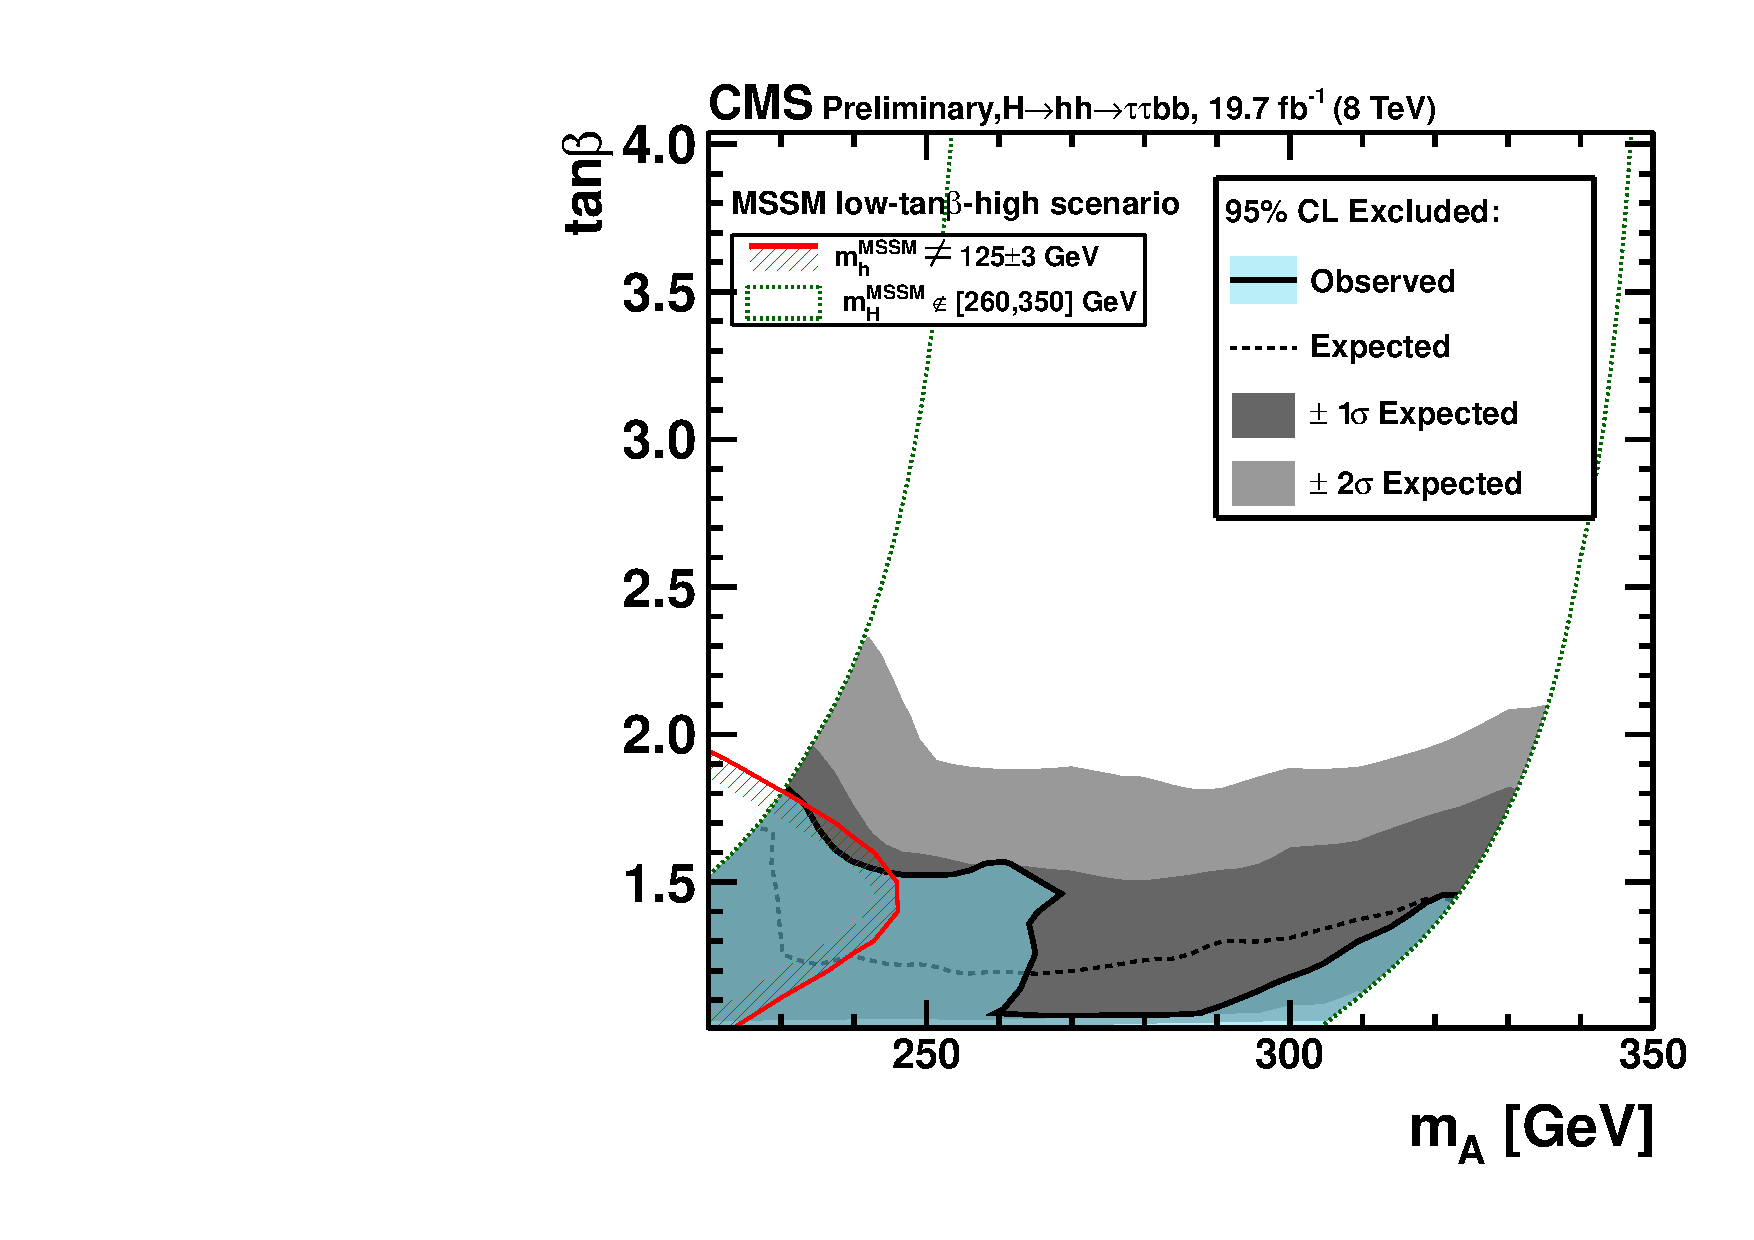
\includegraphics[width=0.7\textwidth]
      {plots/Hhh/cmb_low-tb-high-mA-tanb-hhh.pdf}}

\end{center}
\caption[Combined expected and observed limits in the $m_{\PA}-\tan\beta$ plane
of the low-$\tan\beta$-high scenario.]{
Combined expected and observed limits in the $m_{\PA}-\tan\beta$ plane
of the low-$\tan\beta$-high scenario.
This includes a combination with the $\tautau$ channel not
described in this thesis. The red area indicates the region of phase space which is already
excluded by the Higgs boson mass constraint of $125\pm3\,\GeV$. The grey area
indicates the region which is outside of the range of the $m_{\PH}$ values
considered in this analysis. The lack of an excess of events in this analysis
allows a small amount of the low $\tan\beta$ phase space to be excluded.}
\label{fig:lowtanbhigh}
\end{figure}
